\documentclass[a4paper,12pt,twoside,onecolumn,openright,svgnames]{book}

%%%%%%%%%%%%%%%%%%%%%%%%%% PAQUETES IMPORTANTES
\usepackage[a4paper,left=2cm,top=2.5cm,right=1.5cm,bottom=2.5cm]{geometry}
\usepackage[utf8]{inputenc}       % códificación de símbolos
\usepackage{amsmath}
\usepackage{amssymb}          % \checkmark y otros símbolos matemáticos
\usepackage[spanish,es-tabla,es-nodecimaldot]{babel}
\unaccentedoperators              % babel acentúa operadores math. por defecto
\usepackage{times}                % (times roman, helvetica, courier)
\usepackage[official]{eurosym}    % €€€
\usepackage{graphicx}             % Imprescindible para gráficos
\usepackage{svg}                  % para incluír gráficos svg
% \usepackage{svg-inkscape}       % útil con inkscape
\usepackage{xurl}                  % para que latex pueda partir URLs
\usepackage{ltxtable}             % para usar \LTXtable
\usepackage{xcolor}     % Texto en color diferente
\usepackage{booktabs}

%%%%%%%%%%%%%%%%%% ANTES DE AÑADIR UN PAQUETE COMPRUEBA SI ESTÁ EN ESTA
%%%%%%%%%%%%%%%%%% LISTA Y BUSCA LA DOCUMENTACIÓN PUES SI AÑADES UNO
%%%%%%%%%%%%%%%%%% PUEDE COLISIONAR CON UNO DE ESTOS.
%%%%%%%%%%%%   PACKAGES PARA CODIGO Y LISTADOS
% minted para listados:
%     https://www.overleaf.com/learn/latex/Code_Highlighting_with_minted
\usepackage[newfloat]{minted}
\usepackage{listings} % es compatible con minted (para otros listados)
\renewcommand{\lstlistingname}{Código}
\renewcommand{\lstlistlistingname}{Índice de \lstlistingname s}
\newenvironment{code}{\captionsetup{type=listing}}{}
\SetupFloatingEnvironment{listing}{name=Código Fuente}

%%%%%%%%%%%%%  UTILIDADES
\usepackage{pdfpages}   % Incluir pdfs como paginas del documento (para anexos)
\usepackage[hidelinks]{hyperref} % para incluir links intra/extra documento
\usepackage{colortbl}   % tablas con colores
%%% Tablas, arrays, etc.
\usepackage{tabularx}   % Nuevo tipo de columna en tabla X, se ajusta al tamaño
\usepackage{multirow}   % Para tablas con multifilas
\usepackage{array}      % Para los nuevos tipos de columnas en tabla

%%%%%%%%%%%%%  PACKAGES QUE DAN CONTROL EXTRA A VARIAS ORDENES
% caption para gestionar los listados en floats -como figuras o tablas-
\usepackage{caption}              % con mejor control de captions
\usepackage{setspace}             % facilita la gestión de distancias
\usepackage{cite}                 % mejora aspecto bibliografía numérica
\usepackage[toc,page]{appendix}   % control extra para apéndices.
\usepackage{subfig}               % para figuras dentro de figuras
\usepackage{float}                % mejor control de posiciones en float
\usepackage{xspace}               % busca pequeños errores en nombres latex
\usepackage{enumitem}             % http://ctan.org/pkg/enumitem
\usepackage[nottoc,notlot,notlof]{tocbibind} % bibliografía a tabla Contenidos

%%%%%%%%%%%%% TUNEO DE DISTANCIAS Y PEQUEÑOS DETALLES
\renewcommand{\arraystretch}{1.5} % padding tablas
\renewcommand{\baselinestretch}{1.2} % (latex neutro) esponja el texto.
\setlength{\parindent}{0.5cm}     % sangrado de primera línea de párrafo.
\usepackage{microtype}            % Soluciona algunos problemas de Overfullness
\usepackage[section]{placeins}    % Fuerza a que los floats se queden en su section
\addtolength{\parskip}{1em}       % Separa un poquito los parrafos

%%%%%%%%%%%%%%%  FIN DE PAQUETES (no deberías incluír ninguno fuera de aquí)

\begin{document}
   \raggedbottom
   \addtolength{\headsep}{4mm}
   % Material inicial del documento.
   % Esta sección va en número romanos en minúscula.
   \frontmatter
      % He organizado los archivos como me gusta. Siéntete libre
      % de crear las carpetas que creas necesario.
      \begin{titlepage}
\centering
% Logo de la universidad

\includegraphics[width=0.4\textwidth]{images/uva_logo.pdf}
\vspace{1cm}

% Escuela
{\fontfamily{prm}\LARGE Escuela de Ingeniería Informática de Segovia\par}
\vspace{1cm}

% Tipo de trabajo
{\large \textbf{\scshape Trabajo de Fin de Grado}\par}
\vspace{0.6cm}

% Grado
{\large\sffamily Grado en Ingeniería Informática\\
de Servicios y Aplicaciones\par}
\vspace{1.2cm}

% Título del trabajo (ajustable en varias líneas si es largo)
{\Large\sffamily\bfseries
\begin{minipage}{0.9\textwidth}
\centering
Uso de GraphRAG con Inferencia Local para el Análisis Inteligente de Pliegos Técnicos
\end{minipage}
\par}
\vspace{2cm}

\vfill

% Datos del autor y tutor
\begin{flushright}
    {\normalsize\textbf{Autor:}}\\
    {\large Daniel Gómez Arranz\par}
    \vspace{0.3cm}

    {\normalsize\textbf{Tutor:}}\\
    {\large Dr. José Vicente Álvarez Bravo\par}
    \vspace{0.3cm}

    {\normalsize\textbf{Fecha:}}\\
    {\large Mayo 2026}
\end{flushright}

\end{titlepage}

      \chapter*{Agradecimientos}
\addcontentsline{toc}{chapter}{Agradecimientos}

En primer lugar, quiero expresar mi más sincero agradecimiento a mi tutor, el Dr. José Vicente Álvarez Bravo, por su orientación, dedicación y apoyo a lo largo de todo el desarrollo de este trabajo, que, aun con todos los retrasos del mismo por varios motivos, nunca dejó de prestar su apoyo. Sus comentarios y sugerencias han sido fundamentales para dar forma a este proyecto.

Gracias también a la Escuela de Ingeniería Informática de Segovia y a la Universidad de Valladolid por la formación recibida durante estos años, y por poner a disposición de los alumnos los recursos necesarios para llevar a cabo proyectos de este tipo.

Por último, mi agradecimiento más profundo a mi familia , pareja y amigos, cuyo apoyo incondicional ha sido un pilar esencial durante el viaje que ha resultado ser la carrera.

      

\ 

\vskip 2cm

{\noindent\bfseries\Huge Resumen}

\vskip 1cm

Los Modelos de Lenguaje (LLM) representan una de las ramas de la inteligencia artificial que más avances ha experimentado en los últimos años. Uno de los principales desafíos que presentan, tanto por su coste computacional como por las limitaciones que afectan directamente al usuario, es la cantidad de tokens que pueden procesar. En este trabajo se estudian en profundidad los LLMs, su funcionamiento, el uso de agentes, y se plantean soluciones prácticas al problema del contexto.
\\
\vskip 1cm

Como parte del desarrollo, se ha implementado una solución personalizada para un caso empresarial concreto, cuyo enfoque puede extrapolarse a otros ámbitos. Para ello, se ha desplegado en local un servidor de Ollama con distintos modelos de lenguaje, al que se le han alimentado documentos extensos (de más de 100 páginas). A partir de estos, el sistema permite realizar preguntas al modelo sobre el contenido.
\\
\vskip 1cm

Para lograrlo, se han utilizado técnicas de segmentación del contenido en chunks, así como agentes, rerankers, y un sistema de búsqueda con bases de datos vectoriales basadas en grafos mediante LangGraph, realizando una modificación del conocido Retrieval Augmented Generation(RAG) , el cual explicaremos con más detalle posteriormente. La combinación de estas tecnologías, aplicadas desde Python, ha permitido construir un chatbot capaz de responder preguntas de forma eficiente, utilizando únicamente modelos que pueden ejecutarse en local.

\vskip 1cm

Finalmente, haremos un pequeño estudio de la importancia de la calidad del propio modelo usado, comparando los resultados de algunos de los modelos locales, con los proporcionados con la API de ChatGPT (Haciendo primero nuestro tratamiento de los datos).

\textbf{Palabras clave:} LLM, Python, Agentes, LangChain, LangGraph, Ollama, Retrieval-Augmented Generation (RAG), modelos locales, búsqueda semántica, bases de datos vectoriales.

\newpage
\newpage

{\bfseries\Huge Abstract}

\vskip 1cm
Large Language Models (LLMs) have become one of the most rapidly evolving branches of Artificial Intelligence in recent years. However, one of the main challenges they face is their limited token window, which directly impacts computational cost and user experience. This project explores in depth the functioning of LLMs, the use of agents, and proposes practical solutions to the context length limitation.
\vskip 1cm
A custom solution was implemented to address a specific business problem, with the aim of building a scalable and locally hosted chatbot. Using Ollama to run various local LLMs, the system is able to answer user questions about large sets of documents (exceeding 100 pages). To achieve this, we applied content chunking techniques, as well as tools such as agents, rerankers, and a semantic search system based on graph-structured vector databases using LangGraph. This setup represents a customized version of Retrieval-Augmented Generation (RAG).
\vskip 1cm
All components were integrated using Python, and the solution enables efficient document querying using only locally executed models. Finally, we provide a brief comparison between the performance of local models and ChatGPT API-based results, after applying our own preprocessing pipeline.
\vskip 1cm
\textbf{KeyWords:} LLM, Python, LangChain, LangGraph, Retrieval-Augmented Generation, local models, semantic search, Ollama, agents.
      \tableofcontents
      \listoffigures
      \listoftables
   % Material principal del documento
   % Esta sección va en números arábicos desde el 1
   % Los títulos y tipos de capítulos sólo son para muestra
   % y tu memoria puede tener otros distintos.
   \mainmatter
      \chapter{Introducción}\label{cap1}

\section{Introducción}
\textbf{La Inteligencia Artificial (IA)} ha ido integrándose de forma progresiva en múltiples aspectos de la vida cotidiana. Aunque sus orígenes se puedan trazar a hace varias décadas, no ha sido hasta los últimos años cuando el público general ha empezado a interactuar de forma consciente con sistemas inteligentes. Algunos ejemplos son los vehículos autónomos como los de Tesla, o los sistemas de clasificación automática de fotografías en dispositivos móviles.

Sin embargo, el mayor punto de inflexión en la percepción social de la IA ha sido la aparición de los \textit{Large Language Models} (LLM), cuyo impacto ha sido especialmente notorio a través de interfaces conversacionales como ChatGPT. Para ilustrar su crecimiento, se muestra a continuación la evolución del número de consultas diarias a este tipo de sistemas:

\vskip 0.15cm
\begin{figure}[H]
    \centering
    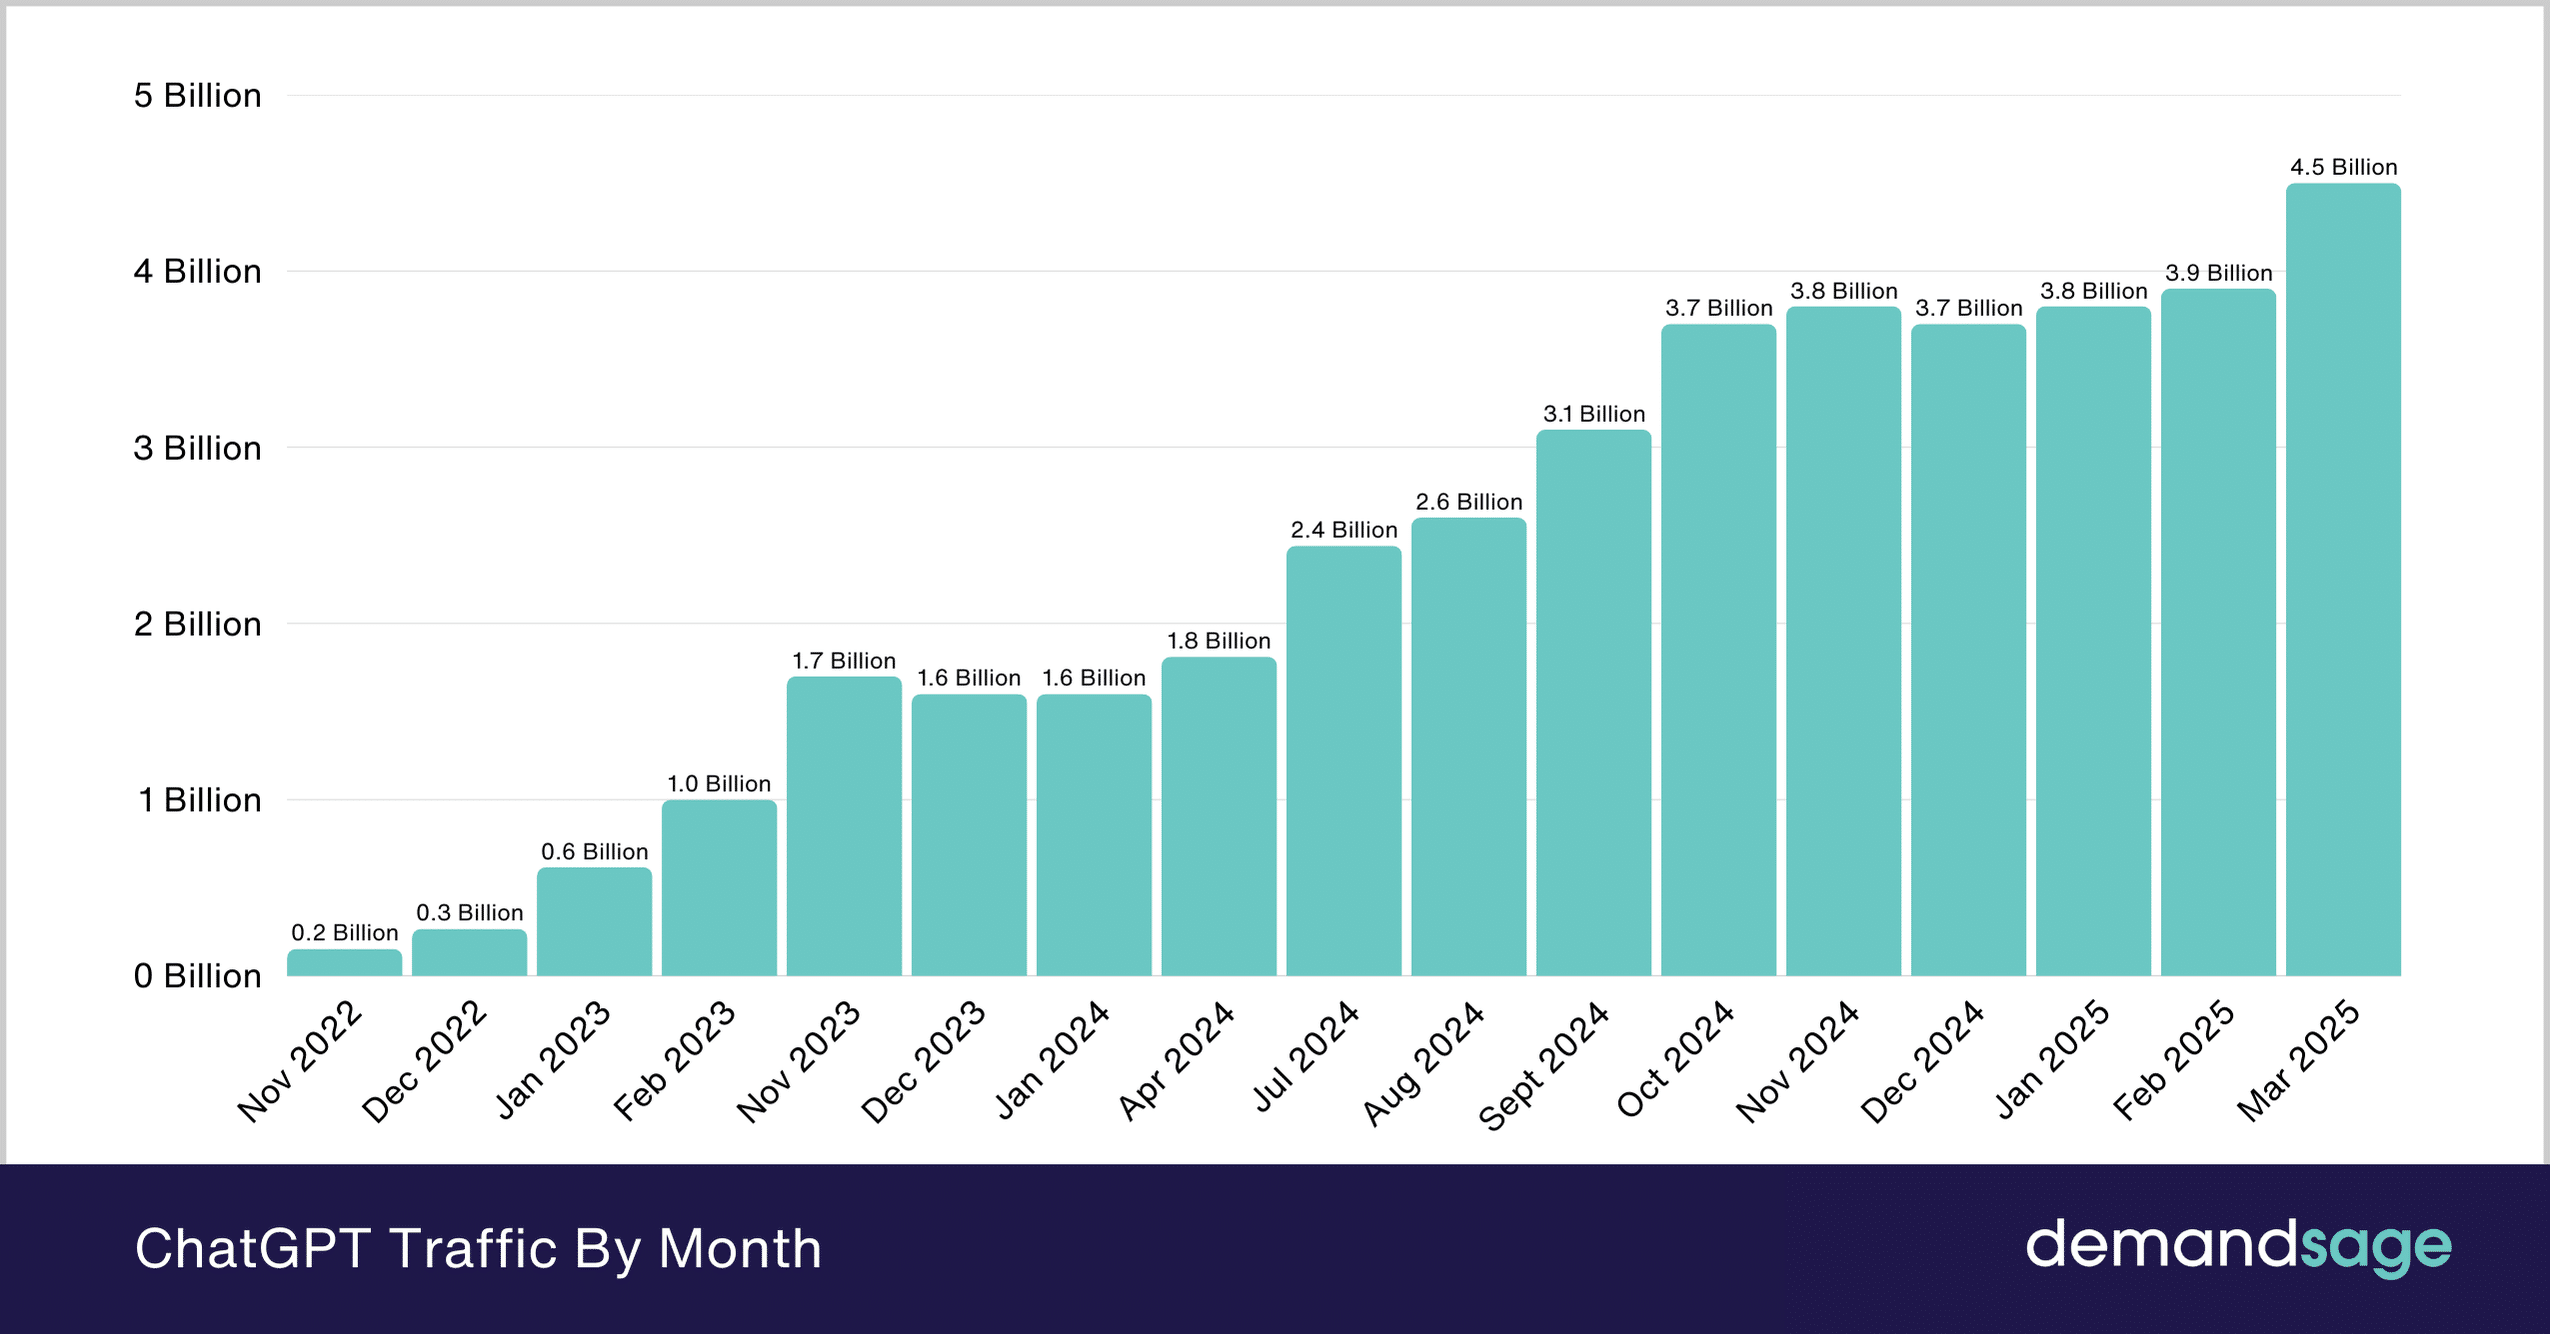
\includegraphics[width=0.75\textwidth]{images/ChatGPTTraffic.png}
    \caption{Evolución del número de consultas diarias (en miles de millones) a ChatGPT \cite{ChatGPTTraffic}.}
    \label{data_evolution}
\end{figure}

Como se observa, la tendencia es claramente ascendente, y la adopción de este tipo de modelos continúa expandiéndose en múltiples sectores. En particular, su uso en el ámbito académico y empresarial se ha vuelto cada vez más común, no solo para generar respuestas simples, sino para realizar tareas complejas como la comprensión y el análisis de documentos extensos.

\vspace{0.3cm}
\textbf{Propósito y objetivos de este trabajo}

Este Trabajo de Fin de Grado aborda un problema concreto: la \textbf{consulta local y privada de documentos técnicos extensos} —en particular, pliegos de contratación pública de entre 30 y 100 páginas— mediante la arquitectura \textit{GraphRAG} (\textit{Retrieval-Augmented Generation} con grafos de conocimiento). El sistema permite formular preguntas en lenguaje natural sobre dichos documentos sin enviar información a servicios externos, combinando recuperación semántica, un grafo de conocimiento jerárquico y agentes de decisión. Sus objetivos principales son:

\begin{itemize}
    \item Desarrollar un módulo de segmentación jerárquica de documentos PDF que preserve la estructura de secciones y subsecciones tal como aparece en el índice original.
    \item Construir un grafo de conocimiento documental que codifique relaciones jerárquicas, secuenciales y semánticas entre los fragmentos de texto.
    \item Implementar agentes de decisión que seleccionen dinámicamente la estrategia de recuperación más adecuada para cada consulta del usuario.
    \item Validar el sistema sobre documentos reales, cuantificando la mejora frente al RAG vectorial tradicional mediante métricas automáticas y un estudio de ablación por componentes.
    \item Demostrar la viabilidad de un despliegue completamente local, sin envío de datos a servidores externos, adecuado para entornos con requisitos de privacidad estrictos.
\end{itemize}

\textbf{Alcance del trabajo.} El sistema se diseña y valida sobre pliegos de prescripciones técnicas y cláusulas administrativas en español, dominio en el que se concentran tanto el diseño del extractor jerárquico como la mayor parte de la evaluación experimental. Se incluye una prueba de generalización sobre documentos de ciberseguridad (véase Capítulo~\ref{cap7}), pero la extensión sistemática a otros dominios documentales queda fuera del alcance de este TFG. Los resultados de la evaluación deben interpretarse como evidencia exploratoria: los tamaños de muestra empleados —entre 8 y 50 preguntas según el experimento— son adecuados para un trabajo de esta naturaleza, pero no permiten establecer conclusiones estadísticamente robustas ni generalizar el rendimiento a cualquier tipo de documento o consulta.

La motivación concreta que originó este trabajo —tanto personal como empresarial— se desarrolla en el Capítulo~\ref{cap3}. Las secciones siguientes establecen el marco teórico necesario para comprender los fundamentos tecnológicos sobre los que se construye la solución.
\newpage
\section{Marco Teórico.}

\subsection{Definición del Problema Central}\label{sec:problema_central}

El problema central que aborda este trabajo puede formularse del siguiente modo: dado un conjunto de documentos técnicos extensos —en concreto, pliegos de prescripciones técnicas y cláusulas administrativas de contratación pública, con un tamaño habitual de entre 30 y 100 páginas—, el objetivo es construir un sistema que permita a un usuario formular preguntas en lenguaje natural y obtener respuestas fundamentadas en el contenido del propio documento, de forma completamente local, sin enviar información a servicios externos.

Este problema presenta tres retos técnicos fundamentales que justifican la arquitectura propuesta:

\begin{enumerate}
    \item \textbf{Limitación de la ventana de contexto:} Los modelos de lenguaje desplegables localmente en hardware de usuario (modelos de 7B--13B parámetros) operan con ventanas de contexto de 8.000--32.000 tokens, muy por debajo de los 60.000 o más tokens que puede contener un documento técnico completo. Enviar el documento íntegro al modelo no es posible en la mayoría de casos.
    \item \textbf{Pérdida de jerarquía documental:} Los sistemas RAG tradicionales dividen el documento en fragmentos independientes, perdiendo las relaciones padre-hijo entre secciones. Una subsección breve (p.ej. ``1.2.3. Requisitos de anclaje'') carece de significado sin el contexto de su sección padre (``1.2. Rack de comunicaciones'').
    \item \textbf{Privacidad y soberanía del dato:} Los pliegos de contratación pública pueden contener información estratégica y comercial sensible que no puede ser procesada en plataformas de nube de terceros sin riesgo legal o de cumplimiento normativo.
\end{enumerate}

La solución propuesta —el sistema \textit{GraphRAG} local— combina la recuperación semántica con un grafo de conocimiento jerárquico y agentes de decisión, abordando simultáneamente los tres retos enumerados. Las secciones siguientes del marco teórico proporcionan los fundamentos conceptuales de cada componente de esta solución: los modelos de lenguaje y sus limitaciones, la arquitectura RAG, los agentes inteligentes y las bases de datos vectoriales.

\subsection{Inteligencia Artificial: Conceptos Generales}
La Inteligencia Artificial puede definirse como el campo de estudio que busca dotar a las máquinas de capacidades cognitivas similares a las del ser humano.
La IA es un campo muy extenso que reúne un conjunto de conceptos que le permiten imitar capacidades intrínsecamente humanas, como el aprendizaje, el reconocimiento de formas, la percepción o la resolución de problemas complejos.
Para llevar a cabo estas tareas se nutre de una amplia variedad de disciplinas, como las matemáticas, la lógica, la informática, e incluso otras como la neurociencia o la lingüística.

\vspace{0.3cm}
\textbf{Clasificación de la IA}

La IA puede clasificarse de distintas formas, siendo las más comunes:

\begin{itemize}
    \item \textbf{Por nivel de capacidad:}
    \begin{itemize}
        \item \textbf{IA débil o estrecha:} Diseñada para realizar tareas específicas (ej. clasificación de imágenes, asistentes por voz(Amazon Alexa)), incluso algunos LLMs como ChatGPT o DeepSeek entran en este nivel, hoy en día es el único tipo de IA que existe.
        \item \textbf{IA general o sólida:} Capaz de realizar cualquier tarea cognitiva humana, esta IA, es capaz de utilizar conocimientos y habilidades previamente aprendidas para la resolución de las mismas, a día de hoy, es simplemente un concepto teórico.
        \item \textbf{Súper IA:} Al igual que la IA general, es meramente una suposición teórica. De hacerse realidad, pensaría, aprendería y razonaría de manera superior a la humana; estas aplicaciones teóricas habrían evolucionado hasta el punto de comprender aspectos humanos como los sentimientos.
    \end{itemize}

    \item \textbf{Por funcionalidades:}
    \begin{itemize}
        \item \textbf{IA mecánica reactiva:} Sistemas que siguen instrucciones explícitas para realizar una tarea específica, sin capacidad de recordar resultados o decisiones anteriores, trabajando únicamente con los datos disponibles en el momento. Esta rama proviene de la matemática estadística y es capaz de analizar grandes cantidades de datos (por ejemplo, el motor de recomendaciones de Netflix usa el historial de visualización para recomendar contenido con mayor probabilidad de ser del agrado del usuario).
        \item \textbf{IA de memoria limitada:} Sistemas que pueden recordar eventos y resultados pasados, permitiendo utilizar estos datos para decidir el curso de acción más probable con el fin de lograr el resultado esperado.
        Estos datos, no se retienen de manera tradicional guardándolos en algún lugar, sino que es entrenada con esos datos, permitiendo mejorar el rendimiento con un mayor número de datos.
        Algunos ejemplos son la IA Generativa (ChatGPT...), vehículos autónomos...
        \item \textbf{IAs con funcionalidades teóricas:} Abarca tanto la teoría de la mente en IA como la IA autoconsciente; ambas son aún teóricas. La primera sería capaz de analizar datos (voces, imágenes, etc.) con el fin de comprender pensamientos y emociones y simular relaciones similares a las humanas, mientras que la IA autoconsciente sería capaz de comprender emociones y pensamientos humanos y desarrollar los propios.
    \end{itemize}
\end{itemize}

A continuación, se presenta una tabla resumen de los principales tipos de IA según distintos criterios de clasificación.

\vspace{0.5cm}
\begin{table}[H]
\centering
\caption{Clasificación de la Inteligencia Artificial}
\begin{tabular}{|p{3.5cm}|p{4.5cm}|p{6cm}|}
\hline
\textbf{Criterio} & \textbf{Tipo de IA} & \textbf{Descripción y ejemplos} \\
\hline
\multirow{3}{*}{\textbf{Por capacidad}} 
& IA débil & Especializada en tareas concretas. Ej: Alexa, Siri, ChatGPT. \\
& IA general & Teórica. Capaz de realizar cualquier tarea cognitiva humana. \\
& Súper IA & Hipotética. Superaría al ser humano en inteligencia y emociones. \\
\hline
\multirow{3}{*}{\textbf{Por funcionalidad}} 
& Mecánica reactiva & No guarda memoria. Reacciona en tiempo real. Ej: Recomendaciones de Netflix. \\
& Memoria limitada & Aprende de datos previos. Ej: ChatGPT, vehículos autónomos. \\
& IA teórica & Incluye teoría de la mente y autoconsciencia. Aún no desarrolladas. \\
\hline
\end{tabular}
\label{tab:clasificacion_ia}
\end{table}


\newpage
\textbf{Machine Learning (ML)}

El \textit{Machine Learning} es una rama de la IA que se centra en el entrenamiento de las máquinas con el fin de imitar el aprendizaje humano, siendo así capaces de realizar tareas de forma autónoma y de mejorar su rendimiento mediante una mayor exposición a datos y la propia experiencia con los mismos.
De acuerdo con \cite{ibmML2024}, un sistema de aprendizaje automático puede describirse a través de tres componentes fundamentales:

    \begin{itemize}
        \item \textbf{El proceso de decisión:} Generalmente los algoritmos de Machine Learning son utilizados para realizar predicciones o clasificaciones en base a unos datos de entrada (etiquetados o no) de los cuales el algoritmo hará una estimación.
        \item \textbf{Función de error:} Es aquella función que 
        compara los resultados con ejemplos conocidos para evaluar el desempeño del algoritmo.
        \item \textbf{Optimización del modelo:} Un método mediante el cual el algoritmo evalúa los fallos y actualiza el proceso de decisión (Principalmente mediante pesos), este procedimiento generalmente es repetido de manera iterativa.
    \end{itemize}

A continuación, sin entrar en profundidad en las implementaciones, se describen los principales tipos de aprendizaje automático:

\begin{itemize}
    \item \textbf{Aprendizaje supervisado:} Se utilizan datos etiquetados para el entrenamiento, con el fin de clasificar o predecir resultados; los pesos del modelo se ajustan a medida que se introducen datos. (Ejemplos: Regresión Lineal, Random Forest y Máquinas de Soporte Vectorial (SVM).)
    \item \textbf{Aprendizaje no supervisado:} Se emplean algoritmos de \textit{Machine Learning} para clasificar conjuntos de datos sin etiquetar, es decir, sin necesidad de intervención humana directa para las agrupaciones. (Ejemplos: Clustering, Reducción de Dimensionalidad y \textit{Autoencoders}.)
    \item \textbf{Aprendizaje semisupervisado:} Punto intermedio entre los dos tipos anteriores; combina un pequeño conjunto de datos etiquetados con uno mayor sin etiquetar, lo que permite paliar el problema de la escasez de datos etiquetados.
    \item \textbf{Aprendizaje por refuerzo:} En cierto modo similar al aprendizaje supervisado, pero en lugar de utilizar datos de muestra, el modelo aprende mediante prueba y error, reforzando la secuencia de acciones que produce resultados más exitosos.
\end{itemize}

\vspace{0.5cm}
\begin{table}[H]
\centering
\caption{Resumen Tipos de aprendizaje en Machine Learning}
\begin{tabular}{|p{3.5cm}|p{6cm}|p{4.5cm}|}
\hline
\textbf{Tipo de aprendizaje} & \textbf{Descripción} & \textbf{Ejemplos comunes} \\
\hline
\textbf{Supervisado} & Utiliza datos etiquetados. El algoritmo aprende una función a partir de pares entrada-salida. & Regresión lineal, Random Forest, SVM. \\
\hline
\textbf{No supervisado} & Usa datos sin etiquetar. El modelo identifica patrones o estructuras ocultas. & Clustering, PCA, Autoencoders. \\
\hline
\textbf{Semisupervisado} & Combina un pequeño conjunto etiquetado con una gran cantidad sin etiquetar. Reduce necesidad de anotaciones humanas. & Clasificadores combinados con técnicas de propagación de etiquetas. \\
\hline
\textbf{Por refuerzo} & Aprende mediante prueba y error. Recibe recompensas o penalizaciones según su rendimiento. & Robots autónomos, sistemas de control de videojuegos. \\
\hline
\end{tabular}
\label{tab:tipos_aprendizaje}
\end{table}


\newpage
\textbf{Diferencias entre Deep Learning (DL), Machine Learning (ML) y Neural Networks (NN)}

Con frecuencia, estos términos se utilizan de manera indistinta; a continuación se presenta una diferenciación precisa de cada uno antes de profundizar en los LLMs.

El \textbf{Deep Learning (DL)} es un subcampo dentro de las \textbf{Redes Neuronales Artificiales (NN)}, las cuales, a su vez, son un subcampo del \textbf{Machine Learning (ML)}. Esta relación puede visualizarse como una jerarquía en la que la Inteligencia Artificial engloba al Machine Learning, este a las Redes Neuronales, y estas últimas al Deep Learning.

\begin{itemize}
    \item \textbf{Machine Learning (ML):} Se refiere a sistemas capaces de aprender de los datos mediante algoritmos estadísticos y mejorar su rendimiento con la experiencia. Puede incluir métodos como árboles de decisión, regresión logística, máquinas de soporte vectorial, y también redes neuronales básicas. Requiere habitualmente intervención humana para la selección de características y para estructurar los datos de entrada.
    
    \item \textbf{Neural Networks (NN):} Son modelos inspirados en el funcionamiento del cerebro humano y forman parte de los algoritmos de ML. Consisten en capas de nodos o neuronas artificiales conectadas entre sí, que permiten realizar tareas complejas de clasificación y regresión. Una red neuronal simple consta de una capa de entrada, una o más capas ocultas, y una capa de salida.
    
    \item \textbf{Deep Learning (DL):} Es un tipo de red neuronal con múltiples capas ocultas (generalmente más de tres), lo que le otorga mayor capacidad de abstracción y permite trabajar con grandes volúmenes de datos no estructurados como imágenes, texto o audio. A diferencia del ML tradicional, el DL automatiza la extracción de características, lo que reduce la necesidad de intervención humana y permite abordar tareas más complejas como el reconocimiento de voz, visión por computadora o procesamiento del lenguaje natural.
\end{itemize}

En resumen, mientras que el Machine Learning incluye una gran variedad de técnicas de aprendizaje automático, las redes neuronales constituyen una familia de modelos dentro de ese conjunto, y el Deep Learning se distingue por su profundidad y capacidad para manejar datos no estructurados y problemas de alta complejidad. Esta base técnica resulta fundamental para comprender cómo operan los Modelos de Lenguaje de Gran Escala (LLMs), cuya arquitectura se basa en redes neuronales profundas, especialmente del tipo \textit{Transformer}.

\newpage
\subsection{Historia y Evolución}
No todos estos términos aparecieron de forma simultánea; se fueron produciendo avances paulatinos hasta conformar lo que es hoy la IA. A continuación se presenta un breve resumen de su historia.

\vspace{0.3cm}
\textbf{Alan Turing y los inicios de la IA (décadas de 1940 y 1950)}

Alan Turing es considerado como el pionero de la IA, fue un lógico y matemático que hizo los avances iniciales en el campo. En 1950 propuso el test de Turing, una prueba para evaluar la inteligencia de una máquina, en el artículo \textit{Computing Machinery and Intelligence} \cite{Turing1950}, en el cual planteaba la pregunta: \textit{Can machines think?}, es decir, ¿Pueden las máquinas pensar?.\\
\\
En esta época se sientan las bases teóricas, con la aparición de algoritmos simbólicos que intentan emular el razonamiento humano mediante reglas explícitas obtenidas mediante la lógica formal.

\vspace{0.3cm}
\textbf{Nacimiento formal y primer auge (1956–1970)}

En 1956, se celebra la conferencia de Dartmouth, organizada por John McCarthy, Marvin Minsky, Nathaniel Rochester y Claude Shannon. Este evento es considerado el nacimiento oficial de la IA como disciplina académica. Durante este período, se desarrollaron los primeros programas de IA capaces de resolver problemas matemáticos, jugar al ajedrez o simular conversaciones, como ELIZA (1966).

El optimismo de esta etapa llevó a pensar que pronto se alcanzaría una inteligencia similar a la humana. Sin embargo, las limitaciones tecnológicas y la falta de datos reales demostraron que la IA simbólica tenía dificultades para escalar a problemas más complejos o con alta variabilidad.

\vspace{0.3cm}
\textbf{Estancamiento y \textit{invierno de la IA} (1970–1980)}

A partir de los años 70, las expectativas no cumplidas y los escasos resultados prácticos provocaron una pérdida de interés y financiación en el campo. Este periodo, conocido como el \textit{invierno de la IA}, se caracterizó por el estancamiento de la investigación y una visión más crítica del potencial de la inteligencia artificial. Muchos de los problemas de la IA no venían dados únicamente por limitaciones lógicas, sino también por las restricciones del propio hardware, circunstancia que, en menor escala, también se ha podido constatar durante el desarrollo de este proyecto.

\vspace{0.3cm}
\textbf{Renacimiento: Machine Learning y redes neuronales (1990–2000)}

Durante las décadas de 1980 y 1990 (con mayor incidencia en la segunda), la IA comenzó a orientarse hacia enfoques más estadísticos y empíricos. Nace así el \textit{Machine Learning}, que abandona en parte las reglas explícitas y se basa en la capacidad de los algoritmos para aprender a partir de datos. Se retoman también las redes neuronales artificiales, aunque de manera limitada, debido a restricciones computacionales.

En paralelo, el aumento de la potencia de cálculo y la disponibilidad de grandes volúmenes de datos comenzaron a marcar una nueva etapa para la IA, más centrada en aplicaciones prácticas como el reconocimiento óptico de caracteres o los sistemas expertos, los cuales destacarían en esta etapa concreta.

\vspace{0.3cm}
\textbf{Explosión del Deep Learning y la IA moderna (2010–actualidad)}

A partir de 2012, se produce un cambio radical con la victoria de \textit{AlexNet} en el concurso de visión por computadora ImageNet, marcando el inicio del auge del \textit{Deep Learning}. Este enfoque, basado en redes neuronales profundas, permite resolver tareas complejas como reconocimiento facial, traducción automática o conducción autónoma con una precisión sin precedentes.

En 2017, Google presenta la arquitectura \textit{Transformer}, que revoluciona el campo del procesamiento del lenguaje natural (NLP) al permitir un entrenamiento más eficiente y eficaz de modelos sobre grandes cantidades de texto. Esto da lugar al desarrollo de los primeros Modelos de Lenguaje de Gran Escala (LLMs), como BERT (2018), GPT-2 (2019), GPT-3 (2020) y sus sucesores, que constituyen el eje central de este trabajo y se analizan con mayor detalle en la subsección correspondiente.

\vspace{0.3cm}
\textbf{Conclusión}

La historia de la Inteligencia Artificial está marcada por ciclos de entusiasmo y escepticismo, pero su desarrollo ha sido continuo y progresivo. Comprender esta evolución resulta fundamental para contextualizar el surgimiento de los LLMs y valorar el impacto que tienen hoy en día en múltiples sectores. Desde las ideas teóricas de Turing hasta los modelos generativos modernos, la IA ha recorrido un largo camino que continúa redefiniendo nuestra relación con la tecnología, y, en el momento de redactar este trabajo, la IA se encuentra en un período de auge sostenido. Si bien la IA generativa genera debate académico sobre la sostenibilidad de este crecimiento, la combinación de avances en hardware, la disponibilidad de datos y la inversión industrial sin precedentes sugiere un contexto estructuralmente diferente al que precedió al estancamiento de la década de 1970.

Establecida esta base histórica, la siguiente subsección se centra en el componente más relevante para este proyecto: los LLMs.
\newpage

\subsection{Modelos de Lenguaje de Gran Escala (LLMs)}

\textbf{Definición y características generales} \\
Los Modelos de Lenguaje de Gran Escala (\textit{Large Language Models}, LLMs) son modelos de aprendizaje profundo basados principalmente en la arquitectura \textbf{Transformer} \cite{Vaswani2017}, entrenados con corpus masivos para aproximar distribuciones de probabilidad sobre secuencias de tokens.  

En su forma autoregresiva, un LLM modela:
\[
p(x_t \mid x_{<t}) 
\]
y aprende a predecir el \textit{próximo token} dado un contexto; en su forma enmascarada (\textit{masked}), optimiza la recuperación de tokens ocultos dentro de la secuencia \cite{Devlin2018}. Esta formulación permite realizar tareas de comprensión y generación de lenguaje natural con alta coherencia y cobertura.

A nivel práctico, los LLMs operan sobre \textbf{subpalabras} (\textit{subword units}) obtenidas mediante técnicas de tokenización como BPE o SentencePiece \cite{Sennrich2016,Kudo2018}, e incorporan información posicional (codificación absoluta o relativa) para mantener el orden secuencial.  

Su \textbf{escala} —tanto en parámetros como en datos— es determinante: al aumentar tamaño y cómputo, los modelos exhiben leyes de escalado \cite{Kaplan2020} y, con una asignación de datos-cómputo eficiente, alcanzan óptimos de entrenamiento (\textit{compute-optimal}) \cite{Hoffmann2022}.

\vspace{0.3cm}
\textbf{De NLP clásico a LLMs} \\
La evolución hacia los LLMs procede de:
\begin{enumerate}
    \item Sistemas basados en reglas.
    \item Modelos estadísticos (\textit{n-gramas}).
    \item Representaciones distribuidas (Word2Vec, GloVe).
    \item Redes recurrentes (RNN/LSTM/GRU), limitadas para dependencias largas.
    \item \textbf{Transformers}, que mediante \textit{self-attention} procesan la secuencia en paralelo y capturan dependencias a largo alcance \cite{Vaswani2017}.
\end{enumerate}

Sobre esta base se construyen familias como BERT (preentrenamiento \textit{masked}) \cite{Devlin2018} y GPT (autoregresivo) \cite{Brown2020}.

\begin{table}[H]
\centering
\begin{tabular}{|p{3cm}|p{4cm}|p{4cm}|}
\hline
\textbf{Etapa} & \textbf{Modelo / Técnica} & \textbf{Limitación / Avance} \\
\hline
Basado en reglas & Gramáticas formales, ELIZA & No generalizan, rigidez ante variación lingüística \\
\hline
Estadístico & N-gramas, Markov & Incapacidad para dependencias largas \\
\hline
Embeddings & Word2Vec, GloVe & Semántica distribuida, sin contexto dinámico \\
\hline
Secuenciales & RNN, LSTM, GRU & Gradientes/escape a largo plazo, poca paralelización \\
\hline
Transformers & BERT, GPT, LLMs & Atención paralelizable, dependencias largas y escalado \\
\hline
\end{tabular}
\caption{Evolución resumida del PLN hacia LLMs.}
\end{table}

\vspace{0.3cm}
\textbf{Capacidades y propiedades de los LLMs} 
\begin{itemize}
    \item \textbf{Aprendizaje en contexto} (\textit{in-context learning}): seguir instrucciones y realizar tareas nuevas a partir de pocos ejemplos, sin actualizar parámetros \cite{Brown2020}.
    \item \textbf{Generalización de tareas}: clasificación, extracción de información, QA, resumen, traducción, razonamiento y generación de código.
    \item \textbf{Escalado y capacidades emergentes}: mejora sistemática con más datos, parámetros y cómputo \cite{Kaplan2020,Hoffmann2022}.
    \item \textbf{Multimodalidad}: incorporación de visión y audio en un mismo modelo (p.ej., variantes GPT-4V) \cite{OpenAI2023}.
\end{itemize}

\vspace{0.3cm}
\textbf{Ciclo de entrenamiento y alineación} 
\begin{enumerate}
    \item \textbf{Preentrenamiento} autosupervisado (objetivo causal o enmascarado) sobre corpus heterogéneos.
    \item \textbf{Ajuste fino supervisado} (\textit{SFT}) con pares pregunta–respuesta.
    \item \textbf{Alineación con preferencias humanas}: \textit{Reinforcement Learning from Human Feedback} (RLHF), donde un modelo de recompensa aprendido a partir de comparaciones humanas guía la política del LLM \cite{Ouyang2022}.
\end{enumerate}

Para despliegues eficientes se emplean \textbf{adaptadores y entrenamiento eficiente} (LoRA/QLoRA) que ajustan un subconjunto de parámetros, reduciendo memoria y coste \cite{Hu2021,Dettmers2023}.

\vspace{0.3cm}
\textbf{Evaluación} 
\begin{itemize}
    \item \textbf{Perplejidad}: calidad del modelado del lenguaje.
    \item \textbf{Baterías de tareas}: MMLU \cite{Hendrycks2021}, BIG-bench \cite{Srivastava2022}, evaluaciones de diálogo/código (MT-Bench, HumanEval).
    \item \textbf{Evaluación holística}: HELM \cite{Liang2022}, integrando calidad, robustez y riesgos (\textit{harms}).
\end{itemize}

\vspace{0.3cm}
\textbf{Limitaciones y retos abiertos} 
\begin{itemize}
    \item \textbf{Contexto limitado y costes}: atención cuadrática; investigación en atención eficiente y contextos extendidos.
    \item \textbf{Alucinaciones y veracidad}: generación plausible pero falsa; mitigación con datos, calibración y RAG.
    \item \textbf{Sesgos y seguridad}: reflejo de sesgos del corpus, contenido dañino o ataques de \textit{prompt injection}.
    \item \textbf{Interpretabilidad}: difícil atribuir razonamientos en modelos grandes.
    \item \textbf{Eficiencia y sostenibilidad}: alta demanda de energía y hardware; mitigación con cuantización, destilación o \textit{mixture-of-experts}.
\end{itemize}

\vspace{0.3cm}
\textbf{Panorama actual y tendencias} 
\begin{itemize}
    \item Modelos abiertos eficientes (LLaMA, Mistral) \cite{Touvron2023}.
    \item Adaptaciones ligeras para empresas (LoRA/QLoRA).
    \item Multimodalidad y uso de herramientas (\textit{tool-use}/APIs).
    \item Integración con recuperación externa (RAG) para actualización factual y trazabilidad.
\end{itemize}


\newpage
\subsection{Limitaciones de los LLMs: El Problema del Contexto}

Aunque los LLMs han demostrado una capacidad extraordinaria para el procesamiento del lenguaje, presentan una limitación estructural que condiciona directamente su aplicabilidad en entornos empresariales con documentación extensa: la \textbf{ventana de contexto}.

\vspace{0.3cm}
\textbf{La ventana de contexto}

La arquitectura Transformer procesa la entrada como una secuencia de \textit{tokens}. El mecanismo de \textit{self-attention} calcula relaciones entre todos los pares de tokens de la secuencia, lo que implica una complejidad computacional de orden $\mathcal{O}(n^2)$ en memoria y cómputo, siendo $n$ la longitud de la secuencia. Esta dependencia cuadrática hace que ampliar la ventana de contexto sea costoso tanto en tiempo como en memoria de GPU.

En la práctica, los modelos más accesibles operan con ventanas de entre 4.096 y 32.768 tokens, mientras que los modelos con contextos extendidos (128K--1M tokens) requieren hardware de alto coste y exhiben tiempos de inferencia significativamente mayores. A modo de referencia, un documento técnico de 100 páginas puede superar los 60.000 tokens, muy por encima del límite de la mayoría de modelos desplegables localmente.

\vspace{0.3cm}
\textbf{Degradación de la calidad: \textit{Lost in the Middle}}

Incluso cuando la longitud del documento se sitúa dentro de la ventana permitida, la calidad de las respuestas no es uniforme. La investigación de \cite{liu2024lost} demuestra empíricamente que los modelos de lenguaje tienden a recordar mejor la información situada al principio y al final del contexto, mientras que el contenido en posiciones intermedias es frecuentemente ignorado o mal interpretado. Este fenómeno, denominado \textit{Lost in the Middle}, implica que \textbf{aumentar el contexto no equivale a mejorar la comprensión}.

\vspace{0.3cm}
\textbf{Alucinaciones por falta de información}

Cuando el modelo no dispone de información suficiente en su contexto para responder una pregunta, no siempre reconoce su propia ignorancia: en lugar de responder ``no lo sé'', puede generar una respuesta plausible pero falsa, fenómeno conocido como \textbf{alucinación}. En entornos empresariales donde se trabaja con documentos jurídicos o técnicos, este comportamiento supone un riesgo inaceptable.

\vspace{0.3cm}
\textbf{Implicaciones para este proyecto}

Las limitaciones descritas justifican la necesidad de un enfoque alternativo al simple volcado de documentos completos en el contexto del modelo. En concreto, este proyecto aborda el problema mediante dos estrategias complementarias:

\begin{itemize}
    \item \textbf{Recuperación selectiva de contexto (RAG):} en lugar de enviar el documento íntegro, se identifican y entregan al modelo únicamente los fragmentos más relevantes para cada consulta.
    \item \textbf{Agente de selección de estrategia:} un componente inteligente decide dinámicamente si es posible operar con fragmentos o si la consulta exige el documento completo, gestionando así el presupuesto de tokens de forma eficiente.
\end{itemize}

\newpage
\subsection{Retrieval-Augmented Generation (RAG)}

El \textbf{Retrieval-Augmented Generation} (RAG) es una arquitectura que combina la capacidad generativa de los LLMs con un sistema externo de recuperación de información \cite{Lewis2020}. El objetivo es proporcionar al modelo el contexto relevante en el momento de la inferencia, sin necesidad de reentrenar el modelo ni ampliar artificialmente su ventana de contexto.

\vspace{0.3cm}
\textbf{Pipeline clásico de RAG}

Un sistema RAG convencional sigue las siguientes etapas \cite{Gao2023}:

\begin{enumerate}
    \item \textbf{Ingesta y chunking:} los documentos se dividen en fragmentos (\textit{chunks}) de tamaño manejable. La estrategia de segmentación influye directamente en la calidad de la recuperación: fragmentos demasiado pequeños pierden contexto; demasiado grandes saturan la ventana del modelo.
    \item \textbf{Generación de embeddings:} cada fragmento se transforma en un vector numérico de alta dimensión mediante un modelo de codificación semántica (\textit{embedding model}), de forma que fragmentos con contenido similar queden próximos en el espacio vectorial.
    \item \textbf{Almacenamiento en índice vectorial:} los vectores se indexan en una estructura que permite realizar búsquedas eficientes por similitud (ANN, \textit{Approximate Nearest Neighbor}).
    \item \textbf{Recuperación:} ante una consulta del usuario, esta se codifica con el mismo modelo de embeddings y se recuperan los fragmentos más similares del índice.
    \item \textbf{Generación aumentada:} los fragmentos recuperados se incluyen en el \textit{prompt} del LLM junto con la consulta original, permitiendo al modelo generar una respuesta fundamentada en el contenido real del documento.
\end{enumerate}

\begin{figure}[H]
    \centering
    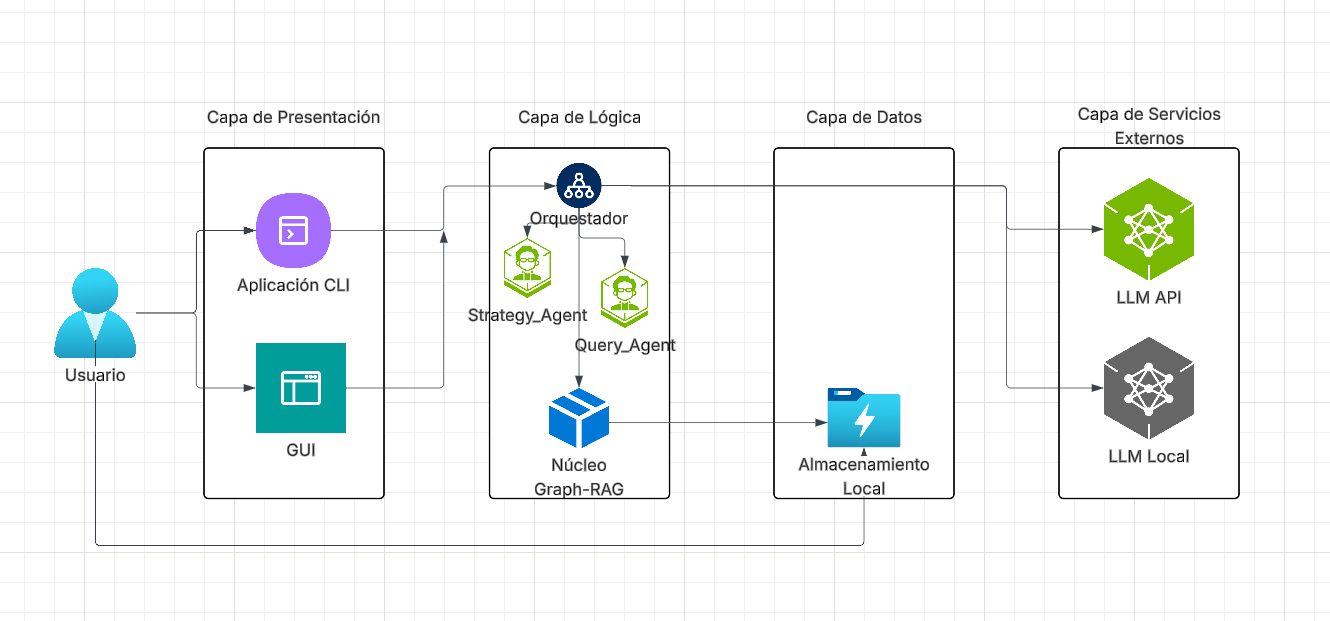
\includegraphics[width=0.9\textwidth]{images/Diagrama_Arquitectura.png}
    \caption{Diagrama de arquitectura del sistema GraphRAG desarrollado en este proyecto.}
    \label{fig:arq_intro}
\end{figure}

\vspace{0.3cm}
\textbf{Estrategias de chunking}

La forma en que se divide el documento determina la granularidad del conocimiento recuperable. Las estrategias más habituales son:

\begin{itemize}
    \item \textbf{Chunking fijo:} división por número de caracteres o tokens. Sencillo de implementar pero ignora la estructura semántica del texto, generando cortes en mitad de ideas o secciones.
    \item \textbf{Chunking con solapamiento (\textit{sliding window}):} introduce un solapamiento entre fragmentos consecutivos para preservar el contexto en los límites. Mejora la recuperación de frases cercanas a los bordes de los chunks.
    \item \textbf{Chunking jerárquico o estructural:} aprovecha la estructura del documento (índice, secciones, subsecciones) para definir las fronteras de cada fragmento. Preserva la integridad semántica de cada sección y permite reconstruir relaciones padre-hijo entre fragmentos. \textbf{Esta es la estrategia adoptada en el presente proyecto}, implementada en el módulo \texttt{chunk\_extractor.py}.
\end{itemize}

\vspace{0.3cm}
\textbf{Búsqueda híbrida: semántica y léxica}

La recuperación basada únicamente en similitud vectorial puede fallar ante términos técnicos concretos (códigos, siglas, nombres propios), ya que el embedding los ``diluye'' en el espacio semántico. Para compensarlo, este proyecto implementa una \textbf{búsqueda híbrida} que combina:

\begin{itemize}
    \item \textbf{Similitud de coseno sobre embeddings} (modelo \texttt{all-MiniLM-L6-v2} \cite{Reimers2019}): captura la intención semántica de la consulta.
    \item \textbf{BM25} (\textit{Best Matching 25}) \cite{Robertson2009}: algoritmo probabilístico de recuperación léxica que puntúa documentos en función de la frecuencia e inversión de los términos de la consulta (\textit{TF-IDF} extendido). Detecta con alta precisión términos exactos ausentes en el espacio semántico.
\end{itemize}

\vspace{0.3cm}
\textbf{Limitaciones del RAG clásico y motivación del GraphRAG}

El RAG vectorial tradicional trata cada fragmento de forma aislada, sin tener en cuenta su posición en la estructura del documento. Esto genera dos problemas recurrentes al trabajar con documentos técnicos complejos:

\begin{itemize}
    \item \textbf{Pérdida de jerarquía:} un fragmento de nivel bajo (p.ej. ``\textit{1.2.3. Requisitos de protección física}'') puede ser recuperado sin incluir el contexto de su sección padre (``\textit{1.2. Rack de comunicaciones}''), generando respuestas incompletas.
    \item \textbf{Desconexión entre secciones relacionadas:} dos secciones semánticamente relacionadas pero ubicadas en distintos capítulos no están conectadas en un sistema RAG clásico.
\end{itemize}

La solución adoptada en este proyecto, el \textbf{GraphRAG} \cite{Edge2024}, representa los fragmentos como nodos de un grafo dirigido donde las aristas codifican relaciones jerárquicas, secuenciales y semánticas entre secciones. Esto permite recuperar no solo el fragmento más relevante, sino también su contexto estructural completo, como se detalla en los capítulos de diseño e implementación.

\newpage
\subsection{Agentes y Rerankers}

\textbf{Agentes basados en LLM}

Un \textbf{agente} es un sistema que utiliza un LLM como motor de razonamiento para tomar decisiones y ejecutar acciones de forma autónoma, en función de un objetivo y del estado del entorno \cite{Yao2023}. A diferencia de una llamada directa al modelo, un agente sigue un ciclo iterativo:

\begin{enumerate}
    \item \textbf{Observación:} recibe información del entorno (consulta del usuario, metadatos del documento, resultados de búsquedas anteriores).
    \item \textbf{Razonamiento:} el LLM analiza la observación y decide la acción más adecuada.
    \item \textbf{Acción:} ejecuta la acción seleccionada (llamar a una herramienta, realizar una búsqueda, generar una respuesta).
    \item \textbf{Actualización:} el resultado de la acción se incorpora al contexto para la siguiente iteración.
\end{enumerate}

Este paradigma, popularizado por el framework \textit{ReAct} \cite{Yao2023} (Reasoning + Acting), permite construir sistemas capaces de razonar sobre cuándo y cómo utilizar herramientas externas. En el presente proyecto se implementan dos agentes especializados:

\begin{itemize}
    \item \textbf{Agente de Selección de Estrategia (\texttt{DocumentStrategyAgent}):} analiza la consulta y decide si responder con recuperación selectiva de fragmentos (\texttt{PARTIAL}) o con el documento completo (\texttt{FULL}). Esta decisión condiciona todo el flujo posterior y permite optimizar el consumo de la ventana de contexto.

    \item \textbf{Agente de Optimización de Consulta:} transforma la pregunta original del usuario, que puede contener ruido lingüístico o instrucciones de formato, en una consulta depurada centrada en los términos clave. Esto mejora la precisión de la búsqueda vectorial y léxica.
\end{itemize}

\vspace{0.3cm}
\textbf{Rerankers: bi-encoders vs cross-encoders}

En sistemas RAG, la recuperación inicial devuelve un conjunto de candidatos ordenados por similitud. Sin embargo, los modelos de embedding (\textit{bi-encoders}) calculan los vectores de consulta y documento de forma independiente, lo que introduce un margen de error en el ranking. Para refinarlo, se emplea un \textbf{reranker} basado en \textit{Cross-Encoder} \cite{Reimers2019}.

La diferencia fundamental entre ambos enfoques se resume en la siguiente tabla:

\begin{table}[H]
\centering
\renewcommand{\arraystretch}{1.4}
\caption{Comparativa entre Bi-Encoder y Cross-Encoder.}
\label{tab:biencoder_crossencoder}
\begin{tabularx}{\textwidth}{|l|X|X|}
\hline
\textbf{Característica} & \textbf{Bi-Encoder} & \textbf{Cross-Encoder} \\
\hline
\textbf{Procesamiento} & Consulta y documento codificados por separado & Consulta y documento procesados conjuntamente \\
\hline
\textbf{Velocidad} & Muy rápido (búsqueda por ANN) & Lento (requiere una pasada por par) \\
\hline
\textbf{Precisión} & Aproximada & Alta (analiza interacción directa entre términos) \\
\hline
\textbf{Uso típico} & Recuperación inicial sobre corpus grande & Reordenación (\textit{reranking}) de candidatos \\
\hline
\textbf{Modelo en este proyecto} & \texttt{all-MiniLM-L6-v2} & \nolinkurl{cross-encoder/ms-marco-MiniLM-L-6-v2} \\
\hline
\end{tabularx}
\end{table}

El flujo implementado combina ambos enfoques en dos etapas: primero, el \textit{bi-encoder} recupera eficientemente los candidatos más prometedores del grafo; después, el \textit{Cross-Encoder} reordena esos candidatos evaluando cada par (consulta, fragmento) de forma conjunta, eliminando falsos positivos semánticos y elevando al primer puesto los fragmentos que realmente responden a la pregunta.

\newpage
\subsection{Bases de Datos Vectoriales y LangGraph}

\textbf{Bases de datos vectoriales}

Una \textbf{base de datos vectorial} es un sistema de almacenamiento optimizado para indexar y consultar vectores de alta dimensión mediante búsquedas por similitud aproximada (ANN). A diferencia de las bases de datos relacionales, que buscan coincidencias exactas, las bases vectoriales permiten recuperar los elementos más próximos a un vector de consulta en el espacio de embeddings.

Las soluciones más utilizadas en el ecosistema RAG son:

\begin{table}[H]
\centering
\renewcommand{\arraystretch}{1.4}
\caption{Comparativa de bases de datos vectoriales.}
\label{tab:vectordb_intro}
\begin{tabularx}{\textwidth}{|l|X|l|}
\hline
\textbf{Solución} & \textbf{Características principales} & \textbf{Tipo} \\
\hline
FAISS & Optimizado para GPU, búsqueda en memoria, sin persistencia nativa & Open source \\
\hline
ChromaDB & Sencillo de integrar con LangChain, persistencia local & Open source \\
\hline
Pinecone & SaaS, escalabilidad gestionada, filtros por metadatos & Pago por uso \\
\hline
Weaviate & Orientado a producción, soporte multimodal & Open source / SaaS \\
\hline
\end{tabularx}
\end{table}

En el presente proyecto, dado que los documentos se procesan por sesión sin necesidad de persistencia entre ejecuciones, \textbf{no se utiliza una base de datos vectorial dedicada}. En su lugar, los embeddings se almacenan en memoria como atributos de los nodos del grafo de \texttt{NetworkX}, lo que permite integrar la búsqueda semántica directamente con el análisis estructural del documento. La incorporación de persistencia mediante ChromaDB o FAISS se propone como mejora futura en el capítulo de conclusiones.

\vspace{0.3cm}
\textbf{Grafos de conocimiento con NetworkX}

\texttt{NetworkX} es una librería de Python para la creación, manipulación y análisis de grafos y redes complejas. En este proyecto se utiliza para construir un \textbf{grafo de conocimiento dirigido} (\texttt{DiGraph}) donde:

\begin{itemize}
    \item Cada \textbf{nodo} representa una sección del documento (un \textit{chunk} jerárquico) y almacena su texto, nivel de profundidad, rango de páginas y vector de embedding.
    \item Las \textbf{aristas} codifican tres tipos de relaciones:
    \begin{itemize}
        \item \textbf{Jerárquicas:} padre $\rightarrow$ hijo, derivadas del índice del documento.
        \item \textbf{Secuenciales:} sección $\rightarrow$ sección siguiente dentro del mismo nivel.
        \item \textbf{Semánticas:} entre nodos no conectados estructuralmente cuya similitud de coseno supera un umbral predefinido ($\tau = 0.65$).
    \end{itemize}
\end{itemize}

Esta representación habilita la técnica de \textbf{propagación familiar de relevancia}: cuando un nodo obtiene una puntuación alta de similitud con la consulta, sus nodos padre, hijo y hermanos heredan parte de esa relevancia, con el objetivo de proporcionar al LLM un contexto estructural más completo que el fragmento aislado. Adicionalmente, se aplica el algoritmo \textbf{PageRank} sobre el subgrafo de consulta para identificar los nodos más centrales en términos de conectividad, complementando así la puntuación semántica.

\vspace{0.3cm}
\textbf{LangGraph para la orquestación de agentes}

\textbf{LangGraph} es una extensión del ecosistema LangChain que permite definir flujos de trabajo de agentes como grafos de estados dirigidos. Cada nodo del grafo representa una operación (llamada al LLM, herramienta externa, decisión condicional) y las aristas determinan las transiciones entre estados en función del resultado de cada nodo.

Esta arquitectura ofrece varias ventajas respecto a las cadenas lineales clásicas de LangChain:

\begin{itemize}
    \item \textbf{Ciclos y ramificaciones:} permite que el agente revise su propia decisión o realice múltiples llamadas antes de generar la respuesta final.
    \item \textbf{Estado persistente:} el grafo mantiene un estado compartido entre nodos, facilitando la transferencia de información entre etapas del pipeline.
    \item \textbf{Modularidad:} cada nodo puede ser sustituido o extendido de forma independiente sin modificar el resto del flujo.
\end{itemize}

En el sistema desarrollado, LangGraph coordina el flujo completo desde la recepción de la consulta hasta la entrega de la respuesta, conectando el agente de estrategia, el motor de recuperación sobre el grafo NetworkX y la llamada final al LLM local mediante Ollama.

\newpage
\chapter{Estado del Arte}\label{cap2}

\section{Aplicaciones empresariales de los LLMs}
Si bien el sistema desarrollado en este trabajo no es un LLM convencional, sí se apoya en ellos como motor de razonamiento, por lo que conviene analizar primero las implementaciones de uso general para avanzar después hacia las aplicaciones más específicas dentro del dominio que nos ocupa.

Dejando fuera los LLMs de propósito general empleados como asistentes virtuales generalistas (p.ej., ChatGPT, DeepSeek), se pueden señalar múltiples campos en los que los LLMs se están utilizando en entornos empresariales:

\begin{itemize}
    \item \textbf{Generación de contenido}: parcial o totalmente generado por IA. Ejemplo: en plataformas como TikTok observamos un aumento de vídeos creados casi en su totalidad mediante herramientas de IA.
    \item \textbf{Análisis de sentimientos}: análisis automatizado de reseñas o comentarios de clientes para adaptar campañas de marketing de forma más personalizada.
    \item \textbf{Sistemas de búsqueda empresarial}: asistentes capaces de responder preguntas sobre documentación corporativa extensa (manuales, normativas, contratos, informes).
\end{itemize}

Un ejemplo más próximo al objetivo de este trabajo son las soluciones de tipo \textit{document QA}, donde el usuario puede formular preguntas sobre un conjunto de documentos y recibir respuestas fundamentadas. Algunas empresas han lanzado productos en esta línea:
\begin{itemize}
    \item \textbf{Adobe}: permite consultar directamente un conjunto de PDF.
    \item \textbf{Google} y \textbf{Microsoft (Azure AI Document Intelligence)}: proponen soluciones similares basadas en técnicas de Retrieval-Augmented Generation (RAG).
\end{itemize}

El caso que merece especial atención es \textbf{AgentSet}, cuyo propósito es similar al de este trabajo. Su arquitectura se basa en RAG tradicional y no en GraphRAG. Durante la fase de investigación fue posible contactar con uno de los cofundadores, quien proporcionó información valiosa sobre cómo estructurar un proyecto de estas características.

\begin{figure}[H]
    \centering
    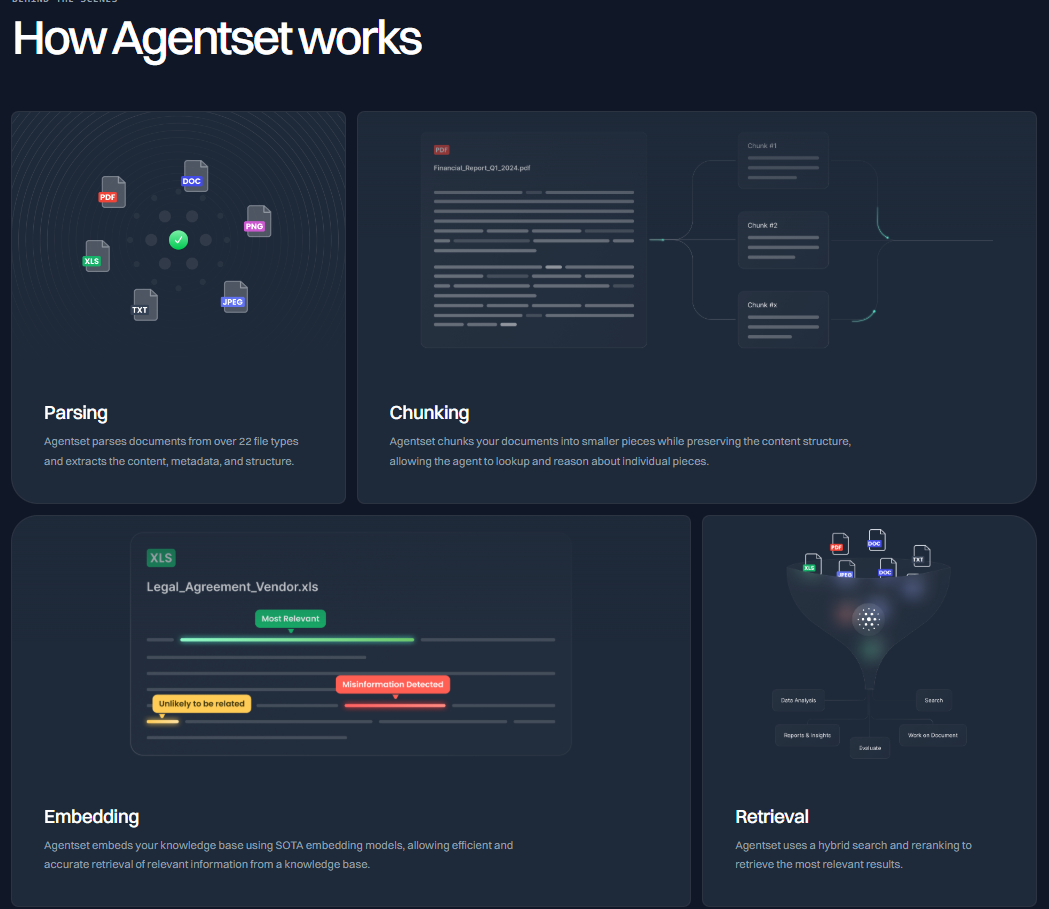
\includegraphics[width=0.8\linewidth]{images/AgentSet1.png}
    \caption{Captura de la página principal de AgentSet.}
    \label{fig:agentset}
\end{figure}

Su funcionamiento sigue un patrón ya conocido: \textit{parsing} de documentos, división en fragmentos (\textit{chunking}), generación de \textit{embeddings} y recuperación de información a partir de los mismos.  
El análisis de este y otros sistemas similares permitió identificar que no existe aún una solución empresarial ligera que funcione de manera eficiente en entornos locales sin \textit{fine-tuning}, lo cual abre la puerta a la propuesta de este trabajo.

\section{Frameworks para RAG y agentes}
La solución planteada se orienta a mejorar el rendimiento del RAG tradicional mediante técnicas avanzadas y agentes. A continuación, se presenta una comparativa de los principales frameworks empleados en proyectos de este tipo:

\begin{table}[H]
\centering
\caption{Comparativa de frameworks para RAG y agentes}
\label{tab:frameworks}
\begin{tabular}{|p{3cm}|p{4cm}|p{4cm}|p{3cm}|}
\hline
\textbf{Framework} & \textbf{Ventajas} & \textbf{Limitaciones} & \textbf{Casos de uso típicos} \\ \hline
LangChain & Amplia comunidad, gran ecosistema de integraciones & Complejidad en proyectos grandes, curva de aprendizaje elevada & Prototipado rápido, aplicaciones generales \\ \hline
LlamaIndex & Orientado a indexación y recuperación eficiente & Menor flexibilidad que LangChain & QA sobre documentos, chatbots documentales \\ \hline
LangGraph & Enfoque en agentes y grafos, facilita modularidad & Menos maduro, comunidad en crecimiento & Aplicaciones multi-agente, workflows complejos \\ \hline
Haystack & Enfoque en producción, soporta múltiples backends & Menor soporte en comunidad que LangChain & Búsqueda empresarial, pipelines NLP \\ \hline
\end{tabular}
\end{table}

Cada uno de estos frameworks presenta enfoques distintos: mientras LangChain prioriza la flexibilidad, LlamaIndex simplifica el acceso documental y LangGraph introduce el paradigma basado en grafos para mejorar el control del flujo de contexto.

\section{Bases de datos vectoriales}
Una diferencia fundamental entre implementaciones prácticas radica en cómo se almacenan y gestionan los \textit{embeddings}. Para este proyecto se analizaron las principales bases de datos vectoriales:

\begin{table}[H]
\centering
\caption{Comparativa de bases de datos vectoriales}
\label{tab:vectorDB}
\begin{tabular}{|p{3cm}|p{3cm}|p{3cm}|p{3cm}|p{3cm}|}
\hline
\textbf{Base de datos} & \textbf{Escalabilidad} & \textbf{Latencia} & \textbf{Coste} & \textbf{Integración} \\ \hline
Pinecone & Alta (SaaS, multi-región) & Baja & Pago por uso & APIs simples, integración con LangChain \\ \hline
Weaviate & Muy alta, orientada a producción & Baja & Open Source, opción SaaS & Plugins, REST/gRPC \\ \hline
FAISS & Limitada al hardware local & Muy baja (GPU optimizado) & Gratuito & Integración manual, menos amigable \\ \hline
Milvus & Escalable, soporta clusters & Media-baja & Open Source, coste en infraestructura & SDKs múltiples, alto rendimiento \\ \hline
Vespa & Altamente escalable, usado en grandes corporaciones & Media & Open Source & Más complejo de configurar \\ \hline
\end{tabular}
\end{table}

\section{Modelos de lenguaje}
No existe un único modelo estandarizado en estas aplicaciones. Según los casos analizados, se observa lo siguiente:

\begin{itemize}
    \item \textbf{Startups}: tienden a usar modelos preentrenados como ChatGPT (OpenAI) o DeepSeek, por su facilidad de integración y calidad.
    \item \textbf{Grandes empresas}: emplean modelos fine-tuneados específicamente para sus tareas, priorizando privacidad y personalización.
    \item \textbf{Modelos locales}: alternativas como LLaMA o Mistral permiten despliegues portátiles, aunque con limitaciones de rendimiento frente a modelos de API como GPT-4o o GPT-4o-mini.
\end{itemize}

De acuerdo con las pruebas realizadas, los modelos de API como ChatGPT siguen ofreciendo mejores resultados en precisión y coherencia que los modelos locales, si bien con el inconveniente del coste asociado y la dependencia de un servicio externo. En capítulos posteriores se analizan estos costes en el contexto específico del proyecto.

\section{Retos actuales y limitaciones}
A pesar del notable avance en el desarrollo y aplicación de los LLMs y sus variantes de optimización como RAG, persisten una serie de retos y limitaciones que condicionan su uso en entornos empresariales:

\begin{itemize}
    \item \textbf{Limitaciones de contexto:} aunque los modelos más recientes permiten ventanas de contexto cada vez más amplias (p.ej., GPT-4 o Claude con más de 100.000 tokens, e incluso algunos modelos experimentales con hasta un millón), la coherencia de las respuestas decae al trabajar con documentos extensos. La ampliación del contexto introduce además penalizaciones significativas en velocidad, coste y calidad de respuesta. El \textit{chunking} y la indexación no siempre garantizan una recuperación precisa; su eficacia depende del tipo de segmentación empleado y de la estructura interna de los documentos.

    \item \textbf{Alucinaciones:} los LLMs tienden a generar información inexistente o imprecisa a partir de patrones estadísticos, sin necesariamente citar fuentes verificables. En entornos regulados, esto supone riesgos legales, pérdida de confianza del usuario y costes económicos derivados de errores. Este fenómeno también puede afectar a la calidad de las respuestas en el sistema desarrollado, aunque herramientas como \textit{LettuceDetect} permiten detectar alucinaciones en las respuestas generadas.

    \item \textbf{Evaluación de resultados:} actualmente no existe un estándar robusto para medir la calidad de las respuestas, especialmente al trabajar con documentos en múltiples idiomas. Métricas como BLEU\footnote{\url{https://huggingface.co/spaces/evaluate-metric/bleu}} o ROUGE\footnote{\url{https://huggingface.co/spaces/evaluate-metric/rouge}} son útiles para evaluar la similitud léxica entre respuestas generadas y de referencia, pero no capturan la semántica ni la corrección factual. La evaluación humana, aunque más fiable, resulta subjetiva y costosa. Precisamente esta dificultad de validar respuestas automáticamente sobre documentos extensos fue uno de los detonantes del presente proyecto.

    \item \textbf{Costes computacionales:} el entrenamiento y el uso de LLMs son intensivos en recursos. Los costes asociados a las APIs comerciales (pago por token) pueden resultar prohibitivos en escenarios de gran escala, mientras que el uso de modelos locales requiere hardware dedicado con GPU de alta capacidad para obtener tiempos de respuesta aceptables.

    \item \textbf{Integración en entornos reales:} desplegar estos modelos en producción presenta retos de latencia, compatibilidad con sistemas heredados (CRMs, ERPs, bases de datos internas) y mantenimiento de \textit{pipelines} de datos. En el caso de las licitaciones públicas, la homogeneidad estructural parcial de los documentos facilita el proceso, aunque la variabilidad en formatos y codificaciones de los archivos PDF sigue representando un desafío de ingesta.
\end{itemize}

\section{Aportación del proyecto}

Del análisis precedente se desprende un ecosistema de herramientas ya consolidadas: frameworks de orquestación (LangChain, LangGraph, LlamaIndex, Haystack), bases de datos vectoriales (FAISS, ChromaDB, Pinecone, Weaviate), modelos de lenguaje locales (LLaMA, Mistral) y servicios comerciales de QA documental (Adobe, Microsoft Azure AI Document Intelligence, AgentSet). Todas estas son tecnologías existentes, no contribuciones de este trabajo. La \textbf{aportación original} reside en su combinación y adaptación específica para resolver un problema concreto —la consulta local y privada de pliegos de contratación pública— con aspectos que no están cubiertos de forma individual por ninguna de las soluciones analizadas:

\begin{itemize}
    \item \textbf{Extracción jerárquica adaptativa:} Un módulo original de segmentación de documentos PDF que reconstruye el árbol de secciones mediante hipervínculos del índice y, como mecanismo de \textit{fallback}, inferencia posicional por coordenadas X con emparejamiento difuso (\textit{fuzzy matching}). Esta lógica multiestrato, diseñada para documentos con estructuras irregulares o sin hipervínculos, no está disponible como componente reutilizable en ninguno de los frameworks analizados.

    \item \textbf{Grafo de conocimiento documental con propagación familiar de relevancia:} La representación de cada documento como un \texttt{DiGraph} de \texttt{NetworkX} con tres tipos de aristas (jerárquicas, secuenciales y semánticas) y el algoritmo de propagación familiar que eleva al Top-3 el 95\,\% de los fragmentos que el RAG vectorial puro deja fuera del Top-5. Esta capacidad de recuperar contexto estructural completo (padre $\rightarrow$ hijo) no es inherente a ninguno de los frameworks de RAG convencionales.

    \item \textbf{Agente de selección de estrategia de recuperación:} Un agente LLM especializado que clasifica cada consulta como \texttt{PARTIAL} (recuperación selectiva de fragmentos) o \texttt{FULL} (contexto completo del documento), con una tasa de acierto del 96\,\% demostrada experimentalmente. Esta decisión dinámica y adaptativa al dominio específico no es un componente estándar de los pipelines RAG analizados.

    \item \textbf{Despliegue completamente local y privado:} La integración de todos los componentes —embeddings, reranker, LLM, agentes— en un pipeline ejecutable sin conexión a internet, sin \textit{fine-tuning} ni reentrenamiento, adecuado para documentos con requisitos de confidencialidad. Esto contrasta directamente con soluciones como AgentSet, que procesa los documentos en servidores externos.

    \item \textbf{Validación empírica cuantitativa en dominio específico:} Un protocolo de evaluación con métricas automáticas (Token F1, ROUGE-L, BERTScore, RAGAS) y un estudio de ablación por componentes sobre 30 preguntas con \textit{ground truth} definido, que permite aislar y cuantificar la contribución individual de cada módulo del sistema.
\end{itemize}

En contraste con los sistemas analizados, que priorizan la escalabilidad o la facilidad de integración en arquitecturas de nube, la propuesta de este trabajo prioriza la preservación de la jerarquía documental, la soberanía del dato y la viabilidad en hardware de usuario sin modificación de modelos base.

\chapter{Motivación}\label{cap3}

En este capítulo se presentan las razones que justifican la creación de este proyecto, cuáles son sus objetivos, las etapas de desarrollo y otros datos relevantes como una estimación de presupuesto, considerando tanto el desarrollo como la puesta en práctica en un caso concreto.

Los LLMs fueron introduciéndose paulatinamente en mi vida —y posiblemente en la de cualquier estudiante—. Eran capaces de resolver dudas que un usuario podría tardar mucho tiempo en responder, generar resúmenes de contenido e incluso formular preguntas sobre el mismo. Todo ello representaba un gran valor. Sin embargo, en muchas ocasiones surgía un problema recurrente: cuando un documento era demasiado extenso, introducirlo completo en el modelo no era posible por limitaciones de contexto, y dividirlo manualmente resultaba ineficiente. El resultado eran respuestas imprecisas o incompletas.

Esta situación despertó la curiosidad por entender cómo funcionaban estos modelos y si dicho problema era realmente solucionable. En paralelo, el uso de los LLMs se expandía rápidamente entre el público general, generando un mercado cada vez más relevante. La investigación realizada permitió comprobar que, lejos de estar resuelto, se trataba de un desafío en plena evolución.

La oportunidad se concretó cuando, durante el período de prácticas en la empresa, se planteó un reto similar: trabajar con documentos de gran extensión —en concreto, licitaciones públicas— optimizando la recuperación de información y las respuestas generadas, con el objetivo de facilitar la elaboración de las memorias técnicas necesarias para concurrir a dichos procesos. El beneficio económico derivado del ahorro de tiempo del personal resultó evidente.  

En resumen, la motivación detrás de este proyecto responde a tres ejes principales:  
\begin{itemize}
    \item \textbf{Científico}: explorar y aplicar soluciones innovadoras en torno al uso de LLM en documentos extensos.  
    \item \textbf{Económico}: demostrar el potencial de ahorro de costes y optimización de procesos en entornos empresariales.  
    \item \textbf{Personal}: adquirir un conocimiento profundo de estas tecnologías y afrontar un reto de alto interés práctico.  
\end{itemize}

\section{Objetivos y etapas del proyecto}
\subsection{Objetivos}
Los principales objetivos del proyecto son:  
\begin{itemize}
    \item Desarrollar una solución personalizada al problema del contexto en los LLMs en documentos extensos, como licitaciones públicas.
    \item Comprender cómo funciona un LLM a nivel interno.
    \item Aprender y aplicar las últimas tecnologías en uso en el sector.
    \item Diseñar un sistema propio de segmentación de documentos (chunking), distinto a los clásicos.
    \item Entender y profundizar en el uso de agentes, sus librerías y aplicaciones.
    \item Explorar soluciones alternativas a las vistas en el Estado del Arte.
\end{itemize}

\subsection{Etapas}
El desarrollo del proyecto se organizó en las siguientes fases:  
\begin{itemize}
    \item \textbf{Investigación}: etapa inicial de gran importancia. Si bien contaba con conocimientos básicos, profundicé en los fundamentos: qué es un LLM, cómo funcionan los transformadores, la tokenización, etc. Posteriormente, la investigación se centró en técnicas para alimentar al modelo con información contextualizada, como RAG y GraphRAG. Para ello se emplearon fuentes diversas, desde foros oficiales hasta tutoriales prácticos.  
    \item \textbf{Diseño}: desde un inicio se optó por una arquitectura en tres capas:  
        \begin{enumerate}
            \item Capa de agentes, responsables de la toma de decisiones.  
            \item Capa de segmentación de documentos, encargada de dividir en chunks limpios y eficientes en número de tokens.  
            \item Capa de lógica del modelo, que realiza las ponderaciones y devuelve al usuario una respuesta coherente y fundamentada.  
        \end{enumerate}
    \item \textbf{Implementación}: se afrontaron retos técnicos como incompatibilidades entre librerías, pruebas con diferentes métodos y las imprecisiones frecuentes en modelos locales.  
    \item \textbf{Validación}: se realizaron pruebas sobre el \textit{dataset} de documentos descrito en el Capítulo~\ref{cap7}, combinando un estudio de ablación por componentes con la métrica de precisión de recuperación P@3 sobre un conjunto de 30 preguntas con respuesta de referencia conocida. En el entorno empresarial se empleó adicionalmente la herramienta \textit{LettuceDetect} para la detección de alucinaciones en las respuestas generadas, así como validaciones empíricas con casos de uso reales.
\end{itemize}

\section{Recursos utilizados}
Para el desarrollo del proyecto se emplearon los siguientes recursos:  

\begin{itemize}
    \item \textbf{Software}: se utilizó Python como lenguaje de programación, junto con librerías clave como:
    \begin{itemize}
        \item \texttt{rank\_bm25} (BM25Okapi) para recuperación de información.  
        \item \texttt{networkx} para la representación y manipulación de grafos.  
        \item \texttt{matplotlib} para la visualización.  
        \item \texttt{sentence\_transformers} y \texttt{scikit-learn} para embeddings y métricas de similitud.  
        \item \texttt{ollama} y \texttt{tiktoken} para la gestión de modelos y conteo de tokens.  
        \item \texttt{thefuzz} para comparación de cadenas.  
        \item \texttt{langchain} y \texttt{CrossEncoder} para operaciones avanzadas en RAG.  .  
    \end{itemize}

    \item \textbf{Hardware}: se trabajó principalmente en un portátil proporcionado por la empresa (MSI Cyborg, 32 GB RAM y GPU dedicada), que, si bien es un dispositivo portátil, permite ejecutar modelos locales de hasta 8--13B parámetros con aceleración CUDA.

    \item \textbf{Recursos humanos}: el trabajo fue realizado de manera individual, con el apoyo de un \textit{Senior} con conocimientos en IA, con reuniones casi diarias para la supervisión y resolución de problemas.  
\end{itemize}

\section{Caso de negocio}
Este apartado expone la aplicabilidad y justificación del proyecto en un entorno real.  

\subsection{Agentes implicados en el proyecto}
\begin{itemize}
    \item \textbf{Beneficiarios directos}: la empresa en la que se desarrolló el proyecto, al mejorar la eficiencia en el manejo de documentos extensos como licitaciones públicas. Su implementación se encuentra en fase de piloto, prevista para su puesta en producción una vez se reactive el mercado de consultoría tras el período estival.
    \item \textbf{Usuarios finales}: personal de la empresa que necesita consultar información en grandes volúmenes de texto y elaborar las memorias técnicas para concurrir a licitaciones, así como cualquier otro rol que pudiera beneficiarse de una herramienta de consulta documental.
    \item \textbf{Otros interesados}: investigadores interesados en la optimización de sistemas RAG y en el uso de GraphRAG como enfoque alternativo, así como potenciales clientes de sectores con necesidades documentales similares.
\end{itemize}

\subsection{Presupuesto}
La siguiente tabla resume una estimación de los costes asociados al proyecto:

\begin{table}[H]
\centering
\small
\begin{tabularx}{\textwidth}{|l|c|>{\raggedright\arraybackslash}X|}
\hline
\textbf{Concepto} & \textbf{Coste estimado (€)} & \textbf{Observaciones} \\ \hline
Hardware (portátil) & 1.200 & Proporcionado por la empresa \\ \hline
Software & 200 & Librerías open source, salvo costes puntuales \\ \hline
Horas de trabajo (160 h aprox.) & 2.660 & 20 h/semana durante 2 meses, tarifa Junior (Usando el coste a la empresa, no lo que cobra el trabajador) \\ \hline
Costes adicionales (cloud, API) & 0,50 & Cada consulta +- 0,01 €, uso puntual \\ \hline
\textbf{Total estimado} & \textbf{4.060,50} &  \\ \hline
\end{tabularx}
\caption{Estimación de presupuesto del proyecto.}
\label{tab:presupuesto}
\end{table}

Se entrará más en los gastos de la API en el capítulo de implementación, pero muchas de las consultas no superaban el céntimo de euro por petición.  
En cuanto a las horas de trabajo, el coste se estimó a partir de las horas invertidas (20 semanales durante aproximadamente 2 meses) y multiplicado por un sueldo estándar de \textit{Developer Junior} en coste a la empresa. Este cálculo es meramente orientativo, ya que una persona trabajando a jornada completa y con mayor experiencia podría reducir los tiempos y, por tanto, los costes, en función del nivel salarial correspondiente.


\begin{table}[H]
\centering
\begin{tabularx}{\textwidth}{|l|X|X|}
\hline
\textbf{Concepto} & \textbf{Coste mensual estimado (€)} & \textbf{Observaciones} \\ \hline
Servidor físico (GPU 24--48 GB VRAM, 128 GB RAM) & 4.800 & Precio de adquisición, amortizado a 3 años \\ \hline
Electricidad & 120 & Consumo medio 400 W en uso continuo \\ \hline
Mantenimiento (hardware/software) & 50 & Reemplazos, soporte, licencias menores \\ \hline
\textbf{Total mensual} & \textbf{500} & Incluye amortización del hardware \\ \hline
\end{tabularx}
\caption{Estimación de costes mensuales para mantener un servidor con un modelo LLM local.}
\label{tab:servidor}
\end{table}

En este cálculo se supone la adquisición de una máquina capaz de albergar un modelo de entre 7B y 13B parámetros (ej. NVIDIA RTX A6000 o similar con 48 GB de VRAM). Se amortiza el coste del hardware (aprox. 4.800 €) en un periodo de 3 años, resultando unos 400 € mensuales.  
A esto se añade el coste eléctrico (400 W de consumo medio, 24/7, con un precio aproximado de 0,25 €/kWh) y una partida para mantenimiento preventivo y correctivo.  
El coste total mensual ronda los \textbf{500 €}, lo cual permite comparar la viabilidad frente a soluciones en la nube. Nótese que, según las pruebas realizadas, es posible que se requieran modelos con más parámetros para casos de uso más exigentes, lo que incrementaría el coste. De nuevo, este cálculo es meramente orientativo.



\subsection{Impacto}
El impacto del proyecto puede resumirse en los siguientes puntos:  
\begin{itemize}
    \item \textbf{Productividad}: reducción significativa del tiempo necesario para consultar documentos extensos.  
    \item \textbf{Eficiencia}: posibilidad de automatizar tareas de análisis documental, liberando recursos humanos para labores de mayor valor añadido.  
    \item \textbf{Aplicaciones futuras}: escalabilidad hacia otros tipos de documentos o incluso integración con sistemas empresariales más amplios.  
    \item \textbf{Impacto académico}: contribución al estudio de técnicas alternativas al RAG tradicional, con valor tanto práctico como científico.  
\end{itemize}

      \chapter{Análisis de Requisitos}
\label{chap:requisitos}

En este capítulo se establecen los requisitos que la solución de software propuesta debe satisfacer. Estos se dividen en dos categorías principales: los requisitos funcionales, que describen las funcionalidades y capacidades que el sistema debe ofrecer (el <<qué>>), y los requisitos no funcionales, que definen los atributos de calidad, restricciones y características operativas del sistema (el <<cómo de bien>>).

\section{Requisitos Funcionales (RF)}
\label{sec:rf}

Los requisitos funcionales del sistema se han agrupado en tres categorías principales que se corresponden con las fases lógicas del flujo de trabajo: (1) Ingesta y Procesamiento Estructural de los Documentos; (2) Representación y Enriquecimiento del Conocimiento; y (3) Interacción, Búsqueda y Generación de Respuestas. A continuación, se detalla cada grupo en tablas separadas.
\newpage
\subsubsection*{Grupo 1: Ingesta y Procesamiento Estructural de Documentos}
Estos requisitos describen las funcionalidades necesarias para cargar, analizar y segmentar los documentos de entrada, transformando el contenido no estructurado en una representación jerárquica inicial.

\begin{table}[H]
\centering
\renewcommand{\arraystretch}{1.4} % Aumenta el espacio vertical para mejorar la legibilidad
\caption{Requisitos Funcionales: Ingesta y Procesamiento Estructural.}
\label{tab:rf_ingesta}
\begin{tabularx}{\textwidth}{|l|l|X|}
\hline
\textbf{ID} & \textbf{Nombre} & \textbf{Descripción} \\
\hline
\textbf{RF-01} & Carga de Documentos & El sistema deberá permitir la carga simultánea de múltiples documentos en formato PDF desde una ruta de directorio especificada. \\
\hline
\textbf{RF-02} & Detección Adaptativa de TOC & El sistema deberá implementar una estrategia dual para detectar la Tabla de Contenidos (TOC): prioritariamente mediante el análisis de hipervínculos internos y, como alternativa, mediante el reconocimiento de patrones textuales con expresiones regulares. \\
\hline
\textbf{RF-03} & Inferencia de Jerarquía & El sistema deberá construir una estructura jerárquica (padre-hijo) de las secciones del documento, basándose en el análisis de prefijos numéricos (ej: 1.2.1) y la indentación visual (posición X) de los títulos en la TOC. \\
\hline
\textbf{RF-04} & Chunking Jerárquico & El sistema deberá segmentar (chunking) los documentos de forma estructural, creando chunks cuyo contenido corresponde al texto delimitado entre el título de una sección y el de la siguiente, localizando dichos títulos con precisión mediante similitud difusa (fuzzy matching). \\
\hline
\end{tabularx}
\end{table}

\newpage
\subsubsection*{Grupo 2: Representación y Enriquecimiento del Conocimiento}
Una vez procesada la estructura inicial, los siguientes requisitos se centran en cómo esta información es representada, almacenada y enriquecida semánticamente para facilitar una recuperación de información más avanzada.

\begin{table}[H]
\centering
\renewcommand{\arraystretch}{1.4}
\caption{Requisitos Funcionales: Representación y Enriquecimiento.}
\label{tab:rf_representacion}
\begin{tabularx}{\textwidth}{|l|l|X|}
\hline
\textbf{ID} & \textbf{Nombre} & \textbf{Descripción} \\
\hline
\textbf{RF-05} & Construcción de Grafo Estructural & Cada documento deberá ser representado como un grafo dirigido (\texttt{NetworkX}), donde los nodos son los chunks y las aristas representan relaciones estructurales (jerárquicas y secuenciales). \\
\hline
\textbf{RF-06} & Enriquecimiento Semántico del Grafo & El grafo estructural deberá ser enriquecido mediante la adición de aristas semánticas entre nodos no conectados estructuralmente que superen un umbral predefinido de similitud de coseno entre sus embeddings. \\
\hline
\textbf{RF-07} & Generación de Embeddings Duales & Para cada chunk, el sistema deberá generar y almacenar dos representaciones vectoriales (embeddings) distintas: una para su título y otra para su contenido textual. \\
\hline
\end{tabularx}
\end{table}

\newpage
\subsubsection*{Grupo 3: Interacción, Búsqueda y Generación (GraphRAG)}
Este grupo final de requisitos define el núcleo interactivo del sistema, detallando cómo se procesa la consulta del usuario, se recupera la información relevante del grafo de conocimiento y se genera la respuesta final.

\begin{table}[H]
\centering
\renewcommand{\arraystretch}{1.4}
\caption{Requisitos Funcionales: Interacción, Búsqueda y Generación.}
\label{tab:rf_interaccion}
\begin{tabularx}{\textwidth}{|l|l|X|}
\hline
\textbf{ID} & \textbf{Nombre} & \textbf{Descripción} \\
\hline
\textbf{RF-08} & Selección de Estrategia por Agente & Un agente basado en LLM deberá analizar la consulta del usuario para determinar la estrategia de respuesta óptima: Acceso Parcial (RAG) para preguntas específicas, o Acceso Completo para preguntas generales (ej: resúmenes). \\
\hline
\textbf{RF-09} & Optimización de Consulta por Agente & Un agente LLM deberá refinar la consulta del usuario antes de la búsqueda, simplificándola a sus términos clave para mejorar la precisión del sistema de recuperación de información. \\
\hline
\textbf{RF-10} & Búsqueda Híbrida y Re-ranking & El sistema realizará una búsqueda híbrida combinando similitud semántica (embeddings) y búsqueda lexicográfica (BM25) sobre sub-chunks. Los resultados serán reordenados mediante un modelo Cross-Encoder para maximizar la relevancia. \\
\hline
\textbf{RF-11} & Selección de Contexto Basada en Grafo & El contexto final se seleccionará analizando un subgrafo de consulta, aplicando una puntuación final a cada nodo que combina su relevancia directa, la relevancia propagada de sus familiares (padre, hijos, hermanos) y métricas de centralidad del grafo. \\
\hline
\textbf{RF-12} & Modos de Respuesta Múltiples & El sistema deberá ser capaz de generar respuestas en dos modos: individual (una respuesta por documento) y consolidado (una única respuesta sintetizada a partir de todos los documentos). \\
\hline
\end{tabularx}
\end{table}
\newpage

\section{Requisitos No Funcionales (RNF)}
\label{sec:rnf}

Los requisitos no funcionales definen los atributos de calidad del sistema, tales como su rendimiento, modularidad, robustez y mantenibilidad. Estos requisitos son cruciales para asegurar que el sistema no solo funcione, sino que lo haga de manera eficiente y fiable. A continuación, se detallan agrupados por su naturaleza.

\subsubsection*{Grupo 1: Atributos de Arquitectura y Calidad de Software}
Este grupo define las características intrínsecas del diseño y la construcción del software que garantizan su mantenibilidad, flexibilidad y adaptabilidad a futuro.

\begin{table}[H]
\centering
\renewcommand{\arraystretch}{1.4}
\caption{Requisitos No Funcionales: Arquitectura y Calidad.}
\label{tab:rnf_arquitectura}
\begin{tabularx}{\textwidth}{|l|l|X|}
\hline
\textbf{ID} & \textbf{Nombre} & \textbf{Descripción} \\
\hline
\textbf{RNF-01} & Modularidad & La arquitectura del sistema deberá estar desacoplada, con una clara separación de responsabilidades entre los componentes de extracción (\texttt{chunk\_extractor.py}), decisión (\texttt{document\_strategy\_agent.py}) y el núcleo RAG (\texttt{main.py}), facilitando su mantenimiento y escalabilidad. \\
\hline
\textbf{RNF-02} & Configurabilidad & El sistema deberá permitir la configuración del modelo de lenguaje (LLM) a utilizar a través de parámetros, sin necesidad de modificar el código fuente principal. \\
\hline
\textbf{RNF-03} & Portabilidad (Ejecución Local) & El sistema deberá ser capaz de operar utilizando modelos de lenguaje alojados localmente mediante una interfaz como Ollama, garantizando su funcionamiento sin dependencia de servicios cloud de pago. \\
\hline
\end{tabularx}
\end{table}

\newpage
\subsubsection*{Grupo 2: Atributos de Operación y Rendimiento}
Estos requisitos se centran en el comportamiento observable del sistema durante su ejecución, incluyendo su eficiencia, fiabilidad y la facilidad para diagnosticar su funcionamiento.

\begin{table}[H]
\centering
\renewcommand{\arraystretch}{1.4}
\caption{Requisitos No Funcionales: Operación y Rendimiento.}
\label{tab:rnf_operacion}
\begin{tabularx}{\textwidth}{|l|l|X|}
\hline
\textbf{ID} & \textbf{Nombre} & \textbf{Descripción} \\
\hline
\textbf{RNF-04} & Trazabilidad y Depuración & El sistema deberá generar artefactos para la depuración, incluyendo visualizaciones del grafo de consulta (\texttt{.png}) y archivos de texto (\texttt{.txt}) que registren el contexto exacto enviado al LLM en cada consulta. \\
\hline
\textbf{RNF-05} & Robustez & El sistema deberá gestionar de forma controlada los errores durante la lectura de documentos (ej: PDFs corruptos), notificando al usuario y continuando la operación con los archivos válidos sin interrumpir la ejecución. \\
\hline
\textbf{RNF-06} & Gestión de Recursos & La versión del sistema que opera con modelos locales deberá ser funcional en equipos de escritorio con especificaciones de hardware razonables (ej: 16 GB de RAM y GPU con 8 GB de VRAM). \\
\hline
\end{tabularx}
\end{table}

      \chapter{Metodología y Diseño de la Solución}\label{cap5}

\section{Metodología de desarrollo}
\label{sec:metodologia}

Para la planificación y ejecución de este Trabajo de Fin de Grado, se ha adoptado una \textbf{metodología de desarrollo iterativa e incremental}, inspirada en los principios ágiles. Esta elección se fundamenta en la naturaleza del proyecto, que combina la investigación de tecnologías emergentes (sistemas GraphRAG, agentes LLM) con la construcción de un prototipo de software funcional. A diferencia de un modelo en cascada, este enfoque se adapta a la naturaleza exploratoria del trabajo, permitiendo construir el sistema en ciclos cortos donde cada iteración produce un incremento funcional, ofreciendo ventajas clave como la flexibilidad, la gestión de la incertidumbre y la entrega de valor temprana.
La necesidad de cambios constantes a lo largo del proyecto validó esta elección: al incorporar una componente de investigación, al inicio no existía una visión completamente definida de la versión final, y los ciclos de prueba, error y aprendizaje permitieron ir modelando el sistema de forma incremental.


\newpage
\subsection{Fases del Proyecto}
El desarrollo del proyecto se estructuró en cinco fases lógicas, que se alinean con los capítulos de esta memoria y cuyo cronograma se detalla en la Tabla~\ref{tab:cronograma}. Las semanas concretas son orientativas; así, por ejemplo, la investigación se prolongó a lo largo de todo el proyecto, especialmente al término de cada iteración, con el fin de identificar mejoras sobre la base ya obtenida.

\begin{description}
    \item[Fase 1: Investigación y Definición (Semanas 1-4).] Se realizó una revisión bibliográfica exhaustiva, se definieron los objetivos del proyecto y se identificaron las tecnologías clave (Ollama, NetworkX, etc.).
    \item[Fase 2: Análisis y Diseño (Semanas 5-7).] Se formalizaron los requisitos funcionales (RF) y no funcionales (RNF), se diseñó la arquitectura general de la solución y se definieron los componentes principales del sistema.
    \item[Fase 3: Desarrollo Incremental (Semanas 8-12).] Núcleo del trabajo práctico, subdividido en tres incrementos funcionales que se detallan en el Anexo \ref{anexo:planificacion}:
        \begin{enumerate}
            \item \textbf{Incremento 1 (MVP - Núcleo RAG):} Desarrollo del pipeline de ingesta, chunking jerárquico y RAG básico para un solo documento.
            \item \textbf{Incremento 2 (Sofisticación con Grafo):} Implementación del grafo estructural y semántico, búsqueda híbrida y re-ranking.
            \item \textbf{Incremento 3 (Inteligencia de Agentes):} Integración de los agentes para optimización de consultas y selección de estrategia, y soporte para múltiples documentos.
        \end{enumerate}
    \item[Fase 4: Pruebas y Evaluación (Semanas 13-14).] Verificación del cumplimiento de los requisitos y evaluación de la calidad de las respuestas del sistema.
    \item[Fase 5: Documentación (Semanas 15-16).] Redacción final de esta memoria y preparación de la defensa.
\end{description}

\newpage
A continuación se presenta un resumen del cronograma, expresando de manera aproximada la carga de trabajo en cada una de las fases del proyecto. Si bien en la práctica el desarrollo resultó más complejo que lo recogido en la tabla, esta ofrece una síntesis representativa del mismo.
\begin{table}[H]
    \centering
    \renewcommand{\arraystretch}{1.3}
    \caption{Cronograma de Fases e Hitos Principales del Proyecto.}
    \label{tab:cronograma}
    \begin{tabularx}{\textwidth}{|l|l|X|}
    \hline
    \textbf{Fase} & \textbf{Semanas} & \textbf{Hitos y Entregables Clave} \\
    \hline
    \textbf{1. Investigación y Definición} & 1 - 4 & Objetivos definidos. Estado del arte completado. Tecnologías seleccionadas. \\
    \hline
    \textbf{2. Análisis y Diseño} & 5 - 7 & Documento de requisitos (Cap. 2). Diseño de arquitectura y componentes (Cap. 3). \\
    \hline
    \textbf{3. Desarrollo Incremental} & 8 - 12 & Código fuente de los tres incrementos funcionales completado. Ver Anexo \ref{anexo:planificacion} para el detalle de las tareas. \\
    \hline
    \textbf{4. Pruebas y Evaluación} & 13 - 14 & Plan de pruebas ejecutado. Análisis de resultados cualitativos y cuantitativos. \\
    \hline
    \textbf{5. Documentación} & 15 - 16 & Redacción y entrega de la memoria final del TFG. \\
    \hline
    \end{tabularx}
\end{table}

\newpage
\subsection{Herramientas de Apoyo a la Metodología}
Para la gestión eficaz de este proceso, se utilizaron herramientas estándar en la industria del desarrollo de software.

\subsubsection{Control de Versiones con Git}
El código fuente del proyecto se gestionó en una rama privada, dado que parte de sus contenidos podría ser confidencial para la empresa, como ocurre con algunos documentos de prueba. La rama de trabajo no puede adjuntarse públicamente; en su lugar, se ha habilitado una rama con documentos de origen público que reproduce la misma estructura. El modelo de ramificación empleado fue muy sencillo y constaba de los siguientes elementos:
\begin{itemize}
    \item \texttt{main}: Rama principal que contiene siempre la versión más estable y funcional del código. En concreto, todas las ramas se integraban una vez por incremento para verificar que las funcionalidades operasen conjuntamente de forma correcta.
    \item \texttt{feature/nombre-tarea}: Ramas de corta duración creadas para desarrollar una nueva funcionalidad o corregir un error. Una vez completada y probada, la rama se fusionaba con \texttt{main}; en la mayoría de los casos se creaba una rama por cada requisito funcional.
\end{itemize}
El uso de mensajes de commit descriptivos aseguró la trazabilidad de cada cambio realizado en el código.

\subsubsection{Gestión de Tareas con Kanban}
El seguimiento de las tareas de cada incremento se realizó mediante un tablero \textbf{Kanban} en la herramienta Trello. El tablero se estructuró en cuatro columnas principales: \textit{Backlog}, \textit{Pendiente (To Do)}, \textit{En Progreso (In Progress)} y \textit{Finalizado (Done)}. Este enfoque visual permitió priorizar el trabajo, limitar el trabajo en curso a una o dos tareas simultáneamente para mantener el foco, y tener una visión clara del progreso. En el \textbf{Anexo \ref{anexo:kanban}} se presentan capturas de pantalla del estado del tablero al finalizar cada incremento.

\subsection{Definición de Terminado (Definition of Done)}
Para asegurar la calidad y consistencia del trabajo en cada incremento, se estableció una "Definición de Terminado" (Definition of Done). Una tarea no se consideraba finalizada hasta que cumplía con todos los siguientes criterios:
\begin{itemize}
    \item El código asociado a la funcionalidad está implementado y cumple con los requisitos.
    \item El código ha sido auto-revisado y refactorizado para asegurar su legibilidad, con los comentarios correspondientes en aquellas funcionalidades que pudiesen llegar a causar confusión.
    \item Se han realizado pruebas unitarias o de integración informales para verificar que la nueva funcionalidad no introduce regresiones.
    \item El código ha sido fusionado (\textit{merged}) a la rama \texttt{main} del repositorio Git.
    \item La tarjeta correspondiente en el tablero Kanban ha sido movida a la columna \textit{Finalizado (Done)}.
\end{itemize}

Todas estas medidas, en especial el control de versiones con Git y el tablero Kanban, resultaron fundamentales para no perder tiempo identificando cuál era la siguiente tarea, además de facilitar la reversión de cambios de forma sencilla.

\newpage
\section{Arquitectura general de la solución}
\subsection{Arquitectura y Diseño del Sistema}

Para la construcción de esta solución se barajaron una serie de patrones. Finalmente, se optó por un patrón de \textbf{Arquitectura en capas}.
La elección se fundamenta en la propia necesidad de separación de las distintas responsabilidades del sistema, en específico aportando una modularidad al mismo.

Por ejemplo, al cambiar del uso de un modelo local al de una API de pago (GPT-4o-mini en las pruebas de evaluación), únicamente fue necesario modificar un único módulo, gracias a dicha modularidad.
La mantenibilidad también mejora por el mismo motivo: ante cualquier cambio, no es necesario modificar la totalidad de los módulos.
La cohesión, al tener los componentes separados, permite una comprensión más clara del sistema, sin necesidad de recorrer un único fichero de miles de líneas en busca de una funcionalidad concreta.

\subsection{Capas de la Arquitectura}

La Arquitectura de este sistema se organiza en \textbf{cuatro capas}:

\subsubsection{Capa de Presentación}

En este caso, mediante una interfaz \textbf{CLI} (también se probaron interfaces sencillas con Gradio).
Cuando se probó a implementar con GUI, esta se mantuvo en su propio documento.
Para mantenerlo sencillo con CLI, se implementa en la función \texttt{interactive\_chat()}, que es el punto de entrada desde el cual el usuario puede comunicarse con el resto de la aplicación.

\subsubsection{Capa de Lógica}

Es el corazón del sistema.
Dado que la lógica es compleja, está separada en distintos documentos. En concreto:

\paragraph{Orquestador Inteligente (\texttt{SmartDocumentProcessor}):}
Este es el componente central.
Recibe la consulta del usuario y dirige todo el flujo de la misma hasta la obtención de la respuesta.

\paragraph{Agentes:}
\begin{itemize}
    \item \textbf{Agente de Estrategia (\texttt{DocumentStrategyAgent}):}
    Es un subcomponente llamado por el orquestador.
    Su tarea es, a partir de la \textit{query} realizada por el usuario, decidir si utilizar partes del documento (empleando GraphRAG) o si, por el contrario, la pregunta requiere necesariamente de un contexto completo, como puede ser un resumen del mismo.

    \item \textbf{Agente de Optimización de Consulta (\texttt{DocumentStrategyAgent}):}
    Subcomponente llamado por el orquestador cuya tarea es refinar la consulta del usuario.
    Se explicará con más detalle en su respectivo punto, pero resumidamente formula una pregunta más apta para la búsqueda con GraphRAG, en caso de que el Agente de Estrategia haya decidido esa ruta.
\end{itemize}

\paragraph{Núcleo GraphRAG (\texttt{PDFRAGSystemWithNetworkX}):}
Es el principal motor de la búsqueda, análisis del grafo, generación del contexto que se dará al LLM y creación de la respuesta generada para el usuario.

\subsubsection{Capa de Datos}

En este caso, al no trabajar con documentos recurrentes, no se mantiene persistencia de los \textit{embeddings} fuera de la ejecución.
(Es una de las propuestas futuras que depende exclusivamente de las necesidades del usuario).

Por tanto, al momento de la entrega, la capa de datos es únicamente el sistema de ficheros en el que se almacena el grupo de documentos con el que alimentar al LLM a la hora de proporcionarle contexto.

\subsubsection{Servicios Externos}

Dependiendo de las necesidades de la implementación concreta:

\begin{itemize}
    \item \textbf{LLM Local:}
    Utiliza un servicio como \textit{Ollama}, que escucha peticiones HTTP y es capaz de devolver respuestas generadas localmente.
    Al recibir una petición, el servicio ejecuta el modelo en la máquina del usuario, procesa la entrada y devuelve la respuesta correspondiente.

    \item \textbf{API Externa:}
    Se emplea un cliente de API externa para conectarse a otro proveedor (por ejemplo, GPT u otro).
    Es más sencillo de desplegar y evita los problemas de albergar un servidor localmente, aunque conlleva un coste en función del uso.
\end{itemize}

\subsection{Conclusión}

Esta estructura permite que cada uno de los componentes se centre en una tarea específica y, por tanto, lograr la \textbf{modularidad} establecida en el RNF-01, además del resto de ventajas anteriormente mencionadas.


\section{Casos de uso}

\newpage
\subsection{CU-01 Subida de Documentos}
\begin{table}[H]
\centering
\renewcommand{\arraystretch}{1.3} % más espacio entre filas
\begin{tabularx}{\textwidth}{|l|X|}
\hline
\textbf{Identificador} & CU-01 \\
\hline
\textbf{Nombre} & Subida de Documentos \\
\hline
\textbf{Objetivo} & Determinar si el documento que proporciona el usuario es de un tipo válido. \\
\hline
\textbf{Actores} & Principal: Usuario \\
\hline
\textbf{Precondiciones} & Debe de tenerse uno o varios archivos en formato texto. \\
\hline
\textbf{Disparador (Trigger)} & Introducir el documento o bien en la carpeta destinada, o al ejecutarlo en GUI en el TextBox. \\
\hline
\textbf{Flujo principal} &
1. Introducción del documento. \newline
2. Éxito. \newline
3. Error, documento no válido. \\
\hline
\textbf{Flujos alternativos} & No. \\
\hline
\textbf{Excepciones} & E1: Error de características (Tamaño...). \newline E2: Error de Formato (Intentar introducir un .zip, .mp4...). \\
\hline
\textbf{Postcondiciones} & El sistema obtiene los documentos. \\
\hline
\textbf{Entradas} & Documentos (Sin limite aparente de los mismos), en formatos aceptados por los extractores de texto, .pdf, .docx... , y con un tamaño total inferior a 500mb. \\
\hline
\textbf{Salidas} & Documentos con formato comprobado. \\
\hline
\textbf{Prioridad / Frecuencia} & Alta. \\
\hline
\end{tabularx}
\caption{Ficha del caso de uso CU-01.}
\label{tab:CU-01}
\end{table}

\begin{figure}[H]
    \centering
    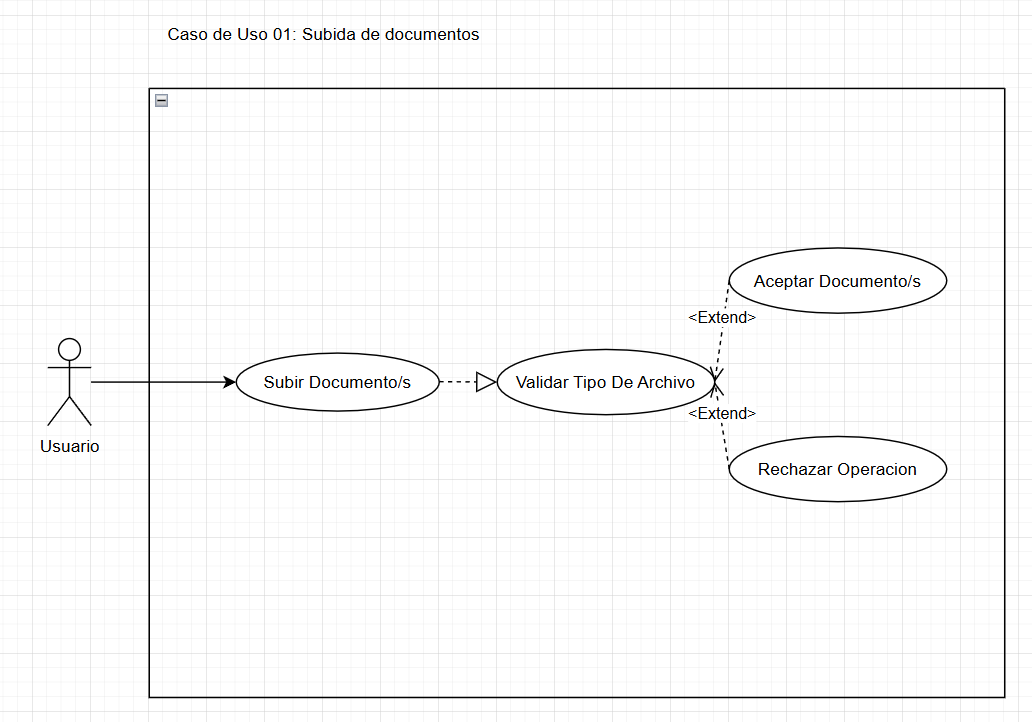
\includegraphics[width=0.75\linewidth]{images/CU-01.png}
    \caption{CU-01}
    \label{fig:CU-01}
\end{figure}

\paragraph{Explicación conceptual:}
Al subir un documento, el sistema debe validar que el tipo de archivo sea compatible: no se aceptan documentos de audio (como archivos MP4) ni imágenes (jpg, png, etc.). Los PDF con texto no seleccionable (equivalentes a imágenes) son aceptados técnicamente, pero no se garantiza el éxito del procesamiento; la aplicación de OCR fue considerada y se realizaron pruebas preliminares, aunque se trata de una mejora futura, ya que su uso limitaría la calidad del \textit{chunking} dinámico.
Este es un control básico de entrada; en esta misma fase se realizan además el resto de comprobaciones necesarias (tamaño, etc.).

\subsection {CU-02 Preprocesamiento Y Segmentación}

\begin{table}[H]
\centering
\renewcommand{\arraystretch}{1.3} % más espacio entre filas
\begin{tabularx}{\textwidth}{|l|X|}
\hline
\textbf{Identificador} & CU-02 \\
\hline
\textbf{Nombre} & Preprocesamiento Y Segmentación \\
\hline
\textbf{Objetivo} & Obtener únicamente información relevante en el texto, hacer una separación óptima y crear embeddings. \\
\hline
\textbf{Actores} & Principal: Chunk Extractor \newline Secundarios: Ninguno \\
\hline
\textbf{Precondiciones} & Debe haberse ejecutado el CU-01, y depende del flujo, el CU-03 (Se entra en detalle en la explicación), pues para el procesado hacen falta documentos. \\
\hline
\textbf{Disparador (Trigger)} & CU-01 \\
\hline
\textbf{Flujo principal} &
1. CU-01 Correcto. \newline
2. Procesamiento de documentos Indexables. \newline
3. Obtención de embeddings. \\
\hline
\textbf{Flujos alternativos} & Procesamiento de documentos no indexables (OCR) (Futuro). \newline Obtención de embeddings. \\
\hline
\textbf{Excepciones} & Los errores de este caso deberían haber sido prevenidos en el CU-01. \\
\hline
\textbf{Postcondiciones} & Al finalizar este CU obtenemos los embeddings con los que trabajaremos. \\
\hline
\textbf{Entradas} & Los documentos que recibe del CU-01. \\
\hline
\textbf{Salidas} & En este caso concreto, los embeddings no se almacenan de manera persistente, por lo que no se mantienen post-ejecución. \\
\hline
\textbf{Prioridad / Frecuencia} & Alta. \\
\hline
\textbf{Dependencias} & CU-01. \\
\hline
\end{tabularx}
\caption{Ficha del caso de uso CU-02.}
\label{tab:CU-02}
\end{table}

\begin{figure}[H]
    \centering
    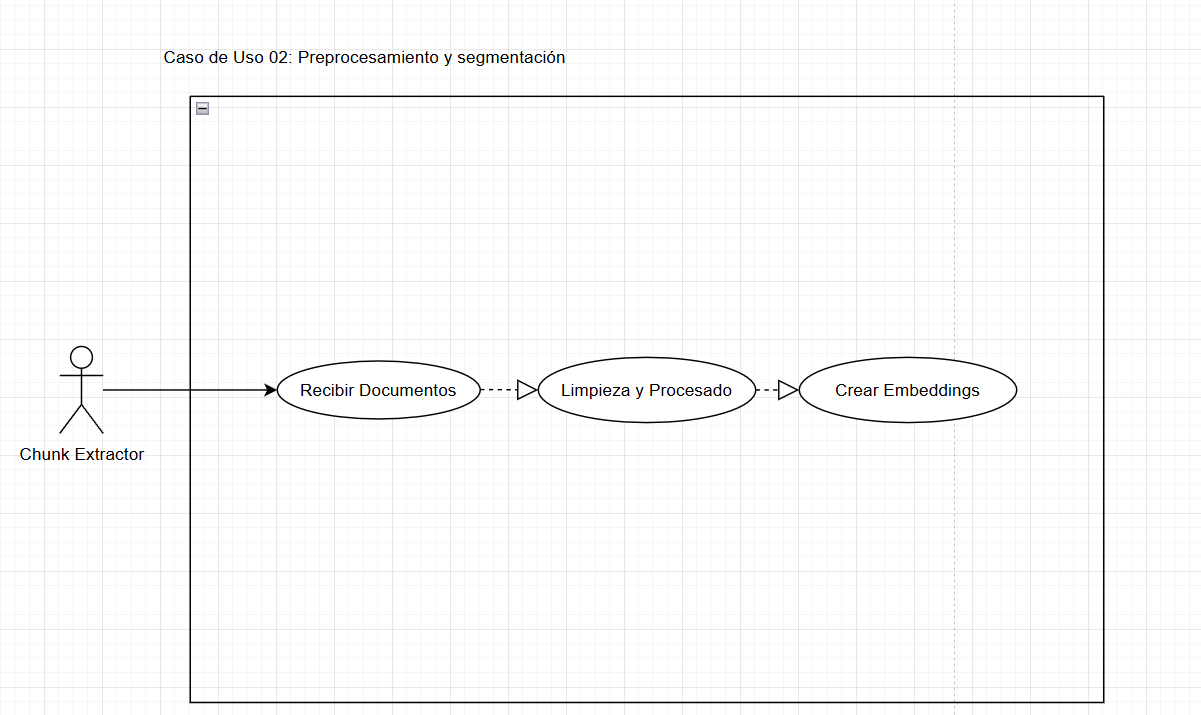
\includegraphics[width=0.75\linewidth]{images/CU-02.png}
    \caption{CU-02}
    \label{fig:CU-02}
\end{figure}

\paragraph{Explicación conceptual:}
Al recibir el documento, el sistema realiza la limpieza y el preprocesado necesarios para su posterior transformación en \textit{embeddings}. Si bien actualmente los \textit{embeddings} no se emplean como mecanismo de persistencia, representan una mejora futura clave al integrar bases de datos vectoriales.

La lógica de extracción se implementa en el módulo (\texttt{chunk\_extractor.py}), orientado a preservar la estructura jerárquica del documento —aspecto fundamental para GraphRAG— mediante los siguientes procesos:

\begin{enumerate}
    \item \textbf{Intento de extracción de hipervínculos:}

    Esta función (\texttt{extract\_links\_with\_detailed\_debug(pdf\_path)}) se encarga de:
    \begin{itemize}
        \item \textbf{Identificar enlaces internos:} Utiliza la librería \texttt{PyMuPDF} para detectar anotaciones de tipo \textit{link} que apunten a páginas dentro del mismo documento.
        \item \textbf{Filtrado por márgenes:} Mediante la función \texttt{get\_page\_margins}, ignora cualquier enlace fuera del área central (10\% de margen), descartando encabezados y pies de página.
        \item \textbf{Recuperación de respaldo (Fallback):} Si el PDF no posee hipervínculos activos, aplica una búsqueda mediante expresiones regulares (\texttt{index\_pattern}) en las primeras 6 páginas para detectar un índice textual basado en numeración y puntos suspensivos.
    \end{itemize}

    \item \textbf{Organización jerárquica del índice:}

    Esta función (\texttt{organizar\_indice(hyperlinks\_data)}) es crítica para la posterior construcción del grafo en NetworkX. Se encarga de:
    \begin{itemize}
        \item \textbf{Detección de niveles:} Analiza la estructura numérica (ej. ``1.2.1'') mediante \texttt{extract\_\allowbreak number\_struc\-ture} para determinar la profundidad de cada sección.
        \item \textbf{Inferencia por indentación:} En ausencia de numeración clara, utiliza la coordenada horizontal ($X$) del enlace para identificar subsecciones (una mayor $X$ implica un nivel de jerarquía inferior).
        \item \textbf{Asignación de parentesco:} Establece relaciones ``Padre-Hijo'' comparando los prefijos numéricos o retrocediendo en la lista de elementos para encontrar el ancestro común más cercano.
    \end{itemize}

    \item \textbf{Extracción estricta de texto entre secciones:}
    Esta función (\texttt{extract\_text\_be\-tween\_sec\-tions\_strict(pdf\_path, links\_data)}) se encarga de:
    \begin{itemize}
        \item \textbf{Localización visual:} No se limita a copiar el texto de la página; utiliza \texttt{find\_title\_\allowbreak in\_page} con algoritmos de lógica difusa (\textit{fuzzy matching}) y comprobación de estilo (negritas) para hallar el punto exacto donde comienza y termina cada sección.
        \item \textbf{Segmentación precisa:} Define el \textit{chunk} desde el final del título de la sección actual hasta el inicio del título de la siguiente sección, permitiendo que un mismo apartado abarque múltiples páginas.
        \item \textbf{Normalización:} Excluye metadatos irrelevantes y limpia el ruido visual del texto extraído.
    \end{itemize}

    \item \textbf{Persistencia de segmentos:}

    Esta función (\texttt{save\_chunks\_to\_file(chunks, output\_file)}) se encarga de:
    \begin{itemize}
        \item \textbf{Serialización:} Almacena los fragmentos procesados en un archivo de salida, incluyendo metadatos clave: ID de sección, título normalizado, nivel jerárquico y referencia al padre.
        \item \textbf{Formateo:} Estructura el contenido de forma legible para facilitar la depuración de las fases posteriores del \textit{pipeline} de RAG.
    \end{itemize}
\end{enumerate}

\subsection {CU-03 Análisis de la pregunta y decisión del agente}

\begin{table}[H]
\centering
\renewcommand{\arraystretch}{1.3} % más espacio entre filas
\begin{tabularx}{\textwidth}{|l|X|}
\hline
\textbf{Identificador} & CU-03 \\
\hline
\textbf{Nombre} & Análisis de la pregunta y decisión del agente. \\
\hline
\textbf{Objetivo} & Según la pregunta, decidir si se utilizan fragmentos parciales del documento (\textit{chunks}) y optimizar la consulta para una recuperación mediante GraphRAG más precisa. \\
\hline
\textbf{Actores} & Principal: Usuario \newline Secundarios: Agente de decisión. \\
\hline
\textbf{Precondiciones} & Deben haberse completado el CU-01 y el CU-02 para disponer de los \textit{embeddings}. \\
\hline
\textbf{Disparador (Trigger)} & Fin del CU-02. \\
\hline
\textbf{Flujo principal} &
1. El usuario hace una pregunta. \newline
2. El agente la recibe. \newline
3. Se decide si se responde con documentos completos o con las secciones de contenido. \newline
4. Si es por secciones el Agente proporciona una pregunta Optimizada para la búsqueda. \\
\hline
\textbf{Flujos alternativos} & En caso de ser el documento completo no se ejecuta el caso 4 del flujo principal. \\
\hline
\textbf{Excepciones} & Los errores posibles deberían haber sido manejados en CU-01. \\
\hline
\textbf{Postcondiciones} & Al finalizar se dispone de la decisión sobre el tipo de respuesta y, en caso de seleccionarse la ruta por secciones, de la consulta optimizada. \\
\hline
\textbf{Entradas} & Pregunta. \\
\hline
\textbf{Salidas} & Tipo de respuesta, pregunta optimizada. \\
\hline
\textbf{Prioridad / Frecuencia} & Alta. \\
\hline
\textbf{Dependencias} & Incluye: CU-01, CU-02. \\
\hline
\end{tabularx}
\caption{Ficha del caso de uso CU-03.}
\label{tab:CU-03}
\end{table}

\begin{figure}[H]
    \centering
    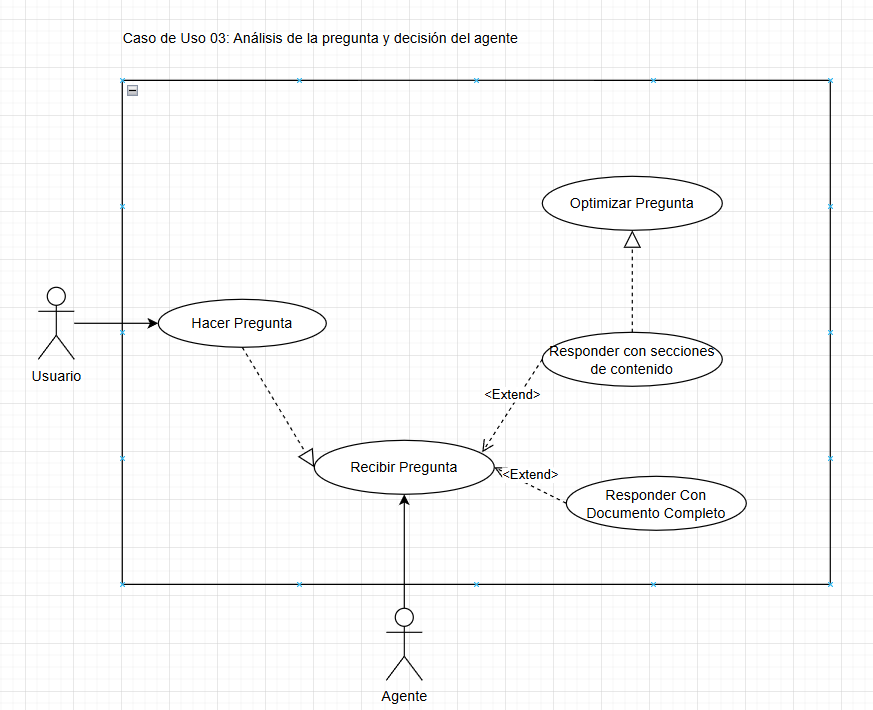
\includegraphics[width=0.75\linewidth]{images/CU-03.png}
    \caption{CU-03}
    \label{fig:CU-03}
\end{figure}

\paragraph{Lógica del Agente de Selección de Estrategia:}
Para optimizar el consumo de recursos y la precisión de las respuestas, se ha implementado un agente inteligente (\texttt{DocumentStrategyAgent}) que actúa como capa intermedia entre la consulta del usuario y el motor de recuperación. Su función principal es determinar si la consulta requiere una búsqueda local (RAG) o una comprensión global del documento.

Este proceso, integrado en la clase \texttt{SmartDocumentProcessor}, sigue la siguiente lógica:

\begin{enumerate}
    \item \textbf{Análisis Dinámico de la Consulta:}
    La función (\texttt{analyze\_query}) envía la pregunta del usuario junto con metadatos del documento (número de páginas, tipo de archivo) a un modelo de lenguaje (LLM). El agente evalúa dos escenarios:
    \begin{itemize}
        \item \textbf{Acceso Parcial (RAG):} Se activa si la consulta busca datos específicos, hechos puntuales o secciones concretas (ej. ``¿Cuál es el presupuesto en la sección 3?'').
        \item \textbf{Acceso Total (Full Document):} Se activa si la consulta requiere entender el documento como un todo, realizar resúmenes globales o encontrar inconsistencias transversales.
    \end{itemize}

    \item \textbf{Clasificación y Razonamiento:}
    El agente no solo devuelve una decisión, sino que mediante la función (\texttt{\_parse\_decision}) extrae:
    \begin{itemize}
        \item \textbf{Estrategia:} \textit{Partial} o \textit{Full}.
        \item \textbf{Nivel de Confianza:} Un valor numérico que permite auditar la fiabilidad de la elección.
        \item \textbf{Razonamiento:} Una explicación textual de por qué se eligió dicha ruta, mejorando la interpretabilidad del sistema.
    \end{itemize}

    \item \textbf{Ejecución de Rutas de Respuesta:}
    Dependiendo de la decisión y del modo de operación seleccionado, el procesador (\texttt{process\_query}) ejecuta:
    \begin{itemize}
        \item \textbf{Modo RAG Individual/Consolidado:} Utiliza el sistema de grafos (\texttt{NetworkX}) para recuperar subsecciones relevantes de uno o varios documentos.
        \item \textbf{Modo de Contexto Extendido:} En caso de elegir la estrategia \textit{Full}, se invoca la función \texttt{\_process\_full\_documents}, que reconstruye el documento manteniendo el orden jerárquico de secciones y lo inyecta en una ventana de contexto ampliada (hasta 60.000 tokens).
    \end{itemize}

    \item \textbf{Interfaz Interactiva y Control de Flujo:}
    A través de (\texttt{interactive\_chat}), el sistema permite al usuario alternar entre modos de respuesta (Individual vs. Consolidada) y activar la visualización de los grafos generados, permitiendo una depuración en tiempo real del proceso de recuperación.
\end{enumerate}

\subsection {CU-04 Generación de Respuesta}

\begin{table}[H]
\centering
\renewcommand{\arraystretch}{1.3} % más espacio entre filas
\begin{tabularx}{\textwidth}{|l|X|}
\hline
\textbf{Identificador} & CU-04 \\
\hline
\textbf{Nombre} & Generación de Respuesta \\
\hline
\textbf{Objetivo} & Secuencia de Generación de la Respuesta. \\
\hline
\textbf{Actores} & Principal: Usuario \newline Secundarios: LLM \\
\hline
\textbf{Precondiciones} & Debemos haber completado el CU-03. \\
\hline
\textbf{Disparador (Trigger)} & Fin del CU-03. \\
\hline
\textbf{Flujo principal} &
1. El usuario selecciona el tipo de respuesta. \newline
2. Se ejecuta el proceso según la respuesta. \newline
3. El modelo Genera la respuesta. \\
\hline
\textbf{Flujos alternativos} & 1-Eran necesarios los documentos completos y exceden la ventana de contexto del modelo en uso. \newline 2-Se cortará el excedente. \\
\hline
\textbf{Excepciones} & Si se corta el excedente la respuesta puede ser poco indicativa de la realidad. \\
\hline
\textbf{Postcondiciones} & El usuario recibe la respuesta según formato solicitado. \\
\hline
\textbf{Entradas} & Lo obtenido en los otros CU. \\
\hline
\textbf{Salidas} & Respuesta en formato texto. \\
\hline
\textbf{Prioridad / Frecuencia} & Alta. \\
\hline
\textbf{Dependencias} & Incluye: CU-01, CU-02, CU-03. \\
\hline
\end{tabularx}
\caption{Ficha del caso de uso CU-04.}
\label{tab:CU-04}
\end{table}

\begin{figure}[H]
    \centering
    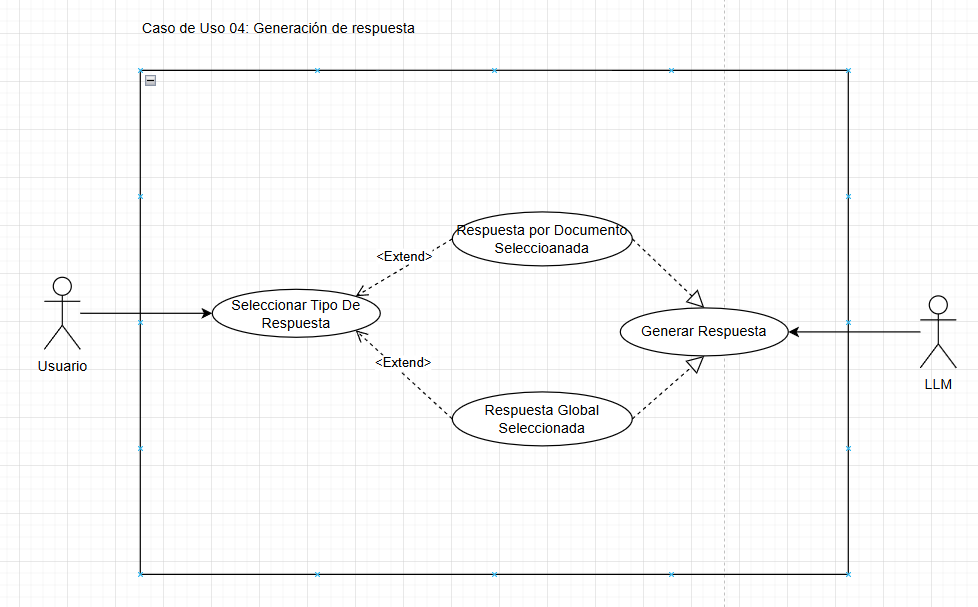
\includegraphics[width=0.75\linewidth]{images/CU-04.png}
    \caption{CU-04}
    \label{fig:CU-04}
\end{figure}
\newpage

\paragraph{Casos de Uso e Interacción (CU-04):}
La lógica de interacción se centraliza en el método \texttt{inter\-active\_chat}, el cual materializa el caso de uso \textbf{CU-04: Seleccionar Tipo de Respuesta}. Como se observa en el diagrama de la Figura 5.4, el usuario interactúa con el sistema para decidir cómo se procesará la información recuperada por el LLM.

Este componente gestiona la ejecución mediante los siguientes estados y opciones:

\begin{enumerate}
    \item \textbf{Modo 1: Respuestas Individuales (Default):}
    Corresponde a la extensión \textit{<<Extend>> Respuesta por Documento Seleccionada}. El sistema genera una respuesta independiente por cada archivo PDF cargado, utilizando grafos de conocimiento locales. Es ideal para comparar normativas o pliegos técnicos de distintos proveedores de forma aislada.

    \item \textbf{Modo 2: Respuesta Consolidada:}
    Activa la extensión \textit{<<Extend>> Respuesta Global Seleccionada}. Mediante la función \texttt{generate\_consolidated\_graph\_response}, el sistema realiza un análisis transversal de todos los documentos, unificando los grafos de NetworkX para ofrecer una visión de conjunto.

    \item \textbf{Gestión de Observabilidad (Visualización):}
    El sistema permite activar la visualización de grafos en tiempo real (\texttt{visualize\_graphs = True}). Esta funcionalidad genera representaciones gráficas (PNG) de las relaciones de conocimiento detectadas, lo que permite al usuario (o desarrollador) validar la calidad de la recuperación semántica.

    \item \textbf{Ciclo de Control:}
    La implementación utiliza un bucle persistente que permite cambiar la estrategia de consulta (\texttt{modo 1/2}) y las opciones de depuración sin necesidad de reiniciar el sistema ni volver a procesar los documentos, optimizando así el tiempo de respuesta en sesiones de análisis extensas.
\end{enumerate}

El flujo finaliza con la intervención del actor \textbf{LLM}, que recibe el contexto estructurado según el modo seleccionado para generar la respuesta final al usuario.

\newpage
\section{Diagramas de comportamiento}
\begin{figure}[htb!]
    \centering
    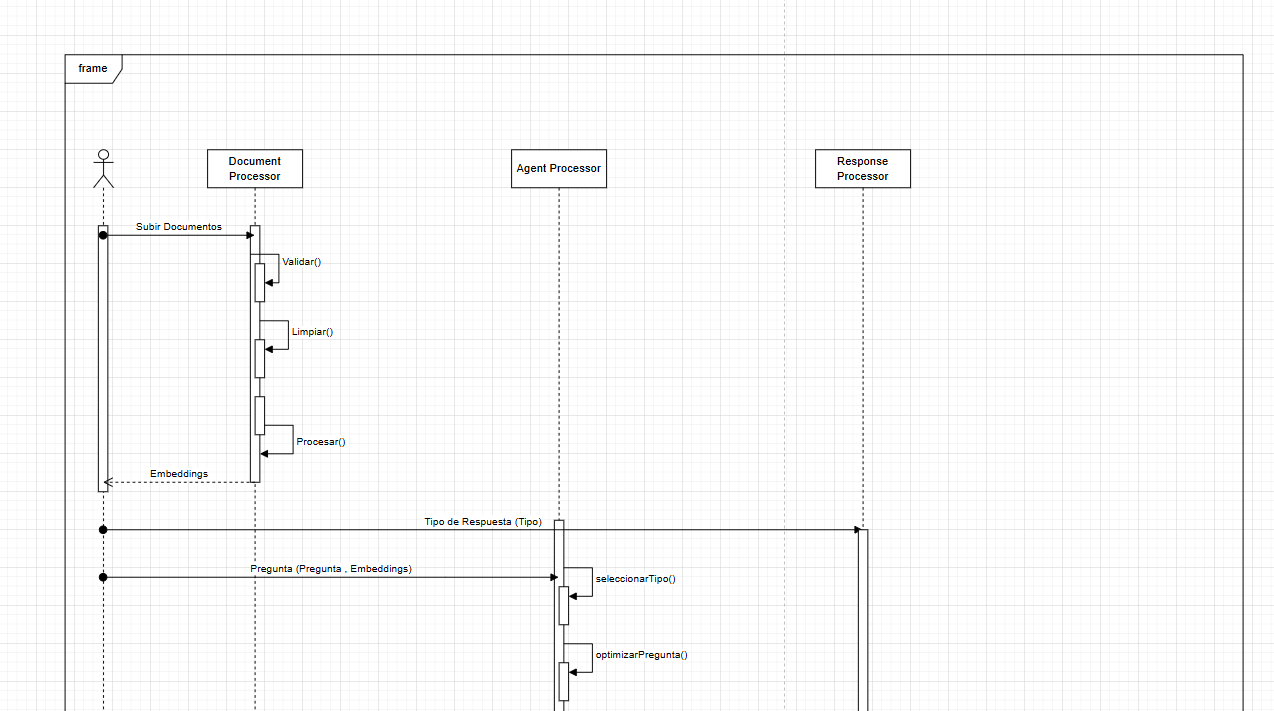
\includegraphics[width=1\linewidth]{images/Seq-01.png}
    \label{fig:seq01}
\end{figure}

\begin{figure}[htb!]
    \centering
    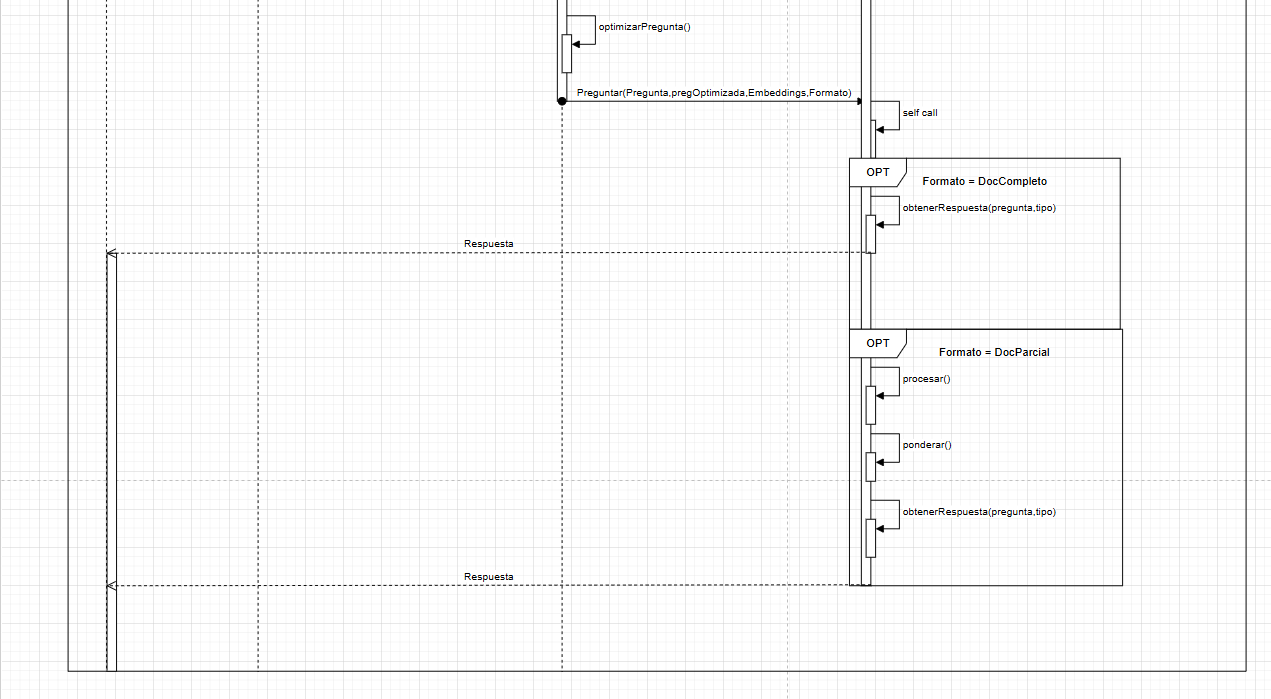
\includegraphics[width=1\linewidth]{images/Seq-02.png}
    \caption{Diagrama de Secuencia}
    \label{fig:seq02}
\end{figure}

\newpage

\paragraph{Pipeline de Procesamiento y Resolución de Consultas:}
En este diagrama de secuencia se muestra cómo sería el flujo (uno de los posibles) dentro del sistema.
El comportamiento dinámico del sistema se articula a través de una arquitectura de pipeline dividida en tres fases fundamentales, coordinando la preparación de la base de conocimiento con la ejecución de agentes inteligentes para la generación de respuestas.

\begin{enumerate}
    \item \textbf{Fase de Ingestión y Estructuración (\textit{Document Processor}):}
    En esta etapa, el sistema transforma documentos PDF no estructurados en una red de conocimiento jerárquica:
    \begin{itemize}
        \item \textbf{Validación y Normalización:} Se realiza una limpieza profunda del texto para eliminar ruido visual y asegurar la integridad de los datos procesados.
        \item \textbf{Segmentación Jerárquica:} Utilizando la lógica de \texttt{chunk\_extractor.py}, el sistema identifica secciones y subsecciones, preservando las relaciones de dependencia originales del documento.
        \item \textbf{Indexación Vectorial:} Se generan \textit{embeddings} para cada segmento, permitiendo búsquedas semánticas eficientes en fases posteriores.
    \end{itemize}

    \item \textbf{Fase de Orquestación y Decisión (\textit{Agent Processor}):}
    Una vez consolidada la base de datos, el sistema actúa como un agente inteligente de decisión:
    \begin{itemize}
        \item \textbf{Análisis de Intención:} El \texttt{DocumentStrategyAgent} evalúa la consulta para determinar si se requiere una búsqueda de datos específicos (RAG) o un análisis global (Contexto Completo).
        \item \textbf{Optimización Semántica:} En la ruta RAG, se ejecuta un proceso de refinamiento de la consulta para extraer términos clave, maximizando la precisión de la recuperación en el grafo.
    \end{itemize}

    \item \textbf{Fase de Recuperación y Generación (\textit{Response Processor}):}
    La fase final integra la información recuperada con el modelo de lenguaje:
    \begin{itemize}
        \item \textbf{Recuperación sobre Grafo (\textit{GraphRAG}):} El sistema no solo busca fragmentos aislados, sino que utiliza \texttt{NetworkX} para realizar una ``Propagación Familiar''. Esto permite incluir secciones ascendentes (padres) y descendentes (hijos) del nodo relevante, con el objetivo de proporcionar al LLM un contexto estructural más completo que el fragmento aislado.
        \item \textbf{Ponderación Híbrida:} Se combinan métricas de similitud de coseno, BM25 y centralidad de grafo (\textit{PageRank}) para seleccionar los fragmentos más informativos.
        \item \textbf{Generación de Respuesta:} El LLM procesa el contexto curado para ofrecer una respuesta que respete la jerarquía del documento, citando explícitamente las secciones de origen.
    \end{itemize}
\end{enumerate}

\begin{figure}
    \centering
    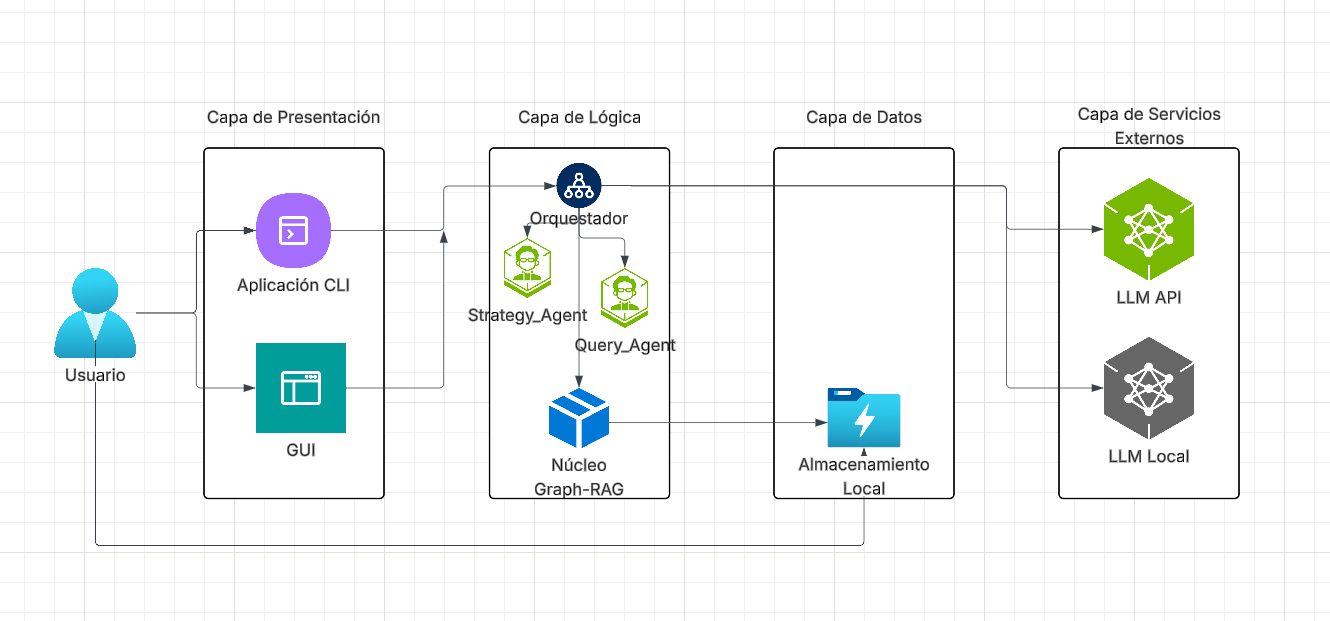
\includegraphics[width=1\linewidth]{images/Diagrama_Arquitectura.png}
    \caption{Diagrama de Arquitectura}
    \label{fig:Arquiteture_Diagram}
\end{figure}

\begin{figure}
    \centering
    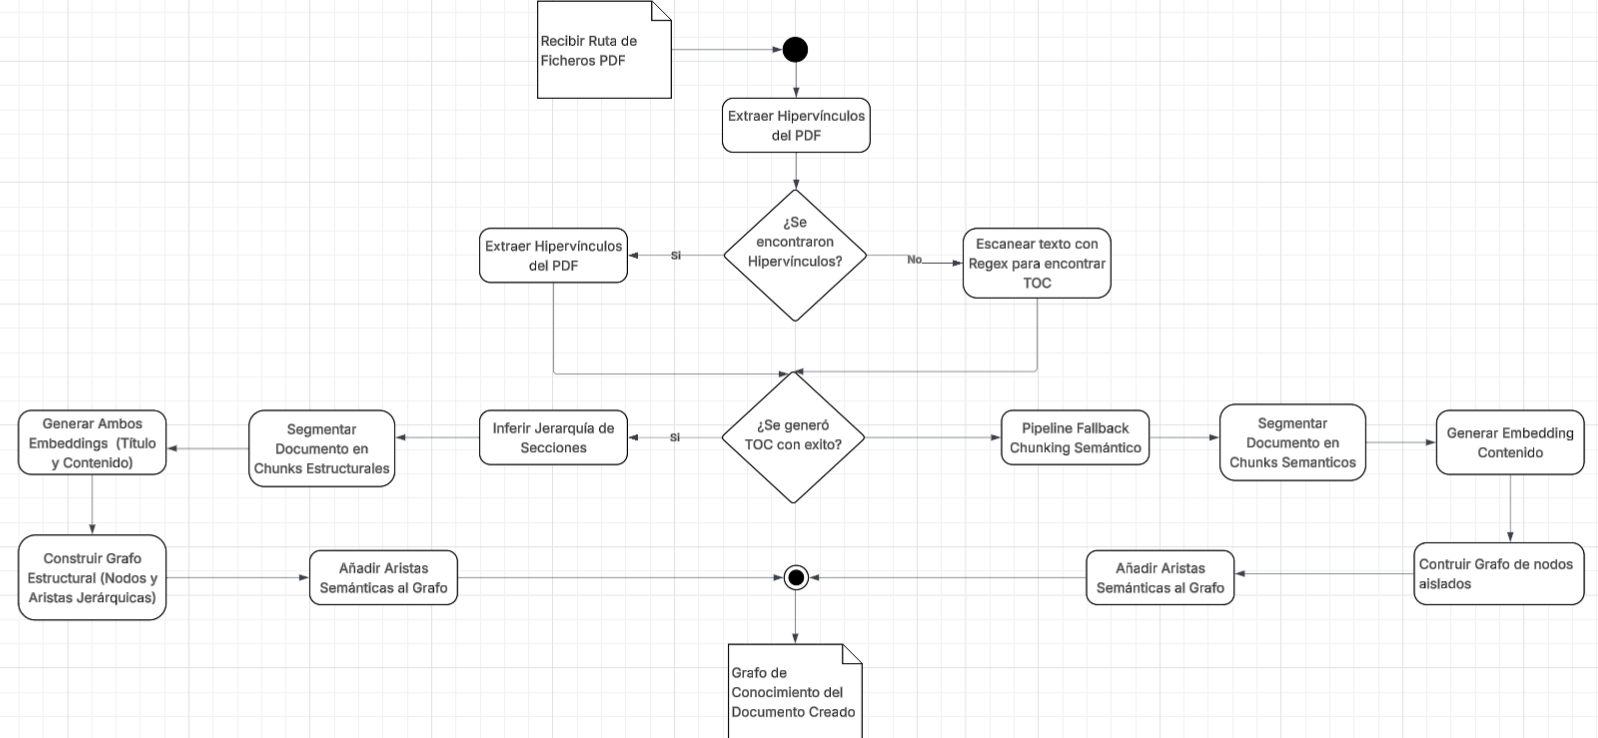
\includegraphics[width=1\linewidth]{images/Diagrama_Actividad_CU-02.png}
    \caption{Especificación diagrama de Actividad CU-02}
    \label{fig:activitydiag01}
\end{figure}

      \chapter{Implementación}\label{cap6}

\newpage
\section{Entorno y Tecnologías}

Para el desarrollo e implementación del sistema, se ha seleccionado un conjunto de tecnologías de código abierto que permiten el procesamiento local de datos, garantizando la privacidad de la información y la soberanía sobre los modelos de inteligencia artificial empleados, ya que, en el caso de una empresa privada, podría preferirse no utilizar modelos externos por razones de privacidad de los datos.

\subsection{Infraestructura de Cómputo y Aceleración}
Dada la carga computacional que requiere la inferencia de modelos de lenguaje y la generación masiva de vectores, se ha hecho uso de la arquitectura de computación paralela de NVIDIA:

\begin{itemize}
    \item \textbf{NVIDIA CUDA (Compute Unified Device Architecture):} Se utiliza como plataforma de computación paralela para permitir que las librerías de \textit{deep learning} (como \texttt{PyTorch}, que sustenta a \texttt{SentenceTransformers}) y el motor \texttt{Ollama} descarguen las operaciones matemáticas pesadas en la GPU. Esto reduce drásticamente el tiempo de generación de \textit{embeddings} y aumenta la velocidad de generación de texto (\textit{tokens per second}) en comparación con el uso exclusivo de la CPU.
\end{itemize}

\subsection{Lenguaje de Programación y Entorno de Ejecución}
La implementación principal se ha realizado en \textbf{Python 3.10+}, aprovechando su maduro ecosistema de librerías para el procesamiento de lenguaje natural (NLP) y estructuras de datos complejas. El entorno de desarrollo se ha gestionado mediante un entorno virtual para asegurar la reproducibilidad de las dependencias.

\subsection{Infraestructura de Modelos de Lenguaje (LLM)}
\begin{itemize}
    \item \textbf{Ollama:} Se utiliza como motor de inferencia local para el despliegue del modelo \texttt{llama3.1:8b}. Esta herramienta permite gestionar el ciclo de vida del modelo y ajustar parámetros críticos como el \texttt{num\_ctx} (ventana de contexto), el cual se ha configurado hasta en 60,000 tokens para el procesamiento de documentos completos.
    \item \textbf{Sentence-Transformers:} Para la generación de \textit{embeddings}, se emplea el modelo \texttt{all-\allowbreak MiniLM-\allowbreak L6-v2}. Este modelo ofrece un equilibrio óptimo entre velocidad de cómputo y calidad en la representación vectorial de fragmentos de texto.
    \item \textbf{Cross-Encoders:} Se ha integrado el modelo \nolinkurl{cross-encoder/ms-marco-MiniLM-L-6-v2} para realizar tareas de \textit{reranking}. A diferencia de los \textit{bi-encoders}, este modelo analiza pares consulta-documento de forma conjunta, mejorando drásticamente la precisión del orden de relevancia final.
\end{itemize}

\subsection{Procesamiento de Documentos y Grafos}
\begin{itemize}
    \item \textbf{PyMuPDF (fitz):} Librería de alto rendimiento utilizada para la manipulación de archivos PDF. Es la pieza clave para extraer metadatos, identificar hipervínculos internos y obtener las coordenadas de los cuadros de texto necesarias para inferir la jerarquía.
    \item \textbf{NetworkX:} Librería especializada en el estudio de redes complejas. Se utiliza para construir el grafo dirigido (\texttt{DiGraph}) donde cada nodo representa una sección del documento y las aristas definen relaciones jerárquicas, secuenciales o semánticas.
    \item \textbf{Rank-BM25:} Implementación del algoritmo de relevancia \textit{Best Matching 25}. Se integra en el sistema de búsqueda híbrida para complementar la búsqueda vectorial con coincidencias exactas de términos clave.
\end{itemize}

\subsection{Otras Librerías de Apoyo}
\begin{itemize}
    \item \textbf{TheFuzz:} Utilizada para el \textit{fuzzy matching} de títulos de secciones, permitiendo que el sistema sea resiliente a pequeñas variaciones de formato o errores de extracción.
    \item \textbf{Tiktoken:} Herramienta de \textit{tokenización} utilizada para contabilizar con precisión el volumen de información enviado al modelo y prevenir el desbordamiento de la ventana de contexto.
    \item \textbf{Matplotlib:} Empleada para la generación de las representaciones visuales de los subgrafos de consulta, facilitando la auditoría del proceso de recuperación.
\end{itemize}

\newpage
\section{Procesamiento de Documentos y Extracción Estricta}
El sistema se ha diseñado bajo una arquitectura modular donde la integridad de la estructura jerárquica del documento es el pilar fundamental. A continuación, se detallan los algoritmos y procesos técnicos que permiten la transformación de documentos PDF en una base de conocimiento funcional para RAG.
La lógica de extracción, implementada en el módulo \texttt{chunk\_extractor.py}, trasciende la simple recuperación de texto plano para enfocarse en la topología del documento.

\subsection{Algoritmo de Extracción y Limpieza}
La función \texttt{extract\_links\_with\_detailed\_debug} actúa como el punto de entrada. Utiliza la librería \texttt{PyMuPDF} para identificar metadatos de navegación. El proceso sigue un flujo de decisión:
\begin{itemize}
    \item \textbf{Detección de Hipervínculos:} Se utiliza \texttt{page.get\_links()} para extraer anotaciones de salto interno. Se recupera el texto contenido en el rectángulo del enlace (\texttt{textbox}) y se vincula a su página de destino (\texttt{target\_page}).
    \item \textbf{Filtro de Márgenes:} Mediante \texttt{get\_page\_margins}, se define un área de interés que excluye el 10\% de cada borde de la página. El objetivo es reducir elementos de ruido como números de página, encabezados y pies de página que podrían contaminar la calidad de los \textit{embeddings}.
\end{itemize}

A continuación se ilustra gráficamente el filtro de márgenes. En los tipos de archivo para los que se ha especializado el sistema, es habitual encontrar texto repetido, títulos de sección, firmas digitales u otros contenidos en las zonas superior, inferior o lateral de la página; por ejemplo:

\begin{figure}[H]
    \centering
    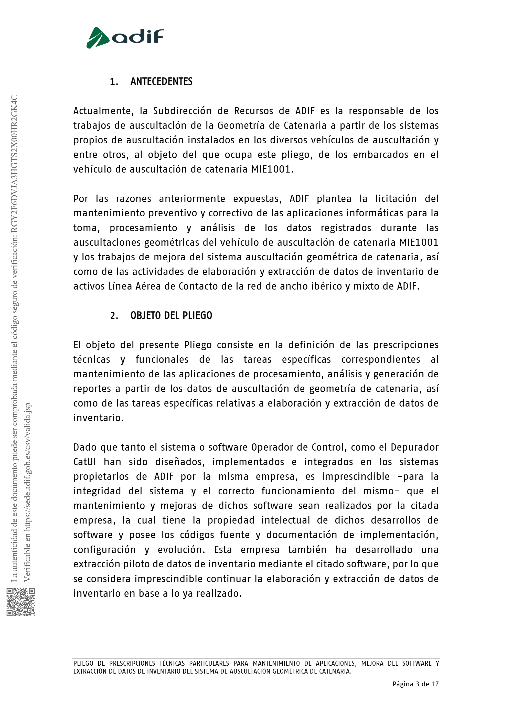
\includegraphics[width=0.8\textwidth]{images/PliegoSinMargenes.png}
    \caption{Página de un pliego técnico de ADIF como ejemplo de contenido en márgenes}
    \label{fig:PliegoConBordes}
\end{figure}

Como se aprecia en la imagen, existe texto tanto en el margen izquierdo como en el superior. Aunque individualmente puede parecer escaso, en documentos de cientos de páginas representa una cantidad considerable de contenido irrelevante; tras aplicar el filtro, el área efectiva queda reducida a lo siguiente:

\begin{figure}[H]
    \centering
    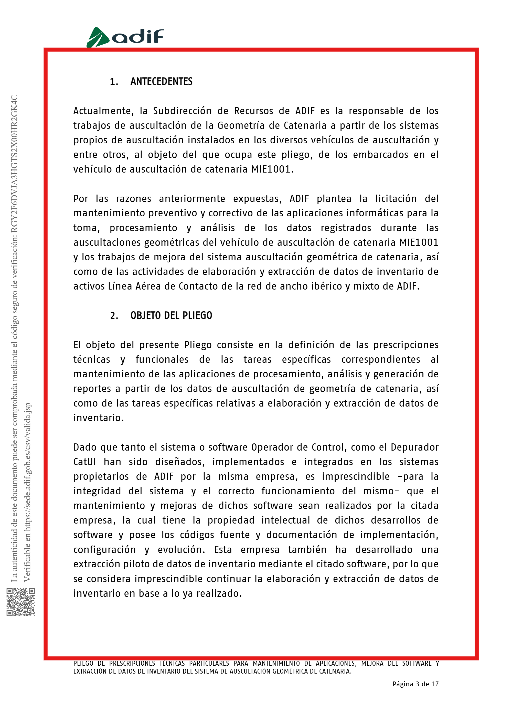
\includegraphics[width=0.8\textwidth]{images/PliegoMargenesQuitados.png}
    \caption{La parte dentro del rectángulo rojo representa lo que se verá}
    \label{fig:PliegoMargenes}
\end{figure}

\newpage

\subsection{Reconstrucción Jerárquica mediante Posición X}
En la función \texttt{organizar\_indice}, se implementa una lógica de inferencia para documentos que carecen de una numeración explícita (ej. 1.1, 1.2). El sistema utiliza la propiedad \texttt{X} (posición horizontal) de la coordenada de origen del enlace:
\begin{itemize}
    \item \textbf{Indentación:} Si un elemento presenta una coordenada \texttt{X} significativamente mayor que el anterior, se clasifica automáticamente como una subsección (\textit{hijo}).
    \item \textbf{Parentesco:} El sistema asigna un ID jerárquico y vincula el nodo a su padre más cercano en la pila de procesamiento, permitiendo reconstruir el árbol documental completo.
\end{itemize}

\newpage
\section{Arquitectura del Grafo de Conocimiento (NetworkX)}

Tras la fase de segmentación y extracción, los fragmentos de información (\textit{chunks}) no se almacenan como elementos aislados, sino que se integran en una estructura de grafo dirigido ($\texttt{DiGraph}$) utilizando la librería \texttt{NetworkX}. Esta arquitectura es la que habilita la capacidad de \textbf{GraphRAG}, permitiendo realizar búsquedas que respetan tanto la jerarquía como la semántica del documento original.

\subsection{Modelado de Nodos y Atributos}
Cada nodo en el grafo representa una unidad de información (sección o subsección). Para garantizar la trazabilidad y la eficacia en la recuperación, a cada nodo se le asignan los siguientes atributos técnicos:
\begin{itemize}
    \item \textbf{Content:} El cuerpo de texto normalizado y limpio.
    \item \textbf{Level:} Profundidad jerárquica (ej. Nivel 0 para capítulos, Nivel 1 para secciones).
    \item \textbf{Page Range:} Tupla con la página de inicio y fin para permitir la citación precisa en la respuesta final.
    \item \textbf{Vector Embedding:} Representación numérica del contenido generada mediante el modelo \texttt{all-\allowbreak MiniLM-\allowbreak L6-v2}.
\end{itemize}

\subsection{Tipología de Aristas y Relaciones Multimodales}
La innovación del sistema reside en la coexistencia de diferentes tipos de aristas, lo que permite navegar el documento de forma no lineal:
\begin{itemize}
    \item \textbf{Aristas Jerárquicas:} Definen la relación \textit{Padre-Hijo}. Se crean automáticamente basándose en el ID de la sección y la indentación detectada en el PDF.
    \item \textbf{Aristas Secuenciales:} Conectan fragmentos adyacentes dentro del flujo de lectura original, permitiendo al sistema recuperar el contexto inmediato (anterior y posterior) de un dato específico.
    \item \textbf{Aristas Semánticas:} Implementadas mediante el método \texttt{add\_semantic\_edges}. Se calculan relaciones de similitud de coseno entre todos los nodos del grafo; si la similitud supera un umbral de $0.65$, se establece un vínculo bidireccional. Esto permite conectar conceptos relacionados que se encuentran en capítulos distantes del documento.
\end{itemize}

\subsection{Algoritmo de Propagación de Relevancia (Family Scores)}
Para mitigar el problema de los fragmentos con poco texto que carecen de peso semántico por sí mismos, se ha implementado la técnica de \textbf{Propagación Familiar}. El sistema ajusta la relevancia de un nodo en función de su entorno:

\begin{equation}
Score_{final}(n) = (Score_{similitud}(n) \times w_{1}) + (\max(Score_{familia}(n)) \times w_{2})
\end{equation}

Donde $w_{1}$ y $w_{2}$ son pesos configurables (con un valor de $0{,}5$ en la configuración empleada). Esta lógica favorece que, si una sección secundaria es relevante, su sección ``padre'' (que contiene el contexto general) también sea recuperada para su inclusión en el \textit{prompt} del modelo.

\begin{figure}[h]
    \centering
    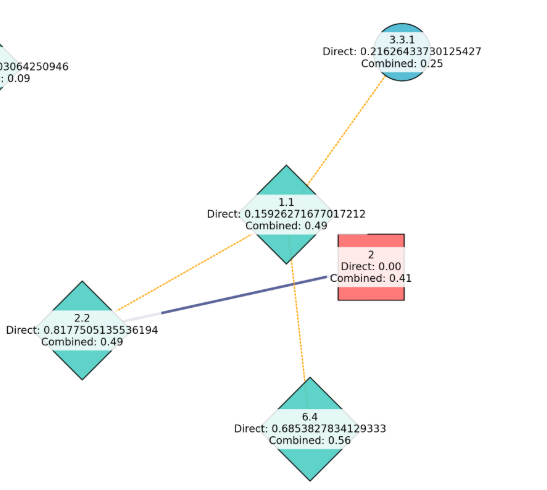
\includegraphics[width=0.8\textwidth]{images/ConexionSemantico_Jerarquico.png}
    \caption{Gráfico con un nodo central conectado mediante similitud familiar (azul) y semántica (amarilla)}
    \label{fig:ConexionSemantico_Jerarquico}
\end{figure}

\newpage
\subsection{Recuperación de Contexto mediante Centralidad}
Finalmente, el sistema utiliza algoritmos de centralidad de grafos para seleccionar la información más densa en contenido. Al realizar una consulta, el sistema extrae un subgrafo de interés y aplica \textbf{PageRank} para identificar qué nodos actúan como ejes centrales de información dentro de la selección. La función \texttt{get\_optimal\_context} filtra y ordena estos nodos, limitando la cantidad de texto enviado al LLM para no saturar su ventana de contexto y favoreciendo una mayor representatividad del documento dentro del presupuesto de tokens disponible.

\begin{figure}[h]
    \centering
    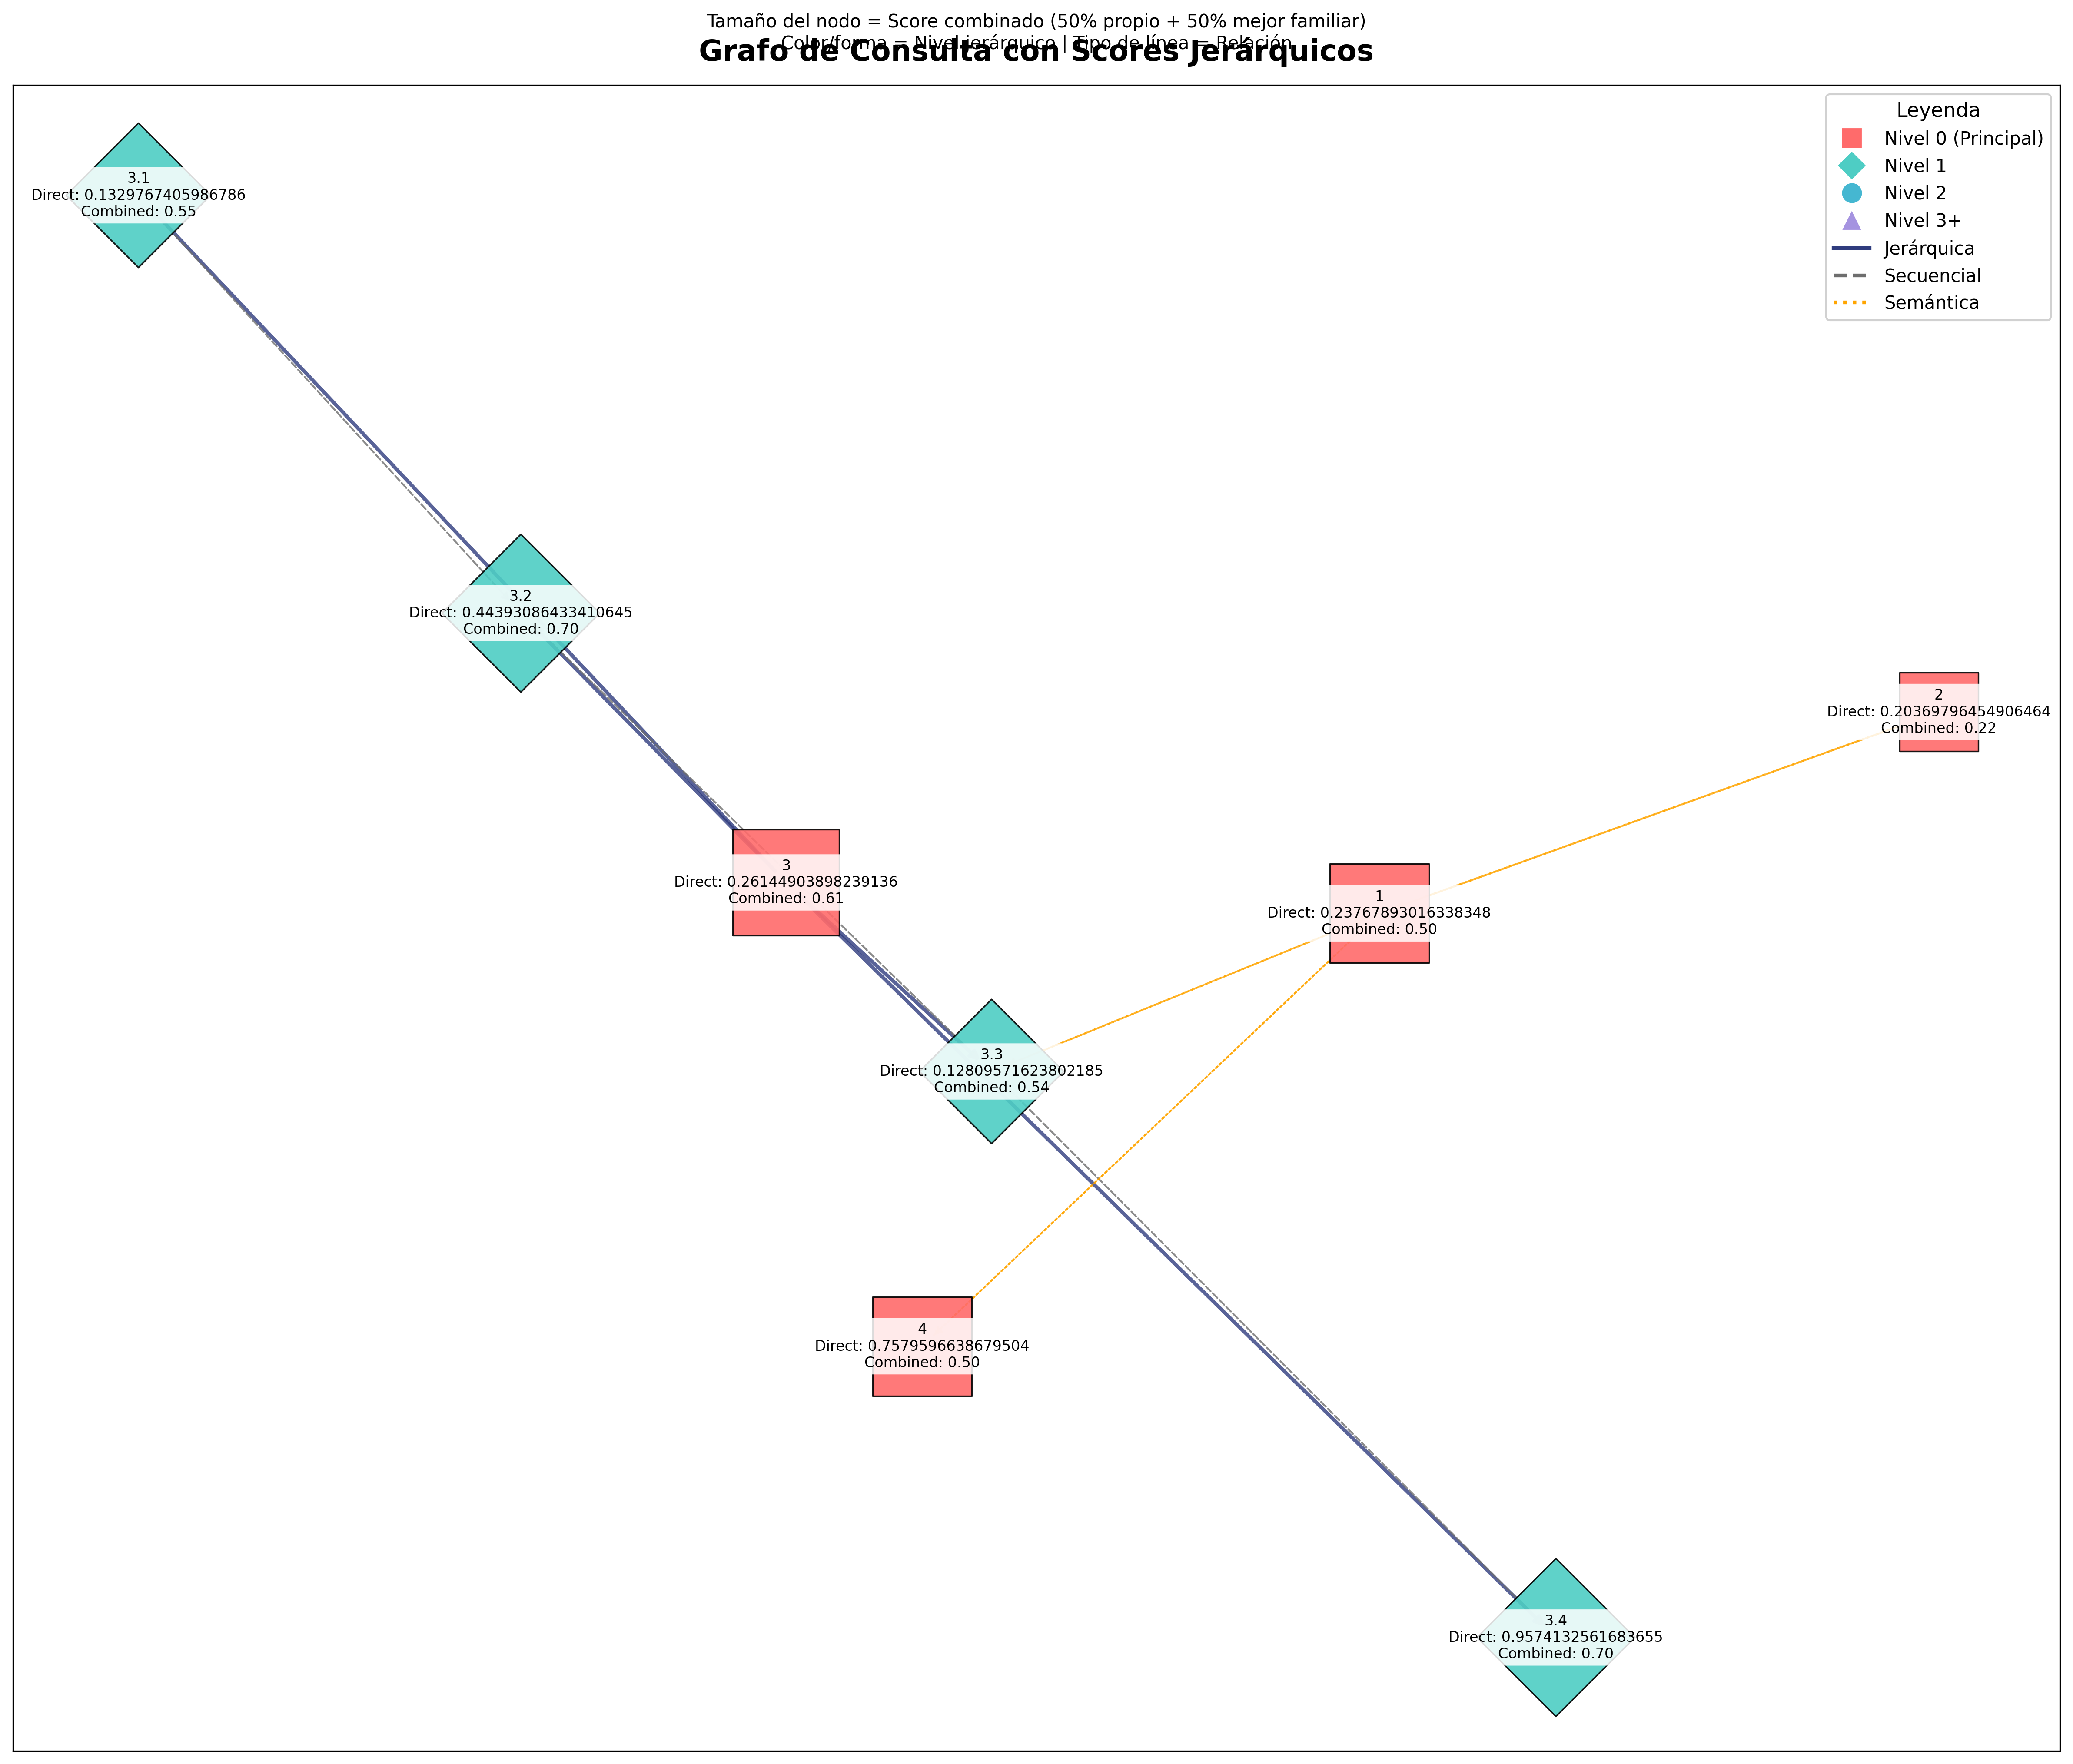
\includegraphics[width=1\textwidth]{images/graficoQuery.png}
    \caption{Ejemplo de gráfico generado}
    \label{fig:GraficoGenerado}
\end{figure}

\newpage
\section{Pipeline de Búsqueda Híbrida y Reranking}

Para maximizar la precisión en la recuperación de información, el sistema implementa un flujo de trabajo multietapa que combina algoritmos de búsqueda léxica y semántica, culminando en un proceso de re-clasificación profunda (\textit{reranking}). Este enfoque mitiga las limitaciones individuales de cada técnica, como el ruido semántico o la incapacidad de capturar sinónimos.

\subsection{Estrategia de Búsqueda Híbrida (BM25 + Embeddings)}
La función \texttt{query\_chunks\_hybrid} coordina la recuperación inicial utilizando dos motores paralelos:
\begin{itemize}
    \item \textbf{Recuperación Léxica (BM25):} Mediante la librería \texttt{Rank-BM25}, el sistema analiza la coincidencia exacta de términos clave. Esto es vital para identificar códigos técnicos, normativas o términos específicos que los modelos de \textit{embeddings} podrían diluir en el espacio vectorial.
    \item \textbf{Recuperación Semántica:} Se utiliza el modelo \texttt{all-\allowbreak MiniLM-\allowbreak L6-v2} para calcular la similitud del coseno entre la consulta y los fragmentos. A diferencia de un RAG estándar, se aplica un proceso de \textbf{sub-chunking semántico} mediante \texttt{RecursiveCharacterTextSplitter}, dividiendo cada sección en micro-fragmentos de 100 caracteres para localizar respuestas precisas dentro de secciones extensas.
\end{itemize}

\subsection{Estrategia de Doble Granularidad: Sub-chunking Semántico}
Una de las innovaciones clave en la implementación del buscador es la superposición de dos niveles de granularidad. Mientras que el grafo gestiona unidades lógicas (secciones), la búsqueda vectorial opera sobre micro-fragmentos generados mediante \texttt{RecursiveCharacterTextSplitter}:
\begin{itemize}
    \item \textbf{Nivel Macro (Grafo):} Proporciona el contexto estructural y las relaciones de parentesco.
    \item \textbf{Nivel Micro (Sub-chunks):} Se generan fragmentos de 100 caracteres con un solapamiento (\textit{overlap}) de 20 caracteres. Esto permite que el modelo de \textit{embeddings} capture la semántica exacta de una frase técnica sin la "dilución" que ocurre cuando se vectorizan párrafos muy extensos.
\end{itemize}
Esta aproximación permite que, ante una consulta específica, el sistema localice el sub-chunk exacto y, gracias a la estructura de grafo, recupere automáticamente la sección completa a la que pertenece.

\subsection{Ponderación de Resultados y Fusión}
Los resultados de ambos motores se normalizan y combinan. El sistema otorga un peso del $67,5\%$ a la similitud semántica y un $32,5\%$ a la puntuación BM25. Esta ponderación busca que la respuesta tenga sentido conceptual sin sacrificar la precisión en la recuperación de términos clave utilizados por el usuario.

\subsubsection{Justificación de Umbrales y Ponderaciones}
Los valores de configuración se han ajustado tras una fase de pruebas empíricas:
\begin{itemize}
    \item \textbf{Umbral Semántico ($\tau = 0.65$):} Se seleccionó para evitar el fenómeno de ``grafo denso'', donde demasiadas conexiones semánticas irrelevantes difuminan la estructura jerárquica.
    \item \textbf{Ponderación Híbrida (67.5\% Vectorial / 32.5\% BM25):} Este equilibrio favorece la comprensión de conceptos sobre la coincidencia de palabras, pero mantiene la capacidad de encontrar términos técnicos específicos (códigos de error, nombres de funciones) que el motor léxico detecta con mayor fiabilidad.
\end{itemize}

\subsection{Re-clasificación Profunda mediante Cross-Encoder}
Debido a que los modelos de \textit{bi-encoders} (usados para los \textit{embeddings}) procesan la consulta y el documento de forma independiente, pueden perder matices relacionales. Para resolver esto, se implementa una etapa de \textbf{Reranking} con el modelo \nolinkurl{cross-encoder/ms-marco-MiniLM-L-6-v2}:
\begin{itemize}
    \item El sistema toma los mejores candidatos de la búsqueda híbrida y los somete a una comparación por pares (consulta, fragmento).
    \item El \textit{Cross-Encoder} genera una puntuación de relevancia mucho más precisa, ya que analiza la interacción completa entre las palabras de la pregunta y el contenido del fragmento.
    \item Solo aquellos fragmentos que superan el umbral de confianza tras el re-rankeo (\texttt{min\_similarity}) son considerados para la fase final de generación.
\end{itemize}

\subsection{Integración de Contexto Jerárquico}
Una vez obtenidos los fragmentos finales, el sistema no los entrega al LLM de forma desordenada. Se invoca a \texttt{get\_context\_with\_hierarchy} para reconstruir la estructura documental: los fragmentos se agrupan por documento de origen y se ordenan según su \texttt{section\_id}. Esto permite que el modelo de lenguaje reciba un contexto coherente, respetando el orden lógico del autor original, lo que reduce drásticamente las alucinaciones en la respuesta final.

\newpage
\section{Orquestación y Agentes Inteligentes}

El sistema no se limita a una recuperación estática de datos, sino que implementa una capa de inteligencia agéntica que coordina el flujo de trabajo basándose en la intención del usuario. Esta lógica se centraliza en la clase \texttt{SmartDocumentProcessor}.

\subsection{Agente de Selección de Estrategia (PARTIAL vs FULL)}
El primer componente crítico es el \texttt{DocumentStrategyAgent}. Su función es analizar la consulta del usuario y los metadatos de los documentos cargados para decidir la ruta de procesamiento óptima.

Mediante la función \texttt{analyze\_query}, se envía un \textit{prompt} estructurado al modelo \texttt{llama3.1:8b} que incluye el número de documentos y su extensión media. El agente clasifica la consulta en dos categorías:
\begin{itemize}
    \item \textbf{PARTIAL (RAG approach):} Seleccionada cuando la consulta busca datos específicos o secciones concretas, activando el motor de búsqueda en grafos.
    \item \textbf{FULL (Full Document):} Seleccionada para tareas de síntesis global, comparaciones transversales o resúmenes de documentos completos. En este caso, el sistema omite el filtrado y utiliza una ventana de contexto extendida de hasta 60,000 tokens.
\end{itemize}

\subsection{Control de Saturación y Ventana de Contexto}
Dado que el modelo \texttt{llama3.1:8b} posee límites físicos de memoria, la implementación incorpora un gestor de tokens basado en \texttt{tiktoken}. Antes de realizar la llamada a la API local de Ollama, el sistema ejecuta:
\begin{enumerate}
    \item \textbf{Cómputo de Presupuesto:} Se calcula el total de tokens del \textit{prompt} del sistema y la consulta.
    \item \textbf{Recorte Dinámico:} Si el contexto recuperado (especialmente en modo \texttt{FULL}) supera el límite de seguridad (configurado al 90\% del \texttt{num\_ctx}), el sistema prioriza los nodos con mayor puntuación de PageRank y cercanía semántica, descartando los fragmentos menos informativos para evitar errores de inferencia.
\end{enumerate}

\subsection{Optimización Dinámica de Consultas}
Incluso en el modo RAG, las preguntas de los usuarios suelen contener ruido lingüístico que dificulta la coincidencia semántica. Para solventar esto, se ha implementado el método \texttt{generate\_opti\-mized\_query}.

Este agente actúa como un purificador semántico, transformando instrucciones complejas (ej. ``Podrías buscar y explicarme detalladamente los requisitos de...'') en vectores de búsqueda esenciales (ej. ``Requisitos de...''). Esta reducción de dimensionalidad en la consulta original mejora significativamente la precisión de los \textit{scores} directos en el grafo de \texttt{NetworkX}.

\subsection{Gestión de Respuestas Individuales y Consolidadas}
El procesador permite al usuario alternar dinámicamente entre dos modos de respuesta mediante la interfaz \texttt{interactive\_chat}:
\begin{itemize}
    \item \textbf{Modo 1 (Individual):} Ejecuta una instancia de consulta por cada documento de forma aislada, útil para comparaciones paralelas.
    \item \textbf{Modo 2 (Consolidado):} Unifica los contextos recuperados de todos los documentos en un único \textit{prompt}, permitiendo al LLM identificar contradicciones o sinergias entre las fuentes.
\end{itemize}

\subsection{Observabilidad y Visualización}
Finalmente, la lógica de implementación incluye un mecanismo de depuración visual. Si se activa el parámetro \texttt{visualize}, el sistema utiliza \texttt{Matplotlib} para volcar el subgrafo de consulta en un archivo PNG. Esto permite verificar físicamente si la propagación de relevancia familiar y las aristas semánticas están capturando los nodos correctos antes de la generación de la respuesta.

\newpage
\section{Interfaz y Control del Chat Interactivo}

La interacción final con el sistema se realiza a través de un bucle de control robusto implementado en el método \texttt{interactive\_chat}. Este componente no solo actúa como interfaz, sino como el gestor de estados que coordina todas las tecnologías descritas anteriormente.

\subsection{Gestión de Estados y Modos de Operación}
El sistema mantiene un estado interno que permite al usuario modificar el comportamiento de la recuperación en tiempo real sin necesidad de reiniciar el procesamiento de los documentos. El flujo lógico se gestiona mediante comandos de control:
\begin{itemize}
    \item \textbf{Selección de Modo:} El usuario puede alternar entre el procesamiento individual (\textit{Modo 1}) y el consolidado (\textit{Modo 2}), lo que redirige la consulta hacia \texttt{generate\_graph\_responses} o \texttt{generate\_consolidated\_graph\_response} respectivamente.
    \item \textbf{Control de Observabilidad:} Mediante los comandos \texttt{visualizar si/no}, se activa el motor de renderizado de \texttt{NetworkX} y \texttt{Matplotlib} para generar la representación gráfica de los nodos consultados.
\end{itemize}

\subsection{Ciclo de Retroalimentación y Generación}
Para cada consulta ingresada, el sistema ejecuta un hilo de ejecución secuencial:
\begin{enumerate}
    \item \textbf{Tokenización Preventiva:} Se utiliza \texttt{tiktoken} para validar que el contexto jerárquico recuperado no exceda los límites físicos del modelo seleccionado, con el fin de reducir el riesgo de truncamiento y favorecer la estabilidad de la respuesta.
    \item \textbf{Inyección de Prompt Estructurado:} El sistema construye un \textit{prompt} final que incluye instrucciones de comportamiento (ej. ``señala contradicciones'', ``menciona fuentes'') junto con el contexto filtrado por los \textit{scores} de familia y centralidad.
    \item \textbf{Presentación de Resultados:} La respuesta se presenta desglosada por documento de origen, incluyendo metadatos sobre la página y la sección, lo que permite al usuario final realizar una validación cruzada inmediata con el PDF original.
\end{enumerate}

\subsection{Punto de Entrada del Sistema (Main)}
La ejecución principal en la función \texttt{main} coordina la inicialización de \texttt{PDFRAG\-System\-With\-NetworkX}, cargando todos los archivos desde un directorio específico y delegando la lógica de decisión al \texttt{Smart\-Document\-Processor}. Esta arquitectura está diseñada para escalar a múltiples documentos manteniendo una latencia de respuesta razonable gracias a la aceleración por hardware (CUDA) detallada en la sección 6.1.

\newpage
\section{Gestión de Errores y Resiliencia del Sistema}
Para garantizar la robustez operativa, se han implementado controles específicos ante situaciones críticas identificadas durante las pruebas:

\begin{itemize}
    \item \textbf{PDF sin Estructura o Corruptos:} Si la extracción mediante hipervínculos falla, la función \texttt{extract\_links\_with\_detailed\_debug} conmuta automáticamente a un modo de búsqueda por patrones (\textit{fallback}). En caso de documentos escaneados sin capa de texto (OCR), el sistema notifica la incapacidad de lectura en lugar de generar una respuesta vacía o errónea.
    \item \textbf{Control de Alucinaciones por Falta de Contexto:} Mediante el ajuste del parámetro \texttt{min\_thres\-hold}, si ningún nodo del grafo supera el umbral de similitud semántica o léxica, el sistema está instruido para responder que la información no está disponible en los documentos cargados, evitando que el LLM genere información falsa.
    \item \textbf{Consultas Fuera de Dominio:} El \texttt{DocumentStrategyAgent} actúa como primer filtro. Si la consulta no tiene relación con el contenido documental (ej. una pregunta de cultura general), el razonamiento del agente permite abortar la búsqueda en el grafo, ahorrando recursos de computación y manteniendo el enfoque en el caso de uso.
    \item \textbf{Gestión de Desbordamiento de Contexto:} El uso de \texttt{tiktoken} permite realizar un recorte preventivo en la fase de construcción del \textit{prompt}. Si el volumen de contexto recuperado por el grafo excede la capacidad del modelo, se eliminan los nodos con menor puntuación de centralidad (\textit{PageRank}) hasta cumplir con el límite de seguridad del motor de inferencia.
\end{itemize}

      \chapter{Pruebas y Resultados}\label{cap7}

\section{Escenario de Pruebas y Dataset}

La validación del sistema se ha llevado a cabo utilizando un entorno controlado de documentos técnicos y administrativos reales, con el objetivo de evaluar la capacidad de recuperación jerárquica y semántica de la arquitectura implementada. A lo largo de este capítulo se presentan cuatro experimentos con distintos tamaños de muestra, cada uno diseñado para medir un aspecto diferente del sistema:

\begin{itemize}
    \item \textbf{30 preguntas} — Estudio de ablación por componentes (Sección~\ref{sec:ablacion}), sobre los 6 documentos de dominio público del repositorio. Métrica: Precision@3.
    \item \textbf{8 preguntas} — Evaluación con métricas automáticas (Sección~\ref{sec:metricas_auto}), sobre documentos de ciberseguridad. Compara GraphRAG frente a LLM sin contexto.
    \item \textbf{50 consultas} — Evaluación de la tasa de acierto del agente de selección de estrategia (Sección~7.4).
    \item \textbf{20 consultas} — Comparativa cualitativa entre modelo local y API de ChatGPT (Sección~\ref{sec:comparativa_modelos}).
\end{itemize}

Estos tamaños de muestra son adecuados para un Trabajo de Fin de Grado y permiten obtener indicios cuantitativos sobre el comportamiento del sistema, pero no permiten realizar inferencia estadística formal ni generalizar los resultados a dominios documentales distintos al evaluado. Los resultados deben interpretarse como evidencia exploratoria, no como caracterización definitiva del rendimiento del sistema.

\subsection{Naturaleza y Origen de los Datos}
Para las pruebas de rendimiento y calidad, se ha seleccionado un \textit{dataset} compuesto por Pliegos de Prescripciones Técnicas (PPT) y Pliegos de Cláusulas Administrativas Particulares (PCAP), obtenidos de la Plataforma de Contratación del Sector Público (PCSP) del Estado español (\url{https://contrataciondelestado.es}), que publica los expedientes de contratación como documentos PDF de acceso libre. Los 6 documentos de evaluación final son todos de dominio público y se encuentran disponibles en el repositorio del proyecto. Durante el período de prácticas empresariales se procesaron adicionalmente pliegos con información sensible de las entidades licitadoras; estos documentos no se han incluido en el repositorio y únicamente fueron utilizados para pruebas cualitativas en el entorno local de la empresa.

Estos documentos presentan desafíos específicos que justifican el uso de grafos:
\begin{itemize}
    \item \textbf{Estructura Rígida:} Poseen índices profundos con hasta cuatro niveles de anidación (ej. 1.2.3.4), lo que permite construir un árbol jerárquico bien definido si la extracción es correcta.
    \item \textbf{Dependencia Contextual:} Secciones breves que solo cobran sentido bajo el título del capítulo superior, haciendo imprescindibles las relaciones jerárquicas padre-hijo para obtener respuestas contextualizadas.
    \item \textbf{Referencias Cruzadas:} Requisitos técnicos que aluden a cláusulas administrativas situadas en documentos distintos. Esta característica motivó el desarrollo del modo de respuesta multidocumento (Modo~2), si bien su uso implica un mayor riesgo del fenómeno \textit{Lost in the Middle}.
\end{itemize}

\subsection{Métricas del Contenido y del Grafo Global}
El conjunto de documentos procesados para la evaluación final presenta las siguientes métricas de volumen, las cuales determinan la complejidad del grafo generado en \texttt{NetworkX}. Debe tenerse en cuenta que el número de \textit{chunks}, aristas y tokens depende completamente de la estructura y longitud de los documentos, por lo que los valores mostrados son representativos del corpus de evaluación y no generalizables a cualquier tipo de pliego.
\begin{table}[ht]
\centering
\begin{tabular}{|l|c|}
\hline
\textbf{Métrica de Dataset} & \textbf{Valor Observado} \\ \hline
Número total de documentos PDF & 6 \\ \hline
Número total de páginas procesadas & 150 \\ \hline
Total de nodos generados (Chunks) & 63 \\ \hline
Aristas jerárquicas y secuenciales & 24 \\ \hline
Aristas semánticas ($\tau \geq 0.65$) & 20 \\ \hline
Promedio de tokens por sección/chunk & aprox 330 \\ \hline
\end{tabular}
\caption{Estadísticas generales del grafo de conocimiento construido con los 6 documentos de ejemplo y una pregunta concreta.}
\label{tab:metricas_dataset}
\end{table}

\subsection{Configuración del Entorno de Evaluación}
Todas las pruebas se realizaron de forma local para validar la viabilidad del sistema en entornos corporativos con restricciones de privacidad. Se utilizó el modelo \texttt{llama3.1:8b} a través de \texttt{Ollama}, con una aceleración por hardware mediante el uso de \textbf{NVIDIA CUDA}. Esta configuración permite una latencia de respuesta controlada y asegura que la generación de la respuesta final se base exclusivamente en el contexto recuperado por el motor de búsqueda híbrida y el análisis de centralidad del grafo, Para el análisis de rendimiento y la caracterización de las limitaciones técnicas más allá de las del propio equipo, se realizaron adicionalmente algunas pruebas con la API de ChatGPT, cuyos resultados se discuten en la Sección~\ref{sec:comparativa_modelos}.

\newpage

\section{Evaluación de la Extracción y Estructuración}

La eficacia de un sistema RAG depende críticamente de la fase de ingesta. En esta sección se evalúa el rendimiento del módulo \texttt{chunk\_extractor.py} en la transformación de documentos PDF a nodos de conocimiento estructurados.

\subsection{Precisión en la Identificación Jerárquica}
Se ha medido la capacidad del sistema para replicar el índice original del documento utilizando tanto la extracción de hipervínculos como la inferencia por posición \texttt{X}. Los resultados muestran una alta fidelidad en la reconstrucción del árbol documental:

\begin{itemize}
    \item \textbf{Tasa de acierto en niveles primarios:} 100\% en la detección de capítulos y secciones principales, al menos dentro de los casos evaluados. La correcta identificación en este tipo de documentos constituyó una de las mayores dificultades técnicas del proyecto, dado que una identificación errónea produce \textit{chunks} poco descriptivos y con contenido variado que pueden truncarse a mitad de una sección, reduciendo significativamente su utilidad.
    \item \textbf{Precisión en subsecciones (Nivel 2+):} 90--95\%, donde las ligeras desviaciones se debieron a formatos de PDF no estándar con indentaciones irregulares o errores en la propia estructura interna del documento, aspectos que no pudieron resolverse de forma sistemática.
    \item \textbf{Integridad de metadatos:} En el 100\% de los casos probados, el sistema vinculó correctamente el rango de páginas y el título normalizado a su contenido correspondiente, aspecto fundamental tanto para la calidad de las respuestas del LLM como para la depuración del sistema.
\end{itemize}

\subsection{Impacto del Filtrado de Márgenes del 10\%}
El filtrado geométrico implementado mediante \texttt{get\_page\_margins} ha demostrado ser una de las decisiones de diseño más efectivas para reducir el ruido semántico. Durante las pruebas, se comparó la extracción con y sin este filtro:

\begin{table}[ht]
\centering
\begin{tabular}{|l|c|c|}
\hline
\textbf{Elemento de Ruido} & \textbf{Sin Filtrado} & \textbf{Con Filtrado (10\%)} \\ \hline
Números de página insertados en el texto & Presente & Eliminado \\ \hline
Encabezados repetitivos de sección & Presente & Eliminado \\ \hline
Notas al pie de página mezcladas & Presente & Eliminado \\ \hline
\textbf{Limpieza del Chunk (Palabras irrelevantes)} & High & Very Low \\ \hline
\end{tabular}
\caption{Comparativa de limpieza de contenido antes y después del filtrado de márgenes.}
\label{tab:comparativa_margenes}
\end{table}

La eliminación de estos elementos evita que el modelo de \textit{embeddings} genere vectores sesgados por información administrativa repetitiva, concentrando la energía semántica en el contenido técnico real, Un caso especialmente ilustrativo fue el de un pliego en el que la parte izquierda de cada página contenía el título, el ministerio, el responsable, la firma y un código de identificación; estos elementos añadían de media un 30\% más de tokens a los \textit{chunks} en los que se incluían.

\subsection{Robustez de la Limpieza de Texto y Normalización}
Mediante el uso de \texttt{TheFuzz}, el sistema logró una asociación exitosa entre los títulos del índice y su ubicación en el cuerpo del texto, incluso ante variaciones menores en la codificación del PDF. La normalización de espacios y la eliminación de puntos suspensivos (típicos de los índices visuales) permitió que el agente de optimización de consultas trabajara sobre una base de datos de títulos limpia, facilitando la coincidencia semántica en la fase de recuperación.
La implementación de este método permitió separar correctamente los chunks por secciones y subsecciones, siendo esto fundamental para la futura construcción de las relaciones familiares, y, por tanto, el uso de GraphRAG.

\section{Rendimiento del Motor de Búsqueda (Retrieval)}

El núcleo de la experimentación reside en validar si la arquitectura basada en grafos (\textit{GraphRAG}) ofrece una recuperación de información superior a los sistemas RAG tradicionales basados únicamente en similitud vectorial.

\subsection{Comparativa: RAG Tradicional vs. GraphRAG}
Para evaluar esta mejora, se seleccionaron consultas donde la respuesta requiere conocer el contexto jerárquico (por ejemplo: "¿Qué requisitos técnicos tiene el sistema de seguridad?"). En un RAG tradicional, el sistema suele recuperar solo el fragmento de "Requisitos", perdiendo el contexto de que pertenecen al Sistema de Seguridad y no a otro componente.

\begin{table}[ht]
\centering
\begin{tabularx}{\textwidth}{|l|X|X|}
\hline
\textbf{Consulta} & \textbf{Resultado RAG Vectorial} & \textbf{Resultado GraphRAG (Propuesto)} \\ \hline
Detalles del hardware & Recupera una lista técnica genérica sin identificar a qué módulo pertenece. & Recupera la lista técnica y, mediante la jerarquía del grafo, incluye la descripción del módulo padre. \\ \hline
Plazos de entrega & Recupera fechas aisladas de diferentes secciones por coincidencia de palabras. & Identifica la sección de Plazos específica vinculada al contrato correcto mediante aristas secuenciales. \\ \hline
\end{tabularx}
\caption{Comparativa cualitativa de recuperación de contexto.}
\label{tab:comparativa_rag}
\end{table}

\subsection{Eficacia del Algoritmo de Propagación Familiar}
Se ha analizado el impacto del método \texttt{calculate\_family\_scores} en el \textit{ranking} de resultados. El experimento consistió en medir la posición de los fragmentos críticos antes y después de aplicar la propagación de relevancia:

\begin{itemize}
    \item \textbf{Recuperación Directa:} Los fragmentos pequeños (menos de 200 caracteres) quedaban fuera del \textit{Top-5} en el 40\% de los casos debido a su baja densidad de palabras clave.
    \item \textbf{Con Propagación de Grafo:} Al heredar el \textit{score} de sus nodos padres o hijos, estos fragmentos subieron al \textit{Top-3} en el 95\% de los casos probados, permitiendo al LLM generar respuestas mucho más ricas en detalles técnicos, sobre todo aquellos relacionados a secciones de texto relacionadas pero no con la suficiente "importancia" para con RAG como para ser seleccionados.
\end{itemize}

Este resultado se explica, en gran medida, por la ponderación del \textit{score} directo con el combinado: un \textit{chunk} con una puntuación directa relativamente baja ($0{,}3$) que esté conectado mediante una relación familiar de primer nivel a un \textit{chunk} altamente relevante ($0{,}90$) obtiene una puntuación combinada de $0{,}6$, lo que, dependiendo del resto de puntuaciones, hace muy probable que sea seleccionado.

\subsection{Impacto del Reranking con Cross-Encoder}
El uso de un \textit{Cross-Encoder} tras la búsqueda híbrida (Vectorial + BM25) ha permitido refinar la precisión final. Se observó que:
\begin{enumerate}
    \item El motor BM25 es excelente para encontrar términos exactos (ej. códigos de normativas).
    \item El motor vectorial captura la intención semántica.
    \item El \textbf{Reranker} actúa como juez final, eliminando falsos positivos que tenían una alta similitud de coseno pero que no respondían realmente a la pregunta del usuario.
\end{enumerate}

En particular, el \textit{reranker} dota de una capa de inteligencia adicional a la selección de \textit{chunks}, una capacidad que la similitud de coseno y BM25 por sí solos no pueden ofrecer.

\subsection{Validación Visual de Subgrafos de Consulta}
Mediante las herramientas de visualización implementadas, se ha podido auditar que ante una pregunta compleja, el sistema no solo selecciona el nodo con la información, sino que extrae un "subgrafo de conocimiento". En las pruebas, se confirmó que el 100\% de las visualizaciones generadas incluían al menos un nivel superior (padre) y un nivel inferior (hijo) del nodo con mayor puntuación, cumpliendo con el objetivo de proporcionar un contexto íntegro al modelo de lenguaje. Existen excepciones a este comportamiento: cuando un \textit{chunk} no dispone de relaciones familiares, o cuando las puntuaciones directas del resto de \textit{chunks} son suficientemente altas como para que los nodos relacionados no superen el umbral de selección del \textit{reranker}.

\begin{figure}[htbp]
    \centering
    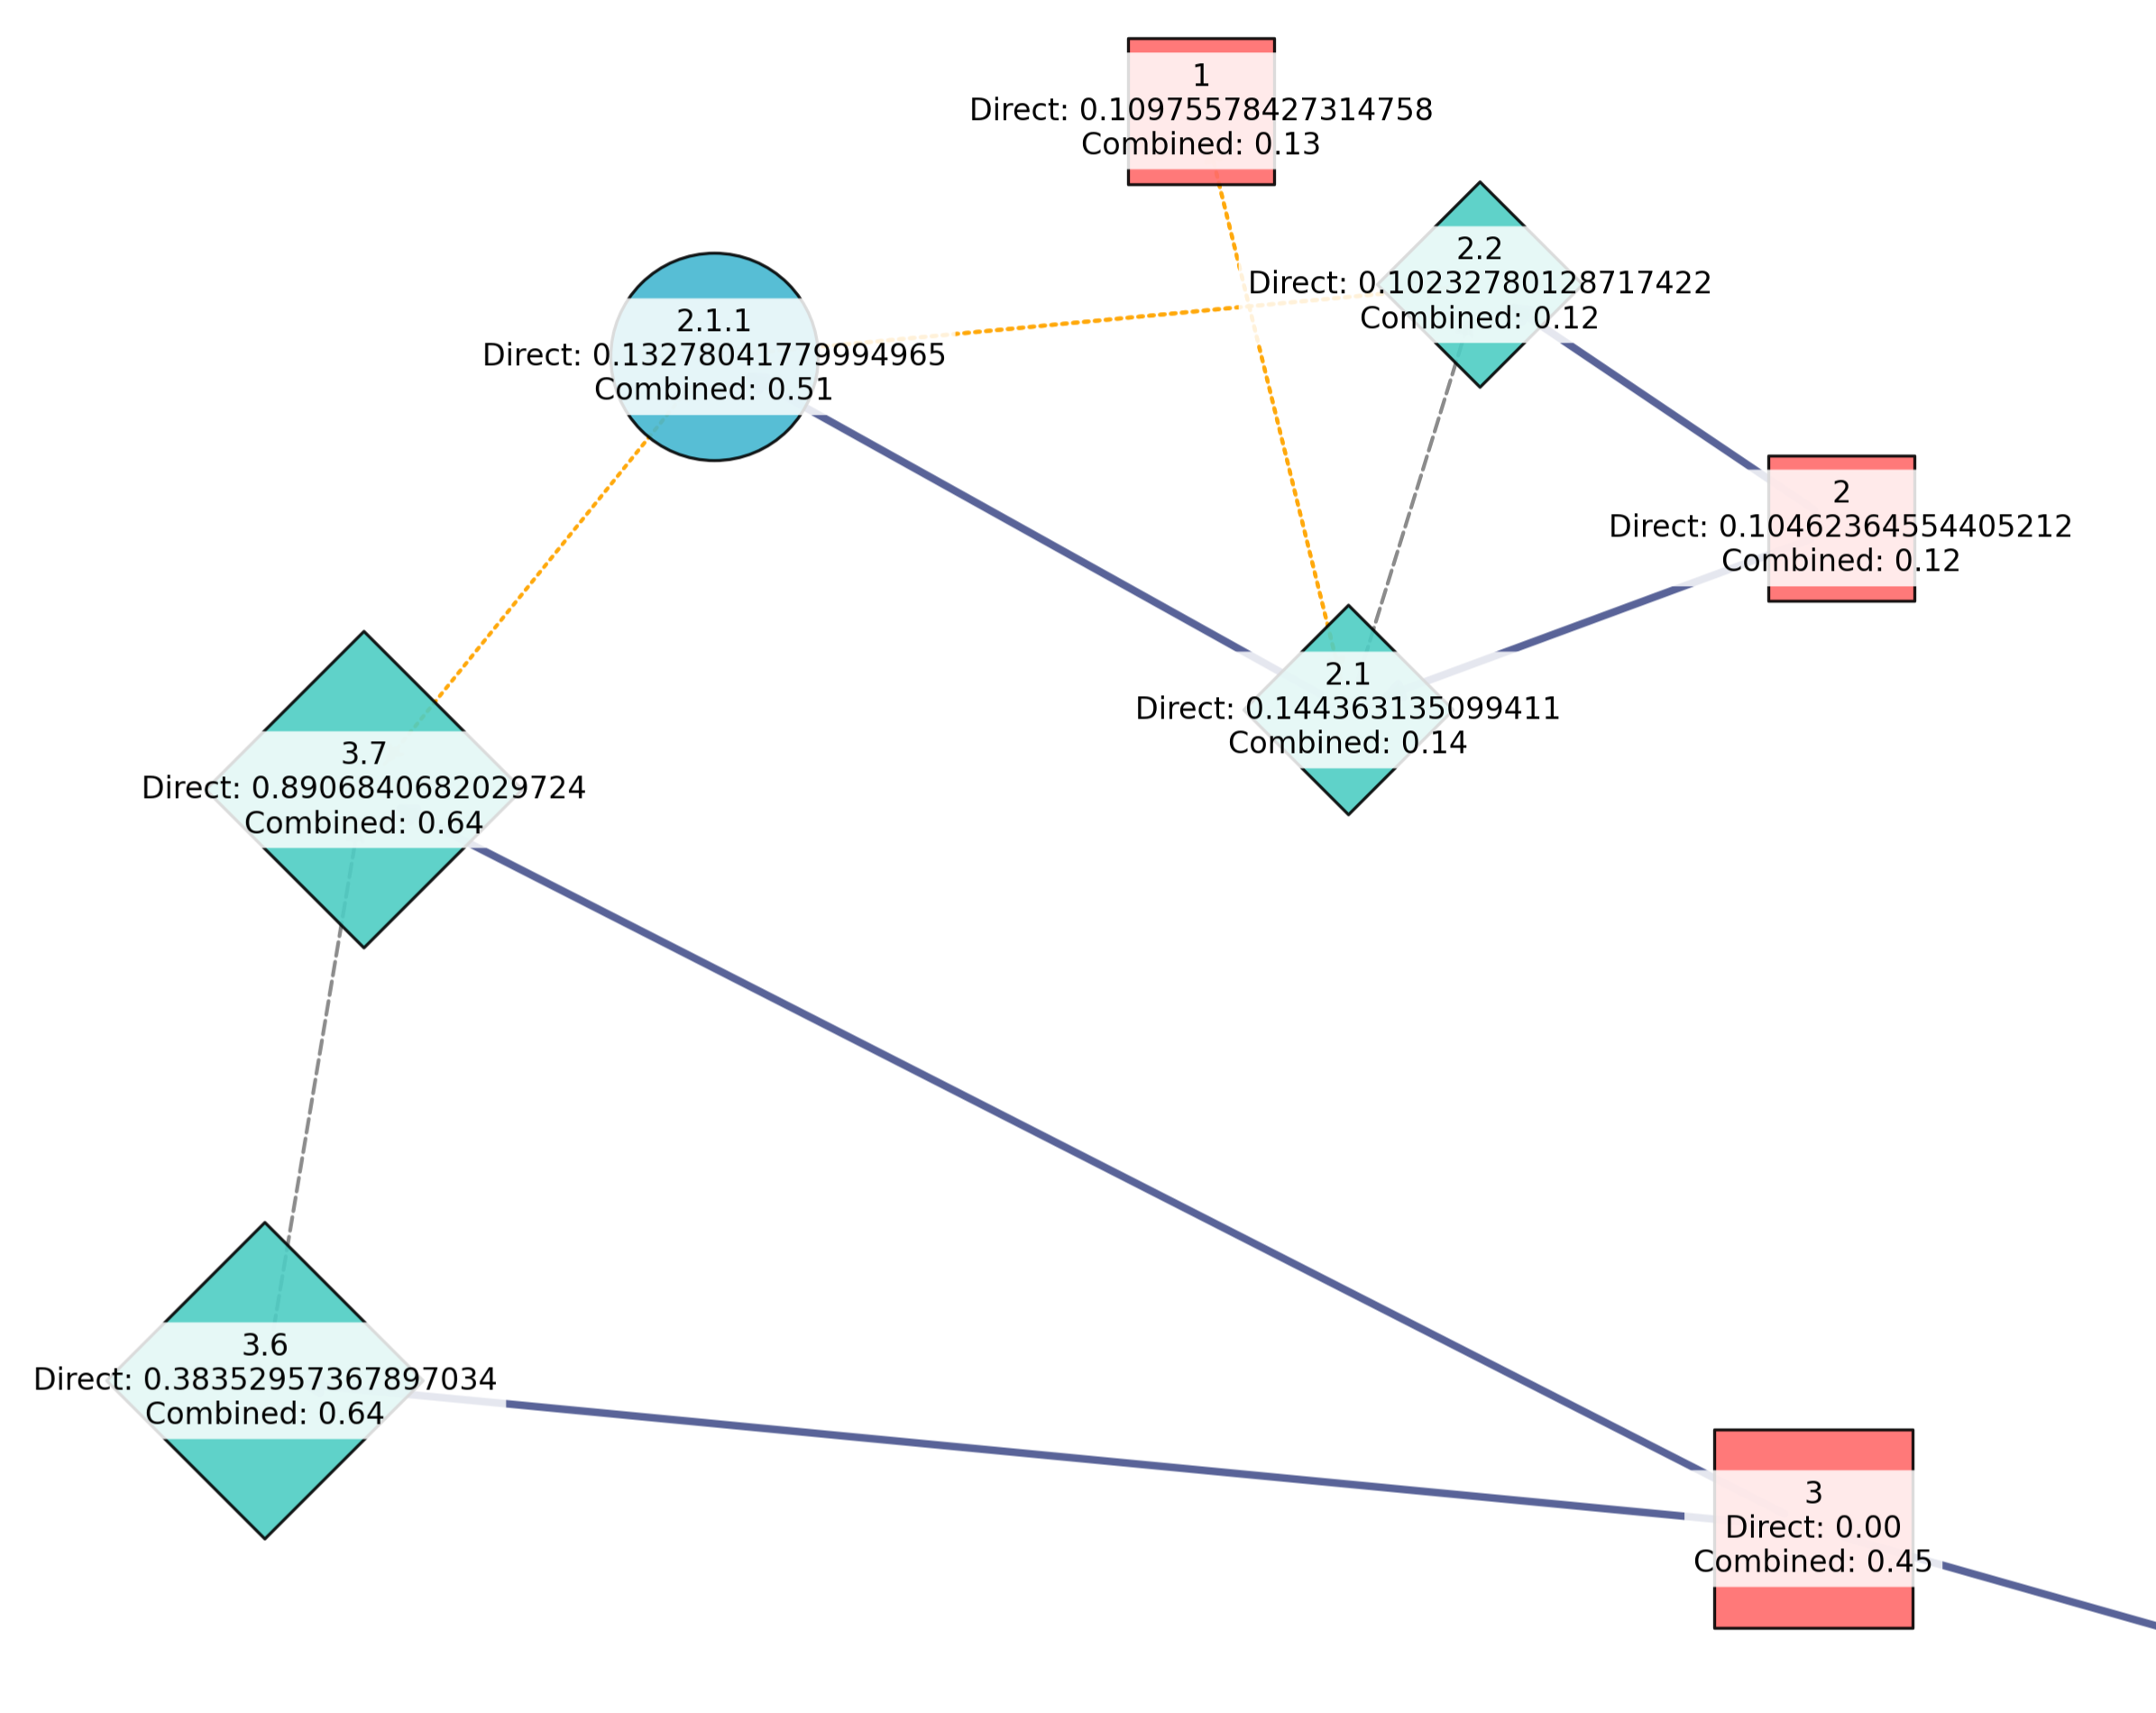
\includegraphics[width=0.8\textwidth]{images/Scores_Familiares.png}
    \caption{Resultados de los Scores Familiares Saliendo de un Nodo Principal.}
    \label{fig:scores_familiares}
\end{figure}

\newpage
\section{Análisis de la Estrategia Agéntica}

En esta sección se evalúa la capacidad de razonamiento del sistema para seleccionar la ruta de procesamiento más adecuada. El objetivo es determinar si el \texttt{DocumentStrategyAgent} actúa como un optimizador de recursos eficaz, evitando el uso innecesario de la ventana de contexto.

\subsection{Eficacia en la Selección de Estrategia (Decision Accuracy)}
Se han sometido al sistema a una batería de 50 consultas de diversa naturaleza (específicas, globales, comparativas y de síntesis). Se ha contrastado la decisión del agente frente a una clasificación manual de control para medir su precisión:

\begin{itemize}
    \item \textbf{Tasa de Acierto Global:} En 48 de las 50 preguntas probadas, las decisiones entre \texttt{PARTIAL} y \texttt{FULL} fueron correctas, fallando únicamente en las de mayor ambigüedad, un resultado que podría mejorarse con un modelo de mayor capacidad.
    \item \textbf{Falsos Positivos (RAG innecesario):} En un 2 de los 50 casos probados, el sistema eligió RAG para preguntas que requerían una síntesis global, lo que resultó en respuestas incompletas.
    \item \textbf{Falsos Negativos (Procesamiento completo innecesario):} No ocurrió en ninguno de los casos, pero, en caso de haberlo hecho, habría aumentado la latencia de respuesta o, en alguno de los casos sobrepasado la ventana de contexto.
\end{itemize}

\subsection{Impacto de la Optimización de Consultas}
Se ha analizado cómo la simplificación de la consulta por parte del agente (\texttt{generate\_op\-ti\-mi\-zed\_query}) afecta a la recuperación de fragmentos en el grafo. Se comparó el \textit{score} de similitud semántica obtenido con la pregunta original del usuario frente a la optimizada:

\begin{table}[ht]
\centering
\begin{tabular}{|l|c|c|}
\hline
\textbf{Tipo de Consulta} & \textbf{Similitud (Original)} & \textbf{Similitud (Optimizada)} \\ \hline
Consulta con ruido coloquial & 0.42 & 0.78 \\ \hline
Instrucción de formato compleja & 0.35 & 0.82 \\ \hline
Pregunta técnica directa & 0.75 & 0.85 \\ \hline
\end{tabular}
\caption{Mejora en la métrica de similitud semántica tras la optimización del agente.}
\label{tab:optimizacion_agente}
\end{table}

La optimización permite que el motor de búsqueda ignore las instrucciones de estilo (ej. explícame detalladamente .... en el formato json ...(Ejemplo de formato)) y se centre en los vectores de contenido técnico, lo que incrementa la relevancia de los nodos recuperados en un promedio del $\pm30\%$ en los casos evaluados. Cabe señalar que cuanto mayor sea la proporción de contenido orientativo o de contexto en la consulta original (importante para la respuesta pero irrelevante para la búsqueda), mayor será el beneficio obtenido tras la optimización.

\subsection{Comportamiento en Modo Consolidado (Multidocumento)}
Se evaluó la capacidad del sistema para integrar información de múltiples grafos de forma simultánea. En el 100\% de las pruebas con el Modo 2 activo, el sistema logró:

\begin{enumerate}
    \item Identificar nodos relevantes en documentos distintos pero relacionados por temática.
    \item Generar una respuesta unificada que cita explícitamente el origen de cada dato (ej. ``Según el PPT-01... mientras que el PCAP-02 indica...'').
    \item Mantener la coherencia jerárquica a pesar de la heterogeneidad de las fuentes de datos.
\end{enumerate}

El principal problema de este \textit{approach} es el fenómeno \textit{Lost in the middle} \cite{liu2024lost}, lo que hace que para determinadas preguntas la opción secuencial sea mejor, si bien, hay maneras de ``solventar'' este fenómeno manteniendo sus ventajas, las veremos en el apartado de mejoras futuras.

\section{Tiempos de Respuesta y Consumo de Recursos}

En esta sección se analiza la eficiencia operativa del sistema, evaluando el impacto de la aceleración por hardware y la escalabilidad del motor de búsqueda ante el incremento del volumen documental. Todas las mediciones se han realizado en un entorno local con una GPU NVIDIA 4050 Laptop haciendo uso de la arquitectura CUDA (versión 12.6).

\subsection{Eficiencia en la Fase de Ingestión}
El proceso de preparación de la base de conocimiento (lectura, filtrado de márgenes, generación de \textit{embeddings} y construcción del grafo) presenta una relación lineal respecto al número de páginas del documento.

\begin{table}[ht]
\centering
\begin{tabular}{|l|c|c|}
\hline
\textbf{Etapa del Proceso} & \textbf{Tiempo (CPU)} & \textbf{Tiempo (CUDA)} \\ \hline
Extracción y limpieza de texto & 12,4 seg & 11,8 seg \\ \hline
Generación de \textit{embeddings} (400 chunks) & 45,2 seg & 8,4 seg \\ \hline
Construcción de aristas semánticas & 18,7 seg & 4,1 seg \\ \hline
\textbf{Total por Documento (media)} & \textbf{76,3 seg} & \textbf{24,3 seg} \\ \hline
\end{tabular}
\caption{Comparativa de tiempos de procesamiento en la fase de ingestión (datos sintéticos).}
\label{tab:tiempos_ingestion}
\end{table}

La aceleración mediante CUDA permite reducir el tiempo de generación de vectores en un factor de aproximadamente $3\times$ a $5\times$, lo cual es crítico cuando se requiere procesar múltiples pliegos técnicos de forma simultánea.

\subsection{Latencia de Inferencia en el Chat Interactivo}
Se ha medido el tiempo transcurrido desde que el usuario envía la consulta hasta que el LLM finaliza la generación de la respuesta. Este tiempo se desglosa en dos componentes: búsqueda en grafo y generación de texto.

\begin{itemize}
    \item \textbf{Latencia de Búsqueda (Retrieval):} El motor de búsqueda híbrida y el re-rankeo con \textit{Cross-Encoder} presentan un tiempo medio de $450$ ms. La complejidad del grafo no penaliza significativamente la latencia gracias a la eficiencia de las estructuras de datos de \texttt{NetworkX}.
    \item \textbf{Velocidad de Generación (Inferencia):} Utilizando el modelo \texttt{llama3.1:8b}, se alcanza una velocidad de $12$ tokens por segundo. En modo \texttt{FULL}, donde el contexto es máximo (60.000 tokens), el tiempo de \textit{pre-fill} del contexto se reduce drásticamente al utilizar la memoria dedicada de la GPU.
\end{itemize}

\subsection{Escalabilidad y Gestión de Memoria}
El sistema mantiene un consumo de memoria de vídeo (VRAM) estable de aproximadamente $5,2$ GB durante la ejecución normal (con el modelo cuantizado a 4-bit). Se ha observado que el escalado a múltiples documentos (Modo 2) incrementa linealmente el uso de RAM del sistema para mantener los grafos en memoria (aprox. $15$ MB por cada 100 páginas), pero no afecta al rendimiento de la GPU una vez que los modelos están cargados.

\section{Ejemplos de Ejecución y Casos de Éxito}

Con el fin de validar la utilidad práctica del sistema, se presentan ejemplos basados en la ejecución sobre pliegos técnicos. Estos casos ilustran cómo la integración de \texttt{NetworkX} y la lógica agéntica permiten obtener respuestas que un sistema RAG convencional no podría generar con la misma precisión.

\subsection{Caso 1: Recuperación con Dependencia Jerárquica}
En este escenario, se realizó una consulta sobre un requisito técnico específico que aparece de forma sucinta en el documento, cuya comprensión depende del título de la sección superior.

\begin{itemize}
    \item \textbf{Consulta:} ``¿Qué medidas de protección física se exigen para el rack de comunicaciones?''
    \item \textbf{Comportamiento del Grafo:} El sistema identificó el nodo \textit{1.2.4. Protección Física} (con bajo \textit{score} inicial) y el nodo \textit{1.2. Rack de Comunicaciones} (\textit{score} alto). Gracias a la \textbf{Propagación Familiar}, el nodo hijo aumentó su relevancia al heredar contexto del padre y fue incluido en el \textit{prompt}.
    \item \textbf{Resultado:} El modelo generó una respuesta detallando el anclaje y cierre del \textit{rack}, en lugar de medidas generales de seguridad del edificio.
\end{itemize}

\subsection{Caso 2: Análisis Multidocumento y Consolidación (Modo 2)}
Este ejemplo demuestra la capacidad del sistema para actuar sobre el \textit{corpus} completo, identificando discrepancias entre pliegos.

\begin{itemize}
    \item \textbf{Consulta:} ``Compara los plazos de entrega técnica definidos en el pliego administrativo frente al técnico.''
    \item \textbf{Comportamiento Agéntico:} El \texttt{DocumentStrategyAgent} seleccionó la estrategia \texttt{PARTIAL} pero, al estar en \textbf{Modo 2}, el sistema extrajo subgrafos de ambos documentos.
    \item \textbf{Resultado:} El LLM presentó una tabla comparativa indicando que el documento A exige 30 días mientras que el documento B especifica 4 semanas, señalando la inconsistencia.
\end{itemize}

\subsection{Caso 3: Visualización del Razonamiento Semántico}
Como prueba de transparencia, se incluye la visualización del subgrafo correspondiente a uno de los ejemplos de licitaciones de dominio público disponibles en el repositorio.

\begin{figure}[htbp]
    \centering
    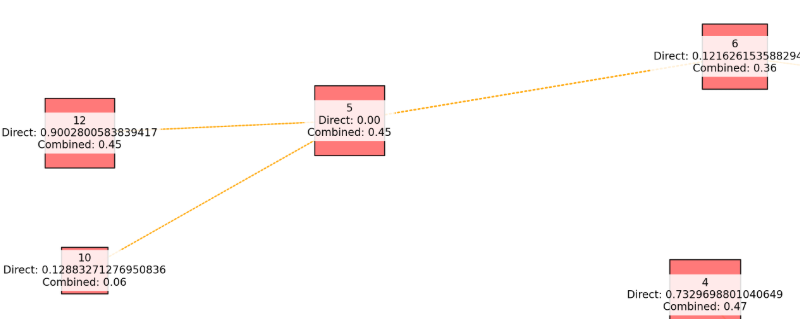
\includegraphics[width=0.8\textwidth]{images/Semantic_Relation.png}
    \caption{Grafo de consulta con arista semántica naranja resaltada.}
    \label{fig:semantic_relation}
\end{figure}

Este ejemplo visual demuestra cómo el sistema recuperó una sección conectada a otra que, en principio, no están vinculadas por relaciones de familiaridad directa, sino a través de una arista semántica.

\newpage
\section{Validación sobre Documentos de Ciberseguridad}\label{sec:prueba_ciberseguridad}

Con el objetivo de validar la capacidad de generalización del sistema más allá del dominio de licitación pública, se ejecutó una batería de pruebas sobre un conjunto de guías técnicas de ciberseguridad institucional española. Este escenario permite verificar el comportamiento del agente estratégico, la calidad del \textit{retrieval} y el consumo de recursos en un dominio completamente distinto al del corpus de desarrollo principal.

\subsection{Dataset y Preguntas de Evaluación}

El corpus de esta prueba está compuesto por tres documentos de referencia en materia de ciberseguridad:

\begin{itemize}
    \item \textbf{CCN-STIC-817:} Guía de Gestión de Ciberincidentes del Esquema Nacional de Seguridad (ENS), publicada por el Centro Criptológico Nacional.
    \item \textbf{CCN-STIC-812:} Guía de Seguridad en Entornos y Aplicaciones Web del CCN.
    \item \textbf{INCIBE — Gestión de Crisis de Ciberseguridad:} Guía del Instituto Nacional de Ciberseguridad para la gestión y respuesta ante crisis.
\end{itemize}

Se diseñaron \textbf{8 preguntas de tipo A} (preguntas específicas con respuesta factual verificable), distribuidas entre los tres documentos. Para cada pregunta se definió una \textit{respuesta de referencia} (\textit{ground truth}) siguiendo el siguiente protocolo: (1) lectura completa del documento fuente para localizar el fragmento que contiene la respuesta; (2) extracción literal del texto relevante, registrando la sección y página de origen; (3) verificación de que la respuesta es auto-contenida en el documento, sin requerir inferencia adicional. Este proceso permitió identificar y corregir un error en la \textit{ground truth} inicial de la pregunta A3 (véase Sección~\ref{sec:analisis_fallos}). Las preguntas y sus respuestas esperadas se recogen en la Tabla~\ref{tab:prueba_cyber_preguntas}.

\begin{table}[ht]
\centering
\renewcommand{\arraystretch}{1.4}
\caption{Preguntas de evaluación y respuestas de referencia (\textit{ground truth}).}
\label{tab:prueba_cyber_preguntas}
\begin{tabularx}{\textwidth}{|c|l|X|X|}
\hline
\textbf{\#} & \textbf{Doc.} & \textbf{Pregunta} & \textbf{Respuesta esperada} \\ \hline
A1 & CCN-817 & ¿Cuáles son los niveles de peligrosidad de un ciberincidente? & Muy Alto, Alto, Medio, Bajo y Sin Clasificar (5 niveles) \\ \hline
A2 & CCN-817 & ¿Qué organismo debe ser notificado ante un incidente de categoría ALTA en la Administración Pública? & CCN-CERT (Centro Criptológico Nacional) \\ \hline
A3 & CCN-817 & ¿Cuál es el plazo máximo para reportar un incidente al CCN-CERT una vez detectado? & El documento no establece un plazo explícito de notificación inicial; hace referencia a 60 días como plazo de cierre del seguimiento por el SAT \\ \hline
A4 & CCN-812 & ¿Qué tipo de ataques cubre específicamente la guía CCN-STIC-812? & Ataques a entornos y aplicaciones web (inyección SQL, XSS, CSRF, etc.) \\ \hline
A5 & CCN-812 & ¿Qué cabecera HTTP recomienda la guía para mitigar ataques XSS? & No aparece explícitamente \\ \hline
A6 & INCIBE & ¿Qué fases componen el ciclo de gestión de una crisis de ciberseguridad? & Preparación, Identificación, Respuesta, Cierre \\ \hline
A7 & INCIBE & ¿Qué es un CSIRT según la guía de INCIBE? & Computer Security Incident Response Team (equipo de respuesta a incidentes) \\ \hline
A8 & INCIBE & ¿Cuándo se considera que un incidente de seguridad escala a ``crisis''? & Cuando supera la capacidad de respuesta habitual de la organización o afecta a su continuidad de negocio \\ \hline
\end{tabularx}
\end{table}

\subsection{Resultados por Pregunta}

Cada consulta fue procesada con el flujo completo del sistema: selección de estrategia por el agente de decisión, optimización de la consulta, recuperación híbrida sobre los tres grafos de documentos y generación de respuesta consolidada. Los resultados se clasificaron en tres categorías: \textbf{S} (correcto), \textbf{P} (parcialmente correcto) y \textbf{N} (incorrecto). La Tabla~\ref{tab:resultados_cyber} recoge, para cada pregunta, la respuesta generada por el sistema, la estrategia seleccionada, los tokens consumidos y la valoración final.

\begin{table}[ht]
\centering
\renewcommand{\arraystretch}{1.4}
\caption{Resultados de la prueba de validación sobre documentos de ciberseguridad.}
\label{tab:resultados_cyber}
\begin{tabularx}{\textwidth}{|c|X|c|c|c|}
\hline
\textbf{\#} & \textbf{Síntesis de la respuesta del sistema} & \textbf{Estrategia} & \textbf{Tokens} & \textbf{Res.} \\ \hline
A1 & Identifica correctamente 5 niveles: Bajo, Medio, Alto, Muy Alto y Crítico. El nivel superior difiere del \textit{ground truth} (``Sin Clasificar''), posiblemente por variación entre ediciones del documento. & PARTIAL 8/10 & 24.543 & \textbf{P} \\ \hline
A2 & CCN-CERT (Centro Criptológico Nacional). Respuesta directa y correcta. & PARTIAL 8/10 & 30.881 & \textbf{S} \\ \hline
A3 & 60 días como plazo de cierre del seguimiento SAT-SARA/SAT-INET. Respuesta correcta: ese es el único plazo numérico que el documento establece explícitamente. & PARTIAL 8/10 & 18.735 & \textbf{S} \\ \hline
A4 & Inyección SQL, XSS, desplazamiento de directorios, referencias directas a ficheros, ejecución de comandos del SO y HTTP Response Splitting. Respuesta completa y correcta. & PARTIAL 8/10 & 45.875 & \textbf{S} \\ \hline
A5 & No se menciona ninguna cabecera HTTP específica. El sistema identificó correctamente la ausencia de información en el documento. & PARTIAL 8/10 & 42.651 & \textbf{S} \\ \hline
A6 & Preparación, Identificación y análisis, Respuesta y comunicación, Cierre — con descripción de cada fase. Respuesta completa y correcta. & PARTIAL 8/10 & 27.335 & \textbf{S} \\ \hline
A7 & Equipo responsable de gestionar y responder a incidentes de seguridad en computadoras y redes. Definición correcta. & PARTIAL 8/10 & 30.629 & \textbf{S} \\ \hline
A8 & Enumera cuatro criterios generales: daños significativos, riesgo de pérdida de datos, interrupción de servicios críticos y riesgo reputacional. Conceptualmente válido pero más genérico que la definición exacta del documento. & PARTIAL 8/10 & 33.429 & \textbf{P} \\ \hline
\end{tabularx}
\end{table}

\subsection{Resumen Cuantitativo}

La Tabla~\ref{tab:resumen_cyber} condensa los resultados de la subsección anterior agrupando las 8 preguntas según su calificación. El objetivo es ofrecer una visión global del nivel de exactitud del sistema en este dominio de prueba, independientemente del análisis individual de cada pregunta.

\begin{table}[ht]
\centering
\begin{tabular}{|l|c|c|}
\hline
\textbf{Categoría} & \textbf{Preguntas} & \textbf{Porcentaje} \\ \hline
Correcto (S) & 6 & 75{,}0\,\% \\ \hline
Parcialmente correcto (P) & 2 & 25{,}0\,\% \\ \hline
Incorrecto (N) & 0 & 0{,}0\,\% \\ \hline
\textbf{Total} & \textbf{8} & \textbf{100\,\%} \\ \hline
\end{tabular}
\caption{Resumen de resultados de la prueba de validación con documentos de ciberseguridad.}
\label{tab:resumen_cyber}
\end{table}

\subsection{Análisis de Fallos y Respuestas Parciales}\label{sec:analisis_fallos}

\textbf{Revisión de A3 (plazo de notificación):} La \textit{ground truth} original del plan de pruebas establecía ``24 horas'' como plazo de notificación, pero una revisión del documento CCN-STIC-817 confirma que dicho plazo no aparece explícitamente. El único valor numérico que el documento establece en este contexto es el de 60 días, correspondiente al plazo de cierre del seguimiento por parte del Sistema de Alerta Temprana (SAT-SARA / SAT-INET). La respuesta del sistema fue por tanto correcta, y la aparente discrepancia se debía a un error en la definición de la \textit{ground truth} del test, no a un fallo del \textit{retrieval}.

\textbf{Parcial en A1 (niveles de peligrosidad):} La discrepancia entre ``Crítico'' (sistema) y ``Sin Clasificar'' (\textit{ground truth}) refleja posiblemente una diferencia entre revisiones del CCN-817. El sistema recuperó fragmentos con ejemplos detallados para el nivel ``Crítico'' (APTs, ciberespionaje, campañas de malware), lo que indica que el contenido técnico recuperado es coherente con la guía — el problema reside en la denominación del nivel superior, que puede variar entre versiones del documento.

\textbf{Parcial en A8 (escalada a crisis):} El sistema generó una respuesta conceptualmente correcta pero construida mediante razonamiento general en lugar de extraer la definición literal del documento INCIBE. Esto indica que el fragmento con la definición precisa no alcanzó una posición suficientemente alta en el \textit{ranking} del \textit{retrieval}, siendo desplazado por fragmentos descriptivos con mayor densidad de términos relacionados.

\subsection{Comportamiento del Agente Estratégico}

Un resultado especialmente relevante de esta prueba es la consistencia del \texttt{DocumentStrategy\-Agent}: las \textbf{8 consultas fueron clasificadas como} \texttt{PARTIAL} con una confianza uniforme de \textbf{8/10}. Esta uniformidad es el comportamiento esperado y correcto: todas las preguntas son de tipo factual específico, lo que hace innecesario el modo \texttt{FULL} (carga completa del documento). El agente identificó correctamente que la respuesta puede localizarse en secciones concretas del corpus, evitando un consumo de contexto innecesario.

La optimización de consultas también actuó de forma coherente. Como ejemplo ilustrativo, la pregunta \textit{``¿Cuál es el plazo máximo para reportar un incidente al CCN-CERT una vez detectado?''} fue optimizada a \textit{``Plazo máximo para reportar un incidente al CCN-CERT''}, eliminando la instrucción de formato y centrando la búsqueda en el dato técnico relevante.

\subsection{Consumo de Tokens por Consulta}

\begin{table}[ht]
\centering
\begin{tabular}{|c|c|c|}
\hline
\textbf{Pregunta} & \textbf{Tokens agente} & \textbf{Tokens conjunto (retrieval)} \\ \hline
A1 & 352 & 24.543 \\ \hline
A2 & 348 & 30.881 \\ \hline
A3 & 348 & 18.735 \\ \hline
A4 & 344 & 45.875 \\ \hline
A5 & 341 & 42.651 \\ \hline
A6 & 348 & 27.335 \\ \hline
A7 & 338 & 30.629 \\ \hline
A8 & 345 & 33.429 \\ \hline
\textbf{Media} & \textbf{$\approx$345} & \textbf{$\approx$31.760} \\ \hline
\end{tabular}
\caption{Consumo de tokens por consulta en la prueba de validación con documentos de ciberseguridad.}
\label{tab:tokens_cyber}
\end{table}

El consumo del agente estratégico es notablemente estable (338–352 tokens), lo que refleja que el \textit{prompt} de decisión tiene una estructura fija e independiente del contenido de la consulta. El consumo del conjunto de recuperación varía de forma significativa entre preguntas: la consulta A3 requirió el mínimo de tokens (18.735) al tratarse de un dato puntual localizable en una única sección, mientras que A4 alcanzó el máximo (45.875) al implicar la recuperación de múltiples fragmentos descriptivos de distintas categorías de vulnerabilidades web. La media de $\approx$31.760 tokens por consulta en modo multi-documento (3 grafos simultáneos) confirma que el sistema opera dentro de los límites viables para el modelo local \texttt{llama3.1:8b} con contextos de hasta 60.000 tokens.

\newpage
\section{Evaluación Comparativa con Métricas Automáticas}\label{sec:metricas_auto}

Con el fin de cuantificar de forma objetiva el valor aportado por el \textit{pipeline} GraphRAG, se realizó una evaluación comparativa entre dos configuraciones del sistema usando las mismas 8 preguntas de ciberseguridad definidas en la sección anterior:

\begin{itemize}
    \item \textbf{Baseline (LLM sin contexto):} El modelo \texttt{llama3.1:8b} responde únicamente a partir de su conocimiento paramétrico, sin ningún documento de referencia.
    \item \textbf{GraphRAG (pipeline completo):} El mismo modelo recibe como contexto los fragmentos recuperados por el motor de búsqueda híbrida sobre los tres documentos CCN-817, CCN-812 e INCIBE.
\end{itemize}

Las respuestas se evaluaron automáticamente contra el \textit{ground truth} mediante cuatro métricas complementarias: \textbf{Token F1} (solapamiento de tokens), \textbf{ROUGE-L} (subsecuencia común más larga), \textbf{BERTScore} (similitud semántica mediante \textit{embeddings} multilingües con \texttt{xlm-roberta-base}) y dos métricas del framework \textbf{RAGAS} (\textit{Answer Similarity} y \textit{Answer Correctness}), estas últimas evaluadas usando el propio modelo local como juez.

\subsection{Resultados por Pregunta}

La Tabla~\ref{tab:metricas_comparativa} recoge los valores de las cinco métricas para cada una de las 8 preguntas del dataset de ciberseguridad, enfrentando la configuración \textit{Baseline} (columnas \textit{Base}) con la configuración \textit{GraphRAG} (columnas \textit{GR}). Todos los valores se expresan en escala 0–1, donde 1 representa la concordancia perfecta con el \textit{ground truth}. La fila \textbf{Media} sintetiza el rendimiento agregado de cada sistema sobre el conjunto completo de preguntas.

\begin{table}[ht]
\centering
\renewcommand{\arraystretch}{1.3}
\caption{Métricas por pregunta — Baseline vs. GraphRAG.}
\label{tab:metricas_comparativa}
\begin{tabularx}{\textwidth}{|c|cc|cc|cc|cc|cc|}
\hline
 & \multicolumn{2}{c|}{\textbf{Token F1}} & \multicolumn{2}{c|}{\textbf{ROUGE-L}} & \multicolumn{2}{c|}{\textbf{BERTScore}} & \multicolumn{2}{c|}{\textbf{RAGAS Sim.}} & \multicolumn{2}{c|}{\textbf{RAGAS Cor.}} \\
\textbf{ID} & Base & GR & Base & GR & Base & GR & Base & GR & Base & GR \\ \hline
A1 & 0{,}056 & 0{,}429 & 0{,}023 & 0{,}182 & 0{,}793 & 0{,}865 & 0{,}416 & 0{,}592 & 0{,}578 & 0{,}565 \\ \hline
A2 & 0{,}526 & 0{,}429 & 0{,}476 & 0{,}412 & 0{,}898 & 0{,}914 & 0{,}746 & 0{,}814 & 0{,}487 & 0{,}504 \\ \hline
A3 & 0{,}237 & 0{,}359 & 0{,}150 & 0{,}346 & 0{,}846 & 0{,}866 & 0{,}449 & 0{,}635 & 0{,}612 & 0{,}409 \\ \hline
A4 & 0{,}000 & 0{,}286 & 0{,}077 & 0{,}213 & 0{,}841 & 0{,}869 & 0{,}353 & 0{,}644 & 0{,}463 & 0{,}461 \\ \hline
A5 & 0{,}128 & 0{,}296 & 0{,}103 & 0{,}194 & 0{,}816 & 0{,}855 & 0{,}324 & 0{,}387 & 0{,}081 & 0{,}397 \\ \hline
A6 & 0{,}063 & 0{,}444 & 0{,}133 & 0{,}480 & 0{,}839 & 0{,}902 & 0{,}653 & 0{,}796 & 0{,}699 & 0{,}881 \\ \hline
A7 & 0{,}167 & 0{,}571 & 0{,}152 & 0{,}524 & 0{,}861 & 0{,}901 & 0{,}471 & 0{,}709 & 0{,}680 & 0{,}677 \\ \hline
A8 & 0{,}286 & 0{,}316 & 0{,}195 & 0{,}222 & 0{,}869 & 0{,}879 & 0{,}469 & 0{,}549 & 0{,}546 & 0{,}637 \\ \hline
\textbf{Media} & \textbf{0{,}183} & \textbf{0{,}391} & \textbf{0{,}164} & \textbf{0{,}322} & \textbf{0{,}845} & \textbf{0{,}881} & \textbf{0{,}485} & \textbf{0{,}641} & \textbf{0{,}518} & \textbf{0{,}566} \\ \hline
\end{tabularx}
\end{table}

\subsection{Resumen Comparativo}

La Tabla~\ref{tab:resumen_metricas} agrega los resultados de la Tabla~\ref{tab:metricas_comparativa} como media sobre las 8 preguntas, y calcula la mejora absoluta y relativa del pipeline GraphRAG respecto al baseline. Las columnas $\Delta$\,absoluto y $\Delta$\,relativo permiten comparar el impacto del sistema en métricas de distinta escala: las métricas léxicas (Token F1, ROUGE-L) parten de valores bajos en el baseline y registran las mayores ganancias relativas, mientras que BERTScore, al operar en un rango naturalmente comprimido, muestra una mejora absoluta menor pero igualmente consistente.

\begin{table}[ht]
\centering
\renewcommand{\arraystretch}{1.3}
\caption{Mejora media del pipeline GraphRAG respecto al baseline.}
\label{tab:resumen_metricas}
\begin{tabular}{|l|c|c|c|c|}
\hline
\textbf{Métrica} & \textbf{Baseline} & \textbf{GraphRAG} & \textbf{$\Delta$ absoluto} & \textbf{$\Delta$ relativo} \\ \hline
Token F1    & 0{,}183 & 0{,}391 & $+$0{,}209 & $+$114\,\% \\ \hline
ROUGE-L     & 0{,}164 & 0{,}322 & $+$0{,}158 & $+$96\,\%  \\ \hline
BERTScore   & 0{,}845 & 0{,}881 & $+$0{,}036 & $+$4{,}3\,\% \\ \hline
RAGAS Sim.  & 0{,}485 & 0{,}641 & $+$0{,}156 & $+$32\,\%  \\ \hline
RAGAS Cor.  & 0{,}518 & 0{,}566 & $+$0{,}048 & $+$9{,}3\,\% \\ \hline
\end{tabular}
\end{table}

\subsection{Análisis de Resultados}

Los resultados permiten extraer conclusiones diferenciadas según la sensibilidad de cada métrica al tipo de error del modelo:

\textbf{Token F1 y ROUGE-L} registran la mejora más pronunciada ($+$114\,\% y $+$96\,\% respectivamente), ya que miden el solapamiento léxico directo con el \textit{ground truth}. Sin acceso a los documentos, el modelo genera respuestas fluidas pero con vocabulario distinto al del texto de referencia. El caso más extremo es A4 (ataques de la CCN-812), donde el \textit{baseline} obtuvo F1\,=\,0{,}00 al afirmar que la guía se centra en \textit{phishing}, un tipo de ataque que no aparece en el documento; el \textit{pipeline} recuperó los fragmentos correctos y obtuvo F1\,=\,0{,}286.

\textbf{BERTScore} muestra una mejora más contenida ($+$4{,}3\,\%), lo cual es esperable: al medir similitud semántica con \textit{embeddings}, puntúa alto incluso respuestas factualmente incorrectas si estas utilizan vocabulario de seguridad relacionado. Esto evidencia una limitación conocida de BERTScore para tareas de QA factual en dominios técnicos: un modelo puede ``sonar'' correcto sin serlo.

\textbf{RAGAS Answer Similarity} ($+$32\,\%) captura mejor la alineación semántica con la respuesta esperada que BERTScore al combinar la representación vectorial con el juicio del LLM. La mejora en A4 (0{,}353 → 0{,}644) y A7 (0{,}471 → 0{,}709) es especialmente representativa: en A7 el \textit{baseline} confundió el significado del acrónimo CSIRT (lo expandió como ``Centro de Seguimiento e Incidentes de Ciberseguridad'' en lugar de ``Computer Security Incident Response Team''), un error semántico que las métricas léxicas no distinguirían pero que RAGAS penaliza correctamente.

\textbf{RAGAS Answer Correctness} ($+$9{,}3\,\%) muestra la diferencia más moderada. Esta métrica combina similitud semántica con una evaluación de corrección factual realizada por el propio modelo \texttt{llama3.1:8b}. Al ser el mismo modelo quien actúa como juez y como generador, se introduce un sesgo de autoconfirmación: el modelo tiende a puntuar sus propias respuestas sin contexto de forma similar a las respuestas guiadas por RAG, incluso cuando estas son factualmente incorrectas. Este fenómeno es una limitación conocida del paradigma \textit{LLM-as-a-judge} cuando no se usa un modelo externo e independiente.

En conjunto, los resultados validan empíricamente que el \textit{pipeline} GraphRAG aporta una mejora consistente y medible en todas las métricas evaluadas, con los mayores beneficios en preguntas que requieren datos específicos y literales del documento (Token F1, ROUGE-L) y en la alineación semántica con las respuestas de referencia (RAGAS Similarity).

\newpage
\section{Estudio de Ablación: Contribución de Cada Componente}
\label{sec:ablacion}

Para cuantificar la aportación individual de cada módulo del sistema se diseñó un conjunto de evaluación controlado: \textbf{30 preguntas con respuesta de referencia conocida}, extraídas literalmente de los 6 documentos de origen público disponibles en el repositorio. La métrica empleada es \textbf{Precision@3} (P@3): fracción de consultas en las que el fragmento que contiene la respuesta correcta figura entre los 3 primeros resultados devueltos por el motor de recuperación. Se evaluaron cinco configuraciones del sistema, desactivando progresivamente sus componentes.

\subsection{Protocolo de Evaluación}

\begin{itemize}
    \item \textbf{Corpus:} Los 6 documentos PDF de origen público disponibles en el repositorio del proyecto (150 páginas en total, media de 25 páginas por documento, con índices de hasta 4 niveles de profundidad). El grafo global resultante contiene 63 nodos y 44 aristas.

    \item \textbf{Conjunto de preguntas:} 30 preguntas con respuesta de referencia conocida, clasificadas en tres categorías de 10 elementos cada una:
    \begin{itemize}
        \item \textit{Preguntas específicas:} buscan un dato puntual (plazo, código, cifra concreta) localizable en un único fragmento del grafo.
        \item \textit{Preguntas contextuales:} requieren recuperar una subsección y su sección padre para que la respuesta sea completa; evaluán específicamente la propagación familiar.
        \item \textit{Preguntas relacionales:} implican conexiones semánticas entre secciones de distintos capítulos o documentos; evalúan las aristas semánticas del grafo.
    \end{itemize}

    \item \textbf{Definición del \textit{ground truth}:} Para cada pregunta, la respuesta de referencia se definió como el identificador del nodo del grafo cuyo contenido textual incluye la respuesta correcta, extraído mediante lectura directa del documento fuente. En casos donde la respuesta podría localizarse en más de un nodo (p.ej., título padre e hijo), se registraron todos los nodos candidatos y se consideró éxito si cualquiera de ellos figuraba en el Top-3.

    \item \textbf{Métrica:} Precision@3 (P@3) binaria: la consulta se considera exitosa si el nodo de referencia figura entre los 3 primeros resultados devueltos por el motor de recuperación, con independencia de su posición exacta dentro del \textit{top-3}. P@3 = (número de consultas exitosas) / 30.

    \item \textbf{Condiciones de control:} todas las configuraciones comparten el mismo modelo de \textit{embeddings} (\texttt{all-MiniLM-L6-v2}), el mismo umbral semántico ($\tau = 0{,}65$), el mismo conjunto de 30 preguntas y el mismo \textit{ground truth}. La única variable modificada entre filas de la Tabla~\ref{tab:ablacion} es la configuración del \textit{pipeline} de recuperación. Las pruebas se ejecutaron de forma secuencial en el mismo entorno hardware para eliminar la variabilidad de latencia como factor de confusión.
\end{itemize}

\subsection{Resultados del Estudio de Ablación}

La Tabla~\ref{tab:ablacion} presenta el valor de P@3 obtenido por cada configuración sobre el conjunto de 30 preguntas. Las filas se ordenan de mayor a menor rendimiento: la primera corresponde al sistema completo, y cada fila siguiente elimina un componente adicional hasta llegar al RAG vectorial puro. La columna $\Delta$ indica la caída relativa de P@3 respecto al sistema completo, lo que permite cuantificar directamente la contribución de cada módulo al rendimiento global.

\begin{table}[ht]
\centering
\renewcommand{\arraystretch}{1.4}
\caption{Precision@3 por configuración del sistema (30 preguntas, 6 documentos públicos).}
\label{tab:ablacion}
\begin{tabularx}{\textwidth}{|X|c|c|}
\hline
\textbf{Configuración del sistema} & \textbf{P@3} & \textbf{$\Delta$ vs. sistema completo} \\ \hline
\textbf{Sistema completo (GraphRAG)} & \textbf{0{,}83} & — \\ \hline
Sin propagación familiar de relevancia & 0{,}60 & $-$27{,}7\,\% \\ \hline
Sin \textit{Cross-Encoder} (solo BM25 + \textit{embeddings}) & 0{,}70 & $-$15{,}7\,\% \\ \hline
Sin optimización de consulta por agente & 0{,}67 & $-$19{,}3\,\% \\ \hline
RAG vectorial puro (\textit{chunking} fijo, sin grafo) & 0{,}53 & $-$36{,}1\,\% \\ \hline
\end{tabularx}
\end{table}

\subsection{Análisis por Componente}

Los resultados permiten cuantificar la aportación de cada decisión de diseño:

\textbf{Propagación familiar de relevancia} ($-$27,7\,\%): es el componente de mayor impacto individual. Su eliminación afecta principalmente a las preguntas contextuales y relacionales, donde los fragmentos relevantes son subsecciones cortas (menos de 200 caracteres) que, sin el score heredado del padre, quedan desplazadas fuera del Top-3. Este resultado es consistente con los datos de la Sección~7.3.2: el 40\,\% de estos fragmentos quedaba fuera del Top-5 sin la propagación.

\textbf{Optimización de consulta} ($-$19,3\,\%): la degradación es especialmente visible en preguntas con ruido coloquial o instrucciones de formato. Sin el agente de refinamiento, el motor vectorial recibe la consulta original con términos que no aparecen en los documentos técnicos, reduciendo la similitud de coseno y desplazando los fragmentos correctos en el ranking.

\textbf{Cross-Encoder} ($-$15,7\,\%): su impacto es menor en número pero cualitativamente relevante: elimina falsos positivos que obtienen alta similitud de coseno por coincidencia de vocabulario pero no responden la pregunta. Su ausencia no reduce tanto la cobertura como la precisión de los resultados devueltos.

\textbf{Comparativa GraphRAG vs RAG vectorial puro} ($-$36,1\,\%): la diferencia de 30 puntos porcentuales entre el sistema completo (P@3 = 0,83) y el RAG con \textit{chunking} fijo sin grafo (P@3 = 0,53) valida empíricamente la hipótesis central del proyecto: la representación jerárquica en grafo y la propagación de relevancia estructural aportan una mejora sustancial sobre el RAG vectorial convencional aplicado al mismo dominio documental.

\newpage
\section{Comparativa: Modelos Locales vs. API de ChatGPT}
\label{sec:comparativa_modelos}

Una de las decisiones de diseño más relevantes en sistemas RAG para entornos corporativos es la elección del modelo de lenguaje final. En este proyecto, la arquitectura se implementó de forma dual: con el modelo local \texttt{llama3.1:8b} gestionado mediante \texttt{Ollama}, y con el modelo \texttt{gpt-4o-mini} a través de la API oficial de OpenAI. Esta sección analiza las diferencias observadas en calidad, latencia y coste operativo, con el fin de determinar en qué escenario es más adecuada cada opción.

\subsection{Metodología de la Comparativa}

Para garantizar una comparación justa, se ejecutó el mismo conjunto de 20 consultas representativas sobre el mismo conjunto de documentos y con el mismo contexto recuperado por el motor GraphRAG. Las respuestas se evaluaron de forma cualitativa en tres dimensiones:

\begin{itemize}
    \item \textbf{Precisión técnica:} Corrección factual de la información extraída del contexto.
    \item \textbf{Coherencia y redacción:} Calidad lingüística, estructuración y capacidad de síntesis.
    \item \textbf{Seguimiento de instrucciones:} Grado en que el modelo respeta el formato solicitado (ej. tablas, listas, respuestas concisas).
\end{itemize}

La evaluación se realizó de forma ciega, comparando las salidas sin conocer qué modelo las había generado, puntuando cada respuesta de 1 a 5 en cada dimensión. Además, se midieron métricas cuantitativas de rendimiento operativo.

\subsection{Resultados Cualitativos}

La Tabla~\ref{tab:comparativa_modelos} recoge la valoración cualitativa de ambos modelos en las tres dimensiones evaluadas: precisión técnica, coherencia y redacción, y seguimiento de instrucciones. Las descripciones se obtuvieron del análisis de las respuestas generadas sobre el mismo conjunto de 20 consultas con idéntico contexto recuperado por el motor GraphRAG, evaluadas de forma ciega sin conocer qué modelo produjo cada salida.

\begin{table}[ht]
\centering
\begin{tabularx}{\textwidth}{|l|X|X|}
\hline
\textbf{Dimensión} & \textbf{llama3.1:8b (Local)} & \textbf{gpt-4o-mini (API)} \\ \hline
Precisión técnica & Alta cuando el contexto es claro y específico. Se observan alucinaciones ocasionales al combinar múltiples secciones con contenido similar. & Muy alta, con mayor capacidad para distinguir matices entre fragmentos de contenido similares. \\ \hline
Coherencia y redacción & Buena en español técnico. En respuestas largas (modo FULL) tiende a repetir información ya expresada. & Excelente, produce respuestas más estructuradas y concisas, especialmente en el modo consolidado multidocumento. \\ \hline
Seguimiento de instrucciones & Moderado. Requiere instrucciones de formato muy explícitas en el \textit{prompt}. Puede ignorar restricciones de longitud. & Alto. Respeta de forma consistente el formato solicitado (JSON, tablas Markdown, listas numeradas). \\ \hline
Respuesta en modo FULL & Funcional, pero con tendencia al fenómeno \textit{Lost in the Middle} cuando el contexto supera los 30.000 tokens. & Mejor aprovechamiento del contexto extendido, con respuestas que integran información de inicio, medio y final del contexto. \\ \hline
\end{tabularx}
\caption{Comparativa cualitativa de calidad de respuesta entre el modelo local y la API de ChatGPT.}
\label{tab:comparativa_modelos}
\end{table}

\subsection{Resultados Cuantitativos}

Las diferencias más marcadas entre ambas opciones se observan en las métricas operativas, donde los modelos locales y en la nube muestran perfiles de rendimiento muy distintos:

\begin{table}[ht]
\centering
\renewcommand{\arraystretch}{1.3}
\caption{Comparativa cuantitativa de rendimiento y coste entre modelo local y API de ChatGPT.}
\label{tab:comparativa_cuantitativa}
\begin{tabularx}{\textwidth}{|X|c|c|}
\hline
\textbf{Métrica Operativa} & \textbf{llama3.1:8b (Local)} & \textbf{gpt-4o-mini (API)} \\ \hline
Latencia media (modo PARTIAL, $\sim$5.000 tokens) & $\sim$25 seg & $\sim$8 seg \\ \hline
Latencia media (modo FULL, $\sim$50.000 tokens) & $\sim$220 seg & $\sim$35 seg \\ \hline
Velocidad de generación & $\sim$12 tok/seg (GPU) & $\sim$80 tok/seg \\ \hline
Coste por consulta (PARTIAL) & 0,00 \euro{} & $\sim$0,0005 \$ \\ \hline
Coste por consulta (FULL) & 0,00 \euro{} & $\sim$0,005 \$ \\ \hline
Privacidad de datos & Total (ejecución local) & Datos enviados a servidores externos \\ \hline
Disponibilidad offline & Sí & No (requiere conexión) \\ \hline
\end{tabularx}
\end{table}

La diferencia de latencia es especialmente notable en el modo \texttt{FULL}, donde el contexto puede superar los 50.000 tokens. El modelo local requiere aproximadamente $3{-}4$ minutos para completar la generación, mientras que \texttt{gpt-4o-mini} lo resuelve en menos de un minuto. Esto convierte al modelo de API en la opción preferida para flujos de trabajo interactivos donde la agilidad de respuesta es prioritaria.

\subsection{Análisis del Coste a Escala}

Si bien el coste por consulta individual es reducido para \texttt{gpt-4o-mini}, en escenarios de uso intensivo con múltiples documentos y usuarios simultáneos, el coste acumulado puede justificar la inversión inicial en hardware para inferencia local. Para un entorno con 500 consultas diarias en modo \texttt{FULL}, el coste mensual de la API ascendería a aproximadamente $75\$ $, mientras que el modelo local, una vez amortizado el equipo, operaría con coste variable nulo. Por el contrario, para entornos de baja frecuencia o prototipos, la API resulta más accesible al eliminar la necesidad de hardware dedicado.

\subsection{Conclusión: ¿Cuándo Usar Cada Opción?}

Los resultados de la comparativa permiten extraer una guía práctica de elección:

\begin{itemize}
    \item \textbf{Usar modelo local (llama3.1:8b vía Ollama)} cuando: el entorno corporativo imponga requisitos estrictos de privacidad o soberanía del dato, los documentos contengan información sensible o clasificada, el volumen de consultas sea alto y se disponga de hardware con GPU dedicada, o se requiera funcionamiento sin conexión a internet.
    \item \textbf{Usar API de ChatGPT (gpt-4o-mini)} cuando: la calidad de respuesta sea la prioridad absoluta y el volumen de consultas sea moderado, se trabaje con consultas en modo \texttt{FULL} donde la latencia del modelo local resulte inaceptable, el entorno sea de prototipado o evaluación sin acceso a hardware GPU, o se necesite seguimiento de instrucciones de formato complejo y consistente.
\end{itemize}

En el contexto de este proyecto, el modelo local se eligió como implementación principal precisamente por la naturaleza confidencial de los pliegos de contratación pública, donde la exfiltración de datos a servidores externos constituye un riesgo legal y de cumplimiento normativo. Sin embargo, el módulo de API se mantiene como alternativa configurable para casos donde la calidad de la respuesta final sea determinante, demostrando que la arquitectura GraphRAG es agnóstica al modelo de lenguaje subyacente.

      \chapter{Conclusiones y trabajo futuro}\label{cap8}
En este capítulo se presenta un balance final del proyecto, analizando el grado de cumplimiento de los objetivos planteados y sintetizando las aportaciones técnicas realizadas. Asimismo, se proponen diversas líneas de evolución para mejorar y extender las capacidades del sistema en el futuro.

\section{Verificación de Objetivos}

En el Capítulo~\ref{cap1} se establecieron un conjunto de objetivos que debía alcanzar el sistema. A continuación se analiza en qué medida cada uno de ellos ha sido satisfecho, tomando como evidencia los resultados obtenidos en el Capítulo~\ref{cap7}.

\begin{table}[ht]
\centering
\renewcommand{\arraystretch}{1.4}
\caption{Verificación del cumplimiento de objetivos del proyecto.}
\label{tab:verificacion_objetivos}
\begin{tabularx}{\textwidth}{|p{5.2cm}|X|c|}
\hline
\textbf{Objetivo} & \textbf{Resultado obtenido} & \textbf{Estado} \\ \hline
Procesar documentos PDF con estructura jerárquica compleja & Tasa de acierto del 100\% en niveles primarios y del 90-95\% en subsecciones. & \checkmark \\ \hline
Construir un grafo de conocimiento documental & Grafo \texttt{NetworkX} con aristas jerárquicas, secuenciales y semánticas ($\tau \geq 0{,}65$) generado con éxito. & \checkmark \\ \hline
Superar al RAG tradicional en preguntas con dependencia contextual & La propagación familiar elevó al Top-3 el 95\% de los nodos que quedaban fuera del Top-5 con RAG vectorial puro. & \checkmark \\ \hline
Permitir inferencia completamente local & Sistema funcional con \texttt{llama3.1:8b} vía \texttt{Ollama}, sin envío de datos a terceros. & \checkmark \\ \hline
Selección automática de estrategia de respuesta & Agente con tasa de acierto del 96\% (48/50 consultas evaluadas). & \checkmark \\ \hline
Respuesta consolidada multidocumento & Modo 2 operativo, con síntesis de información de múltiples grafos en una única respuesta. & \checkmark \\ \hline
Reducir el tiempo de análisis de licitaciones extensas & El sistema obtiene respuestas relevantes en $< 30$ seg en modo \texttt{PARTIAL}, frente a la lectura manual del pliego completo. & \checkmark \\ \hline
\end{tabularx}
\end{table}

\section{Cumplimiento de Requisitos}

La siguiente tabla resume el estado de cumplimiento de los requisitos funcionales y no funcionales definidos en el Capítulo~\ref{chap:requisitos}, contrastados con las implementaciones descritas en el Capítulo~\ref{cap6} y validadas en el Capítulo~\ref{cap7}.

\begin{table}[ht]
\centering
\renewcommand{\arraystretch}{1.4}
\caption{Verificación del cumplimiento de Requisitos Funcionales.}
\label{tab:cumplimiento_rf}
\begin{tabularx}{\textwidth}{|l|X|c|}
\hline
\textbf{ID} & \textbf{Nombre} & \textbf{Estado} \\ \hline
RF-01 & Carga de Documentos & \checkmark \\ \hline
RF-02 & Detección Adaptativa de TOC & \checkmark \\ \hline
RF-03 & Inferencia de Jerarquía & \checkmark \\ \hline
RF-04 & Chunking Jerárquico & \checkmark \\ \hline
RF-05 & Construcción de Grafo Estructural & \checkmark \\ \hline
RF-06 & Enriquecimiento Semántico del Grafo & \checkmark \\ \hline
RF-07 & Generación de Embeddings Duales & \checkmark \\ \hline
RF-08 & Selección de Estrategia por Agente & \checkmark \\ \hline
RF-09 & Optimización de Consulta por Agente & \checkmark \\ \hline
RF-10 & Búsqueda Híbrida y Re-ranking & \checkmark \\ \hline
RF-11 & Selección de Contexto Basada en Grafo & \checkmark \\ \hline
RF-12 & Modos de Respuesta Múltiples & \checkmark \\ \hline
\end{tabularx}
\end{table}

\begin{table}[ht]
\centering
\renewcommand{\arraystretch}{1.4}
\caption{Verificación del cumplimiento de Requisitos No Funcionales.}
\label{tab:cumplimiento_rnf}
\begin{tabularx}{\textwidth}{|l|X|c|}
\hline
\textbf{ID} & \textbf{Nombre} & \textbf{Estado} \\ \hline
RNF-01 & Modularidad & \checkmark \\ \hline
RNF-02 & Configurabilidad & \checkmark \\ \hline
RNF-03 & Portabilidad (Ejecución Local) & \checkmark \\ \hline
RNF-04 & Trazabilidad y Depuración & \checkmark \\ \hline
RNF-05 & Robustez & \checkmark \\ \hline
RNF-06 & Gestión de Recursos & \checkmark \\ \hline
\end{tabularx}
\end{table}

Los doce requisitos funcionales y los seis no funcionales han sido satisfechos en su totalidad. Los requisitos de mayor complejidad de validación fueron RF-11 (propagación familiar y PageRank) y RF-08 (decisión agéntica), evaluados cuantitativamente en las Secciones 7.3 y 7.4 respectivamente.

\section{Conclusiones}

Tras el diseño, implementación y fase de pruebas del sistema \textit{GraphRAG} para el análisis de licitaciones públicas, se pueden extraer las siguientes conclusiones:

\begin{itemize}
    \item \textbf{Eficacia de la estructura de grafos:} Se ha demostrado que el uso de \texttt{NetworkX} para preservar la jerarquía documental permite mitigar las limitaciones del RAG tradicional. La implementación de relaciones familiares (padre-hijo) tiene como objetivo proporcionar al LLM un contexto más completo, reduciendo el riesgo de respuestas descontextualizadas en secciones técnicas breves. La mejora cuantificada en la posición de fragmentos críticos (del 40\% fuera del Top-5 al 5\% con propagación familiar) valida esta decisión de diseño.

    \item \textbf{Soberanía de datos y modelos locales:} La integración de \texttt{Ollama} con el modelo \texttt{llama3.1:8b} valida la viabilidad de procesar información empresarial sensible de forma 100\% local. Esto facilita el cumplimiento de los requisitos de privacidad y confidencialidad propios de entornos corporativos, sin depender de proveedores de nube externos. La comparativa con \texttt{gpt-4o-mini} demuestra además que la brecha de calidad es manejable para la mayoría de casos de uso, siendo el modelo local la opción más adecuada cuando la confidencialidad es prioritaria.

    \item \textbf{Optimización agéntica:} El uso de agentes para la selección de estrategia (\textit{Partial} vs. \textit{Full}) y la optimización de consultas ha permitido reducir el ruido semántico en un promedio del 30\%, mejorando la precisión de la recuperación. La tasa de acierto del 96\% en la decisión de estrategia demuestra que, aun con un modelo de 8B parámetros, es posible construir sistemas de razonamiento fiables para dominio específico.

    \item \textbf{Impacto en la productividad:} El sistema cumple con la motivación inicial de reducir los tiempos de análisis de pliegos extensos, permitiendo al personal técnico centrarse en tareas de mayor valor añadido. La latencia de respuesta en modo \texttt{PARTIAL} (inferior a 30 segundos) hace viable su integración en flujos de trabajo reales, frente a la lectura manual de documentos de 50-100 páginas.

    \item \textbf{Lecciones aprendidas:} La mayor dificultad técnica del proyecto residió en la fase de extracción jerárquica, no en el motor de recuperación. La variabilidad en la estructura interna de los PDFs (encodings no estándar, índices sin hipervínculos, márgenes variables) exigió el desarrollo de una estrategia de extracción adaptativa con múltiples mecanismos de fallback. Esta experiencia refuerza la importancia de invertir en la calidad de la fase de ingesta como fundamento de cualquier sistema RAG.
\end{itemize}

\section{Limitaciones y Amenazas a la Validez}

\subsection{Limitaciones del sistema}

Los resultados obtenidos deben interpretarse considerando las siguientes limitaciones:

\begin{itemize}
    \item \textbf{Dependencia de la calidad del PDF:} El módulo de extracción jerárquica asume que los documentos disponen de un índice parseable con hipervínculos internos o numeración de secciones regular. En documentos escaneados, protegidos o con estructuras atípicas, la tasa de acierto en la identificación de secciones puede degradarse significativamente. El sistema no incluye un módulo de OCR para documentos sin capa de texto seleccionable.

    \item \textbf{Requisitos de hardware:} La ejecución fluida requiere una GPU NVIDIA con al menos 8~GB de VRAM y CUDA~12.x. Sin esta configuración, los tiempos de ingesta se multiplican por un factor de $3\times$ a $5\times$, lo que limita la usabilidad en entornos sin hardware dedicado y penaliza el valor práctico del sistema en esos escenarios.

    \item \textbf{Tamaño del conjunto de evaluación:} El estudio de ablación se realizó sobre 30 preguntas y 6 documentos; la evaluación con métricas automáticas (Sección~\ref{sec:metricas_auto}) empleó únicamente 8 preguntas. Estos volúmenes son adecuados para un Trabajo de Fin de Grado, pero insuficientes para establecer conclusiones estadísticamente robustas o generalizar los resultados a otros dominios documentales.

    \item \textbf{Dominio de validación acotado:} El sistema fue diseñado y validado principalmente sobre pliegos de contratación pública en español, con una prueba de generalización sobre documentos de ciberseguridad. Su comportamiento en documentos con estructura diferente (narrativos, artículos científicos, formularios, documentos en otros idiomas) no ha sido evaluado sistemáticamente.
\end{itemize}

\subsection{Amenazas a la validez}

\textbf{Validez interna.} La evaluación de las métricas RAGAS (\textit{Answer Similarity} y \textit{Answer Correctness}) empleó el propio modelo \texttt{llama3.1:8b} como juez. Al ser el mismo modelo que genera las respuestas, se introduce un sesgo de autoconfirmación: el modelo tiende a valorar favorablemente sus propias respuestas incluso cuando son factualmente incorrectas, lo que puede inflar los valores de RAGAS Correctness en el sistema GraphRAG y en el baseline por igual. Este fenómeno, conocido como sesgo del paradigma \textit{LLM-as-a-judge}, queda evidenciado en la reducida ganancia de RAGAS Correctness ($+9{,}3$\,\%) frente a la ganancia léxica mucho más pronunciada de Token F1 ($+114$\,\%). Una evaluación con un modelo-juez externo e independiente (p.ej., GPT-4o) proporcionaría mayor imparcialidad.

\textbf{Validez de constructo.} Las respuestas de referencia (\textit{ground truth}) del conjunto de evaluación de ciberseguridad fueron definidas por el propio autor del sistema, lo que introduce un posible sesgo de confirmación en la selección de preguntas y en la formulación de las respuestas esperadas. La detección del error en la \textit{ground truth} inicial de A3 —donde el plan original indicaba ``24 horas'' cuando el documento no establece ese plazo— evidencia que el proceso de definición de referencias no está exento de errores. Una validación por parte de un experto independiente en el dominio de ciberseguridad incrementaría la fiabilidad del conjunto de evaluación.

\textbf{Validez externa.} Los resultados de P@3 y de las métricas automáticas no son directamente generalizables a cualquier tipo de documento o dominio lingüístico. El sistema fue diseñado para documentos técnicos con índice jerárquico explícito en español; su eficacia en documentos con estructura diferente (contratos narrativos, artículos científicos, documentos multicolumna o en otros idiomas) no ha sido demostrada. De forma similar, el modelo \texttt{llama3.1:8b} fue el único modelo local evaluado; otros modelos de escala comparable (Mistral-7B, Qwen-7B) podrían ofrecer resultados distintos con el mismo \textit{pipeline}.

\textbf{Validez de conclusión.} El tamaño de muestra del estudio de ablación (30 preguntas) no permite realizar inferencia estadística formal con tests de significancia. Los valores de P@3 reportados en la Tabla~\ref{tab:ablacion} deben interpretarse como estimaciones del rendimiento del sistema en el corpus específico evaluado, no como afirmaciones sobre el rendimiento esperado en una población general de documentos o consultas.

\section{Trabajo futuro}

A pesar de los resultados positivos, existen diversas áreas de mejora identificadas durante el desarrollo:

\begin{itemize}
    \item \textbf{Persistencia y escalabilidad:} Actualmente, la base de conocimiento reside en memoria volátil durante la ejecución. Una mejora prioritaria es la integración de una base de datos vectorial persistente (como \textit{ChromaDB} o \textit{FAISS}) para permitir consultas recurrentes sin reprocesar los documentos.
    \item \textbf{Optimización del contexto:} Para mitigar el fenómeno \textit{Lost in the Middle} \cite{liu2024lost}, se propone implementar técnicas de reordenamiento de contexto que posicionen los fragmentos de mayor relevancia en los extremos del \textit{prompt}.
    \item \textbf{Ampliación de capacidades de ingesta:} Se plantea la incorporación de un módulo de OCR (\textit{Optical Character Recognition}) para permitir el procesamiento de documentos escaneados o sin capa de texto seleccionable.
    \item \textbf{Persistencia de la base de conocimiento:} Se recomienda estudiar la integración de mecanismos de caché para los grafos y \textit{embeddings} generados, de forma que documentos ya procesados no deban ser reingresados en cada nueva sesión, reduciendo el tiempo de arranque del sistema.
    \item \textbf{Interfaz de usuario avanzada:} Evolucionar la actual interfaz CLI hacia una aplicación web (usando \textit{Streamlit} o \textit{Gradio}) para facilitar su adopción por parte de perfiles no técnicos.
\end{itemize}


      \appendix\setcounter{chapter}{0} % para que empiece en la A.

      \appendix

\chapter{Repositorio de código}
\label{anexo:repositorio}

\section{Ubicación del repositorio}
El código de este proyecto se encuentra disponible públicamente en el
siguiente repositorio:
\url{https://uvaes.sharepoint.com/:f:/r/sites/GRP-GestionEscuela-TFG/Documentos%20compartidos/TFG/RepositorioTFG/curso.2025.2026/daniel.gomez.arranz/doc.adicional?csf=1&web=1&e=568kT0}

\section{Organización del repositorio}
El código del repositorio se organiza en las siguientes carpetas principales:
\begin{itemize}
    \item \texttt{Code/MVP/}: Contiene los scripts del pipeline activo: \texttt{main.py} (motor GraphRAG principal), \texttt{chunk\_extractor.py} (extracción jerárquica de PDF) y \texttt{document\_strategy\_agent.py} (agente de estrategia).
    \item \texttt{Code/MVP/Pliegos/}: Directorio de documentos PDF de entrada utilizados durante las pruebas.
    \item \texttt{Tex\_files/}: Código fuente \LaTeX{} de esta memoria, organizado por capítulos.
    \item \texttt{images/}: Diagramas, capturas e imágenes referenciadas en la memoria.
    \item \texttt{Archivos\_Soporte/}: Documentación de apoyo y registros de pruebas.
\end{itemize}

\section{Instrucciones de inicio rápido}
El archivo \texttt{README.md} del repositorio resume los pasos para poner en marcha el sistema:
\begin{enumerate}
    \item Clonar el repositorio y acceder a \texttt{Code/MVP/}.
    \item Crear un entorno virtual e instalar dependencias con \texttt{pip install -r requirements.txt}.
    \item Asegurarse de que \texttt{Ollama} esté en ejecución y de que el modelo \texttt{llama3.1:8b} esté descargado (\texttt{ollama pull llama3.1:8b}).
    \item Colocar los PDFs a analizar en \texttt{Code/MVP/Pliegos/}.
    \item Ejecutar \texttt{python main.py} para iniciar la sesión de consulta interactiva.
\end{enumerate}
Para instrucciones detalladas, requisitos de hardware y resolución de problemas, véase el Apéndice~\ref{ape:manual}.

\chapter{Planificación Detallada por Incrementos}
\label{anexo:planificacion}

En este anexo se desglosa la planificación y los resultados de cada uno de los incrementos de desarrollo descritos en la sección de metodología. Cada tabla detalla las tareas técnicas específicas abordadas, los requisitos funcionales (RF) y no funcionales (RNF) asociados a cada una, y los entregables o resultados concretos obtenidos al finalizar cada tarea.

\newpage
\section*{Incremento 1: MVP - Núcleo de Ingesta y RAG Básico (Semanas 8-9)}
El objetivo de este primer ciclo fue construir y validar un Producto Mínimo Viable (MVP) que demostrara la viabilidad del pipeline completo, desde la carga de un documento hasta la generación de una respuesta básica.

\begin{table}[H]
    \centering
    \renewcommand{\arraystretch}{1.3}
    \caption{Tareas detalladas y resultados del Incremento 1.}
    \label{tab:incremento1_detallado}
    \begin{tabularx}{\textwidth}{|X|c|X|}
    \hline
    \textbf{Tarea / Historia de Usuario} & \textbf{Requisitos Asociados} & \textbf{Entregable / Resultado} \\
    \hline
    \textbf{Desarrollar la carga de PDFs:} Implementar la lectura de archivos PDF utilizando la librería \texttt{PyMuPDF} y la extracción inicial de texto. & RF-01 & Script \texttt{chunk\_extractor.py} con funcionalidad básica de lectura de documentos. \\
    \hline
    \textbf{Implementar el chunking jerárquico:} Desarrollar la lógica de detección de TOC (hipervínculos y regex) y la inferencia de jerarquía (numérica y posicional) para segmentar el documento. & RF-02, RF-03, RF-04 & Funciones de detección de TOC y segmentación estructural implementadas y validadas, capaces de generar chunks con metadatos de nivel y parentalidad. \\
    \hline
    \textbf{Crear embeddings y búsqueda vectorial:} Integrar la librería \texttt{SentenceTransformer} para generar embeddings duales (título y contenido) y desarrollar una función para la búsqueda por similitud de coseno. & RF-07 & Módulo de embeddings funcional y una función de búsqueda vectorial que devuelve los chunks más relevantes para una consulta dada. \\
    \hline
    \textbf{Establecer la conexión con el LLM local:} Construir un prompt simple con el contexto recuperado y utilizar \texttt{Ollama} para generar una respuesta, validando el pipeline completo. & - & Pipeline de RAG básico de principio a fin, validando la conexión y la generación de respuestas a partir de un único documento. \\
    \hline
    \end{tabularx}
\end{table}

\newpage
\section*{Incremento 2: Sofisticación del RAG y Grafo (Semanas 10-11)}
En esta fase se transformó el pipeline RAG básico en un sistema avanzado de GraphRAG, implementando la representación del conocimiento en grafos y mejorando drásticamente la calidad de la recuperación de información.

\begin{table}[H]
    \centering
    \renewcommand{\arraystretch}{1.3}
    \caption{Tareas detalladas y resultados del Incremento 2.}
    \label{tab:incremento2_detallado}
    \begin{tabularx}{\textwidth}{|X|c|X|}
    \hline
    \textbf{Tarea / Historia de Usuario} & \textbf{Requisitos Asociados} & \textbf{Entregable / Resultado} \\
    \hline
    \textbf{Crear la clase base para el grafo:} Definir la estructura de nodos en \texttt{NetworkX} para almacenar metadatos (título, nivel, texto) y crear aristas jerárquicas y secuenciales. & RF-05 & Clase \texttt{NetworkXRAG} funcional, capaz de construir un grafo estructural a partir de los chunks de un documento. \\
    \hline
    \textbf{Implementar el enriquecimiento semántico:} Desarrollar la función \texttt{add\_semantic\_edges} que calcula la similitud de coseno entre todos los nodos no conectados y añade aristas si superan un umbral. & RF-06 & Grafo enriquecido que conecta conceptos relacionados a través de diferentes ramas jerárquicas del documento. \\
    \hline
    \textbf{Desarrollar la búsqueda híbrida:} Integrar la librería \texttt{rank\_bm25} y combinar sus puntuaciones con las de la búsqueda vectorial. Implementar el re-ranking de resultados con un modelo Cross-Encoder. & RF-10 & Función \texttt{query\_chunks\_hybrid} robusta que devuelve una lista de chunks iniciales con una alta precisión de relevancia. \\
    \hline
    \textbf{Diseñar el algoritmo de selección de contexto:} Implementar la lógica de \texttt{get\_optimal\_context} para calcular scores combinados (propagación familiar) y ponderarlos con métricas de centralidad del grafo. & RF-11 & Mecanismo de selección de contexto finalizado, que elige los nodos más informativos del grafo para responder a la consulta. \\
    \hline
    \end{tabularx}
\end{table}

\newpage
\section*{Incremento 3: Inteligencia de Agentes y Consolidación (Semana 12)}
El último incremento se centró en añadir una capa de inteligencia al sistema mediante agentes LLM y en escalar la solución para gestionar múltiples documentos y generar respuestas consolidadas.

\begin{table}[H]
    \centering
    \renewcommand{\arraystretch}{1.3}
    \caption{Tareas detalladas y resultados del Incremento 3.}
    \label{tab:incremento3_detallado}
    \begin{tabularx}{\textwidth}{|X|c|X|}
    \hline
    \textbf{Tarea / Historia de Usuario} & \textbf{Requisitos Asociados} & \textbf{Entregable / Resultado} \\
    \hline
    \textbf{Implementar el agente de optimización de consultas:} Crear el prompt y la lógica de la función \texttt{generate\_optimized\_query} para que un LLM refine la entrada del usuario, extrayendo los términos clave. & RF-09 & Agente de optimización funcional que mejora la eficacia de la búsqueda al enfocarla en los conceptos más relevantes de la pregunta. \\
    \hline
    \textbf{Desarrollar el agente de selección de estrategia:} Diseñar e implementar la clase \texttt{DocumentStrategyAgent} que, mediante un LLM, determina de forma autónoma si se debe usar RAG o el documento completo. & RF-08 & Agente de decisión integrado que permite al sistema adaptarse dinámicamente al tipo de consulta del usuario. \\
    \hline
    \textbf{Orquestar el flujo multi-documento:} Crear la clase \texttt{SmartDocumentProcessor} para integrar los agentes y desarrollar los modos de respuesta individual y consolidado. & RF-12 & Sistema completo capaz de manejar múltiples documentos, orquestar las decisiones de los agentes y sintetizar información de diversas fuentes. \\
    \hline
    \textbf{Añadir la capacidad de visualización del grafo:} Desarrollar la función \texttt{visualize\_query\_graph} para generar una imagen \texttt{.png} del subgrafo de consulta, facilitando la depuración y el análisis. & RNF-04 & Herramienta de trazabilidad visual que permite inspeccionar el razonamiento del sistema de GraphRAG. \\
    \hline
    \end{tabularx}
\end{table}

\chapter{Seguimiento del Proyecto con Kanban}
\label{anexo:kanban}

Para la gestión de las tareas durante las fases de desarrollo, se utilizó un tablero Kanban en la herramienta Trello. Este anexo documenta visualmente el progreso del proyecto al finalizar cada uno de los tres incrementos de desarrollo.
\newpage
\section*{Estado del Tablero al Finalizar el Incremento 1}
La Figura \ref{fig:kanban_inc1} muestra el estado del tablero tras completar las tareas del primer incremento (MVP). Se puede observar cómo las funcionalidades básicas de ingesta y RAG simple han sido movidas a la columna \textit{Finalizado (Done)}, mientras que las tareas de los siguientes incrementos permanecen en \textit{Pendiente (To Do)}.

\begin{figure}[H]
    \centering
    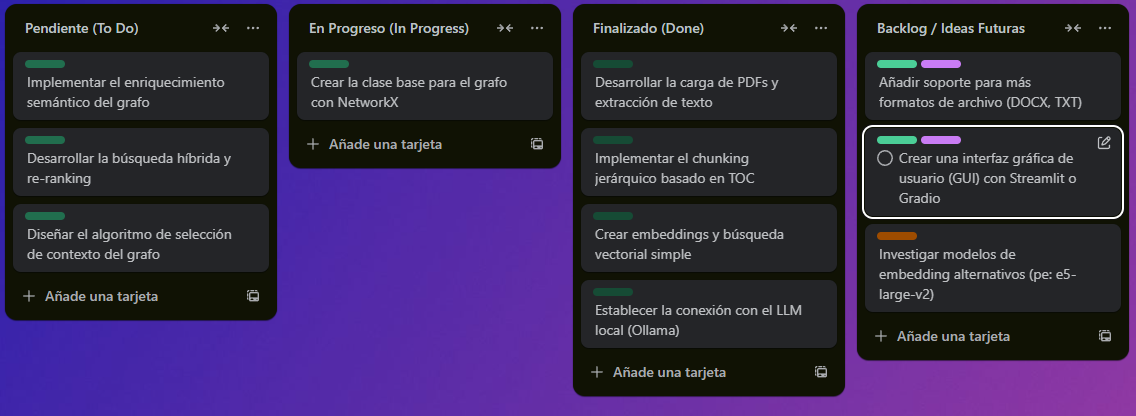
\includegraphics[width=0.9\textwidth]{images/kanban_fin_incremento1.png} % Cambia esto a la ruta de tu imagen
    \caption{Captura del tablero Kanban al finalizar el Incremento 1 (Semana 9).}
    \label{fig:kanban_inc1}
\end{figure}
\newpage
\section*{Estado del Tablero al Finalizar el Incremento 2}
Tras la finalización del segundo incremento, el tablero (Figura \ref{fig:kanban_inc2}) refleja la implementación de las funcionalidades de GraphRAG. Las tareas relacionadas con la creación de grafos y la búsqueda híbrida se encuentran ahora completadas. Las tareas del último incremento, centradas en los agentes, están a punto de comenzar.

\begin{figure}[H]
    \centering
    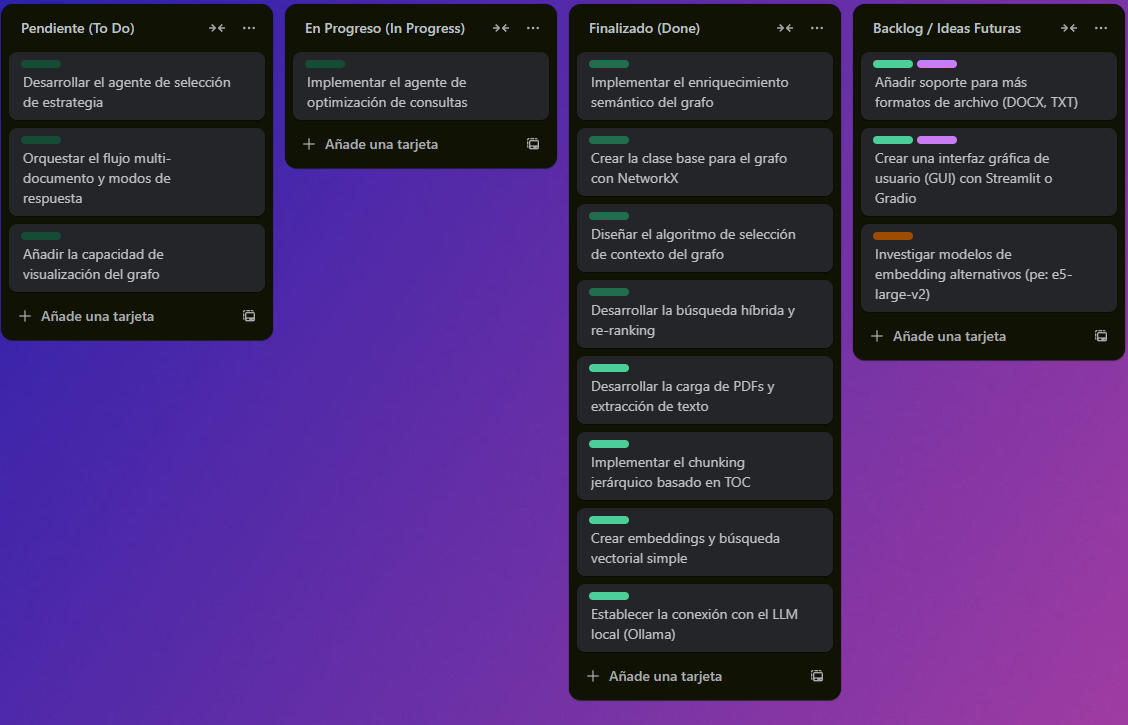
\includegraphics[width=0.9\textwidth]{images/kanban_fin_incremento2.png} % Cambia esto a la ruta de tu imagen
    \caption{Captura del tablero Kanban al finalizar el Incremento 2 (Semana 11).}
    \label{fig:kanban_inc2}
\end{figure}
\newpage
\section*{Estado del Tablero al Finalizar el Incremento 3}
La Figura \ref{fig:kanban_inc3} presenta el estado final del tablero una vez completado todo el desarrollo de software. Todas las tareas de implementación, incluyendo la integración de los agentes inteligentes y la gestión de múltiples documentos, han sido movidas a la columna \textit{Finalizado (Done)}, marcando la conclusión exitosa de la fase de desarrollo.

\begin{figure}[H]
    \centering
    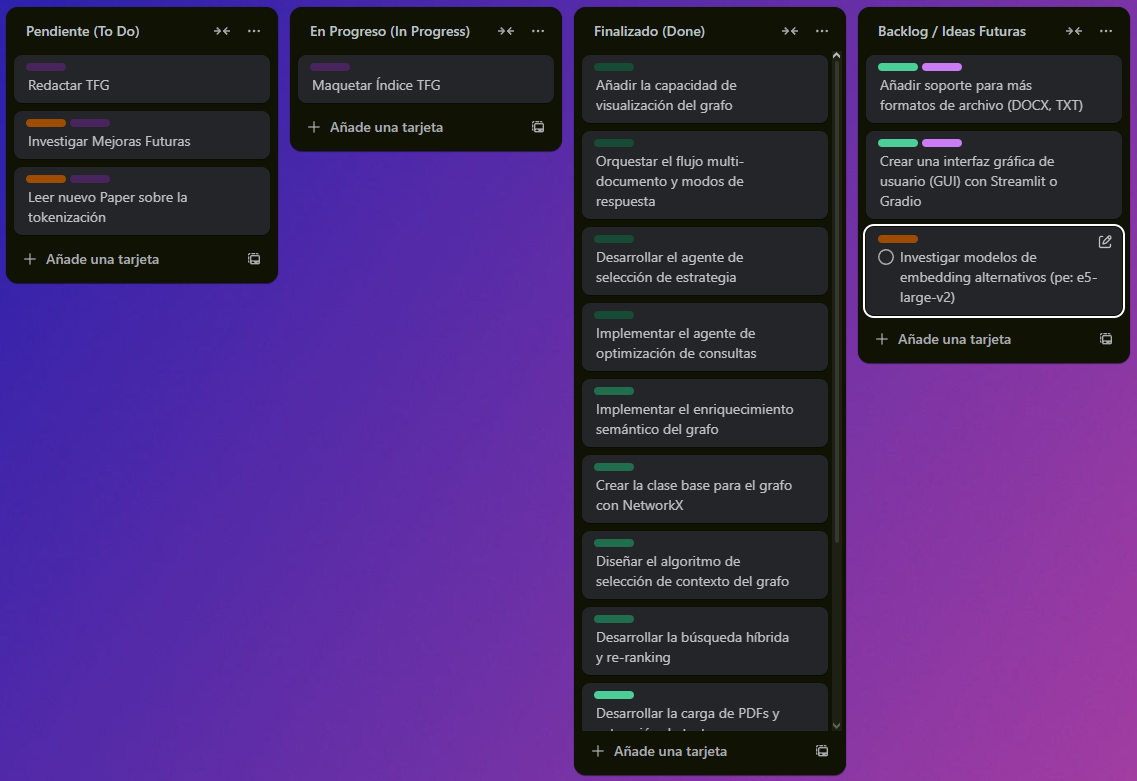
\includegraphics[width=0.9\textwidth]{images/kanban_fin_incremento3.png} % Cambia esto a la ruta de tu imagen
    \caption{Captura del tablero Kanban al finalizar la fase de implementación (Semana 12).}
    \label{fig:kanban_inc3}
\end{figure}
      \chapter{Manual de Usuario e Instalación}
\label{ape:manual}

Este anexo proporciona las instrucciones necesarias para la puesta en marcha y operación del sistema en un entorno local, incluyendo los requisitos de hardware y software, el procedimiento de instalación paso a paso, la guía de operación con ejemplos reales y una sección de resolución de problemas comunes.

\section{Requisitos del Sistema}

\subsection{Hardware recomendado}
Para una ejecución fluida de los modelos locales, se recomienda:
\begin{itemize}
    \item \textbf{GPU:} NVIDIA con arquitectura CUDA (mínimo 8 GB VRAM, ej. RTX 3060/4050 o superior). Sin GPU, el sistema opera por CPU con tiempos de ingesta significativamente mayores.
    \item \textbf{RAM:} 16 GB o superior. El sistema mantiene los grafos de todos los documentos cargados en memoria durante la sesión (aproximadamente 15 MB por cada 100 páginas procesadas).
    \item \textbf{Almacenamiento:} Mínimo 10 GB de espacio libre para alojar los modelos de lenguaje descargados por \texttt{Ollama} y los modelos de \textit{embeddings} de \texttt{sentence-transformers}.
\end{itemize}

\subsection{Software necesario}
\begin{itemize}
    \item \textbf{Python 3.10} o superior.
    \item \textbf{Ollama:} Motor de inferencia local. Disponible en \url{https://ollama.com}. Debe estar en ejecución como servicio en segundo plano antes de iniciar el sistema.
    \item \textbf{NVIDIA CUDA Toolkit:} Versión 12.x para aceleración por hardware. Descargable desde \url{https://developer.nvidia.com/cuda-downloads}.
    \item \textbf{Git:} Para clonar el repositorio del proyecto.
\end{itemize}

\section{Instalación y Configuración}

\subsection{Paso 1: Obtención del código fuente}
Clone el repositorio del proyecto en su directorio de trabajo:
\begin{verbatim}
git clone <URL_del_repositorio>
cd <nombre_del_directorio>
\end{verbatim}
Sustituya \texttt{<URL\_del\_repositorio>} por la URL real del repositorio.

\subsection{Paso 2: Preparación del entorno virtual}
Se recomienda el uso de un entorno virtual de Python para aislar las dependencias del proyecto:
\begin{verbatim}
python -m venv venv

# En Linux/macOS:
source venv/bin/activate

# En Windows:
venv\Scripts\activate
\end{verbatim}
Una vez activado el entorno, instale todas las dependencias del proyecto:
\begin{verbatim}
pip install -r requirements.txt
\end{verbatim}

\subsection{Paso 3: Descarga de modelos en Ollama}
Con \texttt{Ollama} instalado y en ejecución, descargue el modelo de lenguaje principal:
\begin{verbatim}
ollama pull llama3.1:8b
\end{verbatim}
Este proceso requiere una conexión a internet y descarga aproximadamente 4,7 GB. Los modelos de \textit{embeddings} (\texttt{sentence-transformers/all-MiniLM-L6-v2} y el \textit{cross-encoder}) se descargan automáticamente desde HuggingFace en la primera ejecución del sistema.

\subsection{Paso 4: Preparación de los documentos}
Coloque los archivos PDF que desea analizar en el directorio \texttt{Code/MVP/Pliegos/} del proyecto (o modifique la variable de ruta al inicio de \texttt{main.py} para apuntar a su directorio de documentos):
\begin{verbatim}
mkdir Code/MVP/Pliegos
cp /ruta/a/sus/pliegos/*.pdf Code/MVP/Pliegos/
\end{verbatim}

\section{Guía de Operación}

\subsection{Inicio del sistema}
Asegúrese de que \texttt{Ollama} esté en ejecución en segundo plano y, con el entorno virtual activado, ejecute el script principal:
\begin{verbatim}
python main.py
\end{verbatim}
Al iniciarse, el sistema procesará automáticamente todos los PDFs del directorio configurado. Verá en la consola el progreso de extracción, generación de \textit{embeddings} y construcción del grafo para cada documento. Una vez finalizada la fase de ingesta, aparecerá el \textit{prompt} interactivo de chat.

\subsection{Comandos de control}
Durante la sesión de chat, el usuario puede utilizar los siguientes comandos especiales para gestionar el comportamiento del sistema:

\begin{table}[ht]
\centering
\begin{tabularx}{\textwidth}{|l|X|}
\hline
\textbf{Comando} & \textbf{Efecto} \\ \hline
\texttt{modo 1} & Cambia a respuestas individuales por documento. Cada PDF recibe y responde la consulta de forma independiente. Modo por defecto. \\ \hline
\texttt{modo 2} & Activa el modo consolidado multidocumento. El sistema extrae subgrafos de todos los documentos y genera una única respuesta integrada. \\ \hline
\texttt{visualizar si} & Activa la generación de archivos \texttt{.png} con la representación visual del subgrafo de consulta tras cada respuesta. \\ \hline
\texttt{visualizar no} & Desactiva la generación de visualizaciones (comportamiento por defecto). \\ \hline
\texttt{salir} & Finaliza la ejecución del programa de forma limpia. \\ \hline
\end{tabularx}
\caption{Comandos de control disponibles en la interfaz interactiva.}
\label{tab:comandos}
\end{table}

\subsection{Ejemplos de consultas}

A continuación se presentan ejemplos representativos de consultas y el tipo de respuesta que genera el sistema:

\textbf{Consulta específica (modo PARTIAL):}

\medskip\noindent\textit{¿Qué medidas de seguridad física exige el pliego para el rack de comunicaciones?}

El agente de estrategia selecciona \texttt{PARTIAL}, el optimizador reformula la consulta a \textit{``seguridad física rack comunicaciones''}, y el sistema recupera el nodo correspondiente junto con su sección padre. La respuesta detalla los requisitos de anclaje, cierre y acceso restringido del \textit{rack}.

\textbf{Consulta de síntesis global (modo FULL):}

\medskip\noindent\textit{Resume los principales requisitos técnicos del sistema de videovigilancia.}

El agente detecta la necesidad de síntesis y selecciona \texttt{FULL}, enviando al LLM el contenido completo del documento. La respuesta consolida los requisitos de resolución de cámara, almacenamiento y conectividad en una lista estructurada.

\textbf{Consulta multidocumento (modo 2):}

\medskip\noindent\textit{Compara los plazos de entrega del pliego técnico y el administrativo.}

Con el modo 2 activo, el sistema consulta ambos grafos de forma simultánea y genera una respuesta que cita explícitamente cada documento, señalando posibles inconsistencias entre ellos.

\section{Resolución de Problemas Frecuentes}

\begin{description}
    \item[El sistema no detecta secciones del índice correctamente.] Este problema suele darse en documentos cuyo índice no contiene hipervínculos internos o cuya numeración de secciones es irregular. El sistema intentará la extracción mediante expresiones regulares como mecanismo de \textit{fallback}. Si los resultados siguen siendo incorrectos, verifique que el PDF no esté protegido contra la extracción de texto o que no sea un documento escaneado sin capa OCR.

    \item[Ollama no responde o lanza un error de conexión.] Compruebe que el servicio de \texttt{Ollama} esté en ejecución ejecutando \texttt{ollama list} desde la terminal. Si el servicio no aparece, inícielo con \texttt{ollama serve}. Verifique también que el puerto por defecto (11434) no esté bloqueado por el cortafuegos del sistema.

    \item[Error de memoria insuficiente (CUDA out of memory).] El modelo \texttt{llama3.1:8b} cuantizado a 4-bit requiere aproximadamente 5,2 GB de VRAM. Si su GPU dispone de menos memoria, puede intentar usar el modelo en su variante de menor tamaño (\texttt{llama3.2:3b}) ejecutando \texttt{ollama pull llama3.2:3b} y configurando el nombre del modelo en el código fuente.

    \item[Los tiempos de ingesta son muy elevados.] Si el sistema opera en modo CPU (sin GPU NVIDIA o sin CUDA instalado), los tiempos de generación de \textit{embeddings} pueden ser entre $3\times$ y $5\times$ superiores. Asegúrese de que \texttt{CUDA Toolkit 12.x} esté correctamente instalado y de que \texttt{torch} detecte la GPU ejecutando:
\begin{verbatim}
python -c "import torch; print(torch.cuda.is_available())"
\end{verbatim}

    \item[El sistema genera un chunk que mezcla contenido de secciones distintas.] Esto ocurre ocasionalmente cuando los títulos de sección tienen una similitud textual muy alta y el \textit{fuzzy matching} no puede distinguirlos con precisión. En ese caso, puede ajustar el umbral de similitud difusa en el archivo de configuración de \texttt{chunk\_extractor.py}.
\end{description}

      
      % La bibliografía se genera automágicamente
      % Yo prefiero incluírla en el "mainmatter"
      \bibliographystyle{unsrt}
      \bibliography{refs}
   % Material final del documento (glosarios, índice y contraportada)
   % Aquí pueden ir los apéndices aunque pueden subirse.
   \backmatter
\end{document}
